\documentclass[10]{article}
%\documentclass[11pt]{book}
\usepackage{hyperref}
\usepackage{amsfonts,amssymb,amsmath,amsthm,cite}
\usepackage{graphicx}
\usepackage[toc,page]{appendix}
\usepackage{nicefrac}
%% \usepackage[francais]{babel}
\usepackage[applemac]{inputenc}
\usepackage{amssymb, euscript}
\usepackage[matrix,arrow,curve]{xy}
\usepackage{graphicx}
\usepackage{tabularx}
\usepackage{float}
\usepackage{tikz}
\usepackage{slashed}
\usepackage{mathrsfs}
\usepackage{multirow}

%\usepackage{mathtools}

\usetikzlibrary{matrix}

\usepackage{siunitx}

\usepackage{lmodern}
\usepackage[T1]{fontenc}
\usepackage[babel=true]{microtype}


\usepackage{amsfonts,cite}
\usepackage{graphicx}

%% \usepackage[francais]{babel}
\usepackage[applemac]{inputenc}


\usepackage[sc]{mathpazo}
\usepackage{environ}

\linespread{1.05}         % Palatino needs more leading (space between lines)


%\usepackage[usenames]{color}



\DeclareFontFamily{T1}{pzc}{}
\DeclareFontShape{T1}{pzc}{m}{it}{1.8 <-> pzcmi8t}{}
\DeclareMathAlphabet{\mathpzc}{T1}{pzc}{m}{it}
% the command for it is \mathpzc

\textwidth=140mm


% % % % % % % % % % % % % % % % % % % %
\theoremstyle{plain}
\newtheorem{prop}{Proposition}[section]
\newtheorem{prdf}[prop]{Proposition and Definition}
\newtheorem{lem}[prop]{Lemma}%[section]
\newtheorem{cor}[prop]{Corollary}%[section]
\newtheorem{thm}[prop]{Theorem}%[section]
\newtheorem{theorem}[prop]{Theorem}
\newtheorem{lemma}[prop]{Lemma}
\newtheorem{proposition}[prop]{Proposition}
\newtheorem{corollary}[prop]{Corollary}
\newtheorem{statement}[prop]{Statement}

\theoremstyle{definition}
\newtheorem{defn}[prop]{Definition}%[section]
\newtheorem{cordefn}[prop]{Corollary and Definition}%[section]
\newtheorem{empt}[prop]{}%[section]
\newtheorem{exm}[prop]{Example}%[section]
\newtheorem{rem}[prop]{Remark}%[section]
\newtheorem{prob}[prop]{Problem}
\newtheorem{conj}{Conjecture}       %% Hypothesis 1
\newtheorem{cond}{Condition}        %% Condition 1
%\newtheorem{axiom}[thm]{Axiom}           %% Axiom 1 modified
\newtheorem{fact}[prop]{Fact}
\newtheorem{ques}{Question}         %% Question 1
\newtheorem{answ}{Answer}           %% Answer 1
\newtheorem{notn}{Notation}        %% Notations are not numbered

\theoremstyle{definition}
\newtheorem{notation}[prop]{Notation}
\newtheorem{definition}[prop]{Definition}
\newtheorem{example}[prop]{Example}
\newtheorem{exercise}[prop]{Exercise}
\newtheorem{conclusion}[prop]{Conclusion}
\newtheorem{conjecture}[prop]{Conjecture}
\newtheorem{criterion}[prop]{Criterion}
\newtheorem{summary}[prop]{Summary}
\newtheorem{axiom}[prop]{Axiom}
\newtheorem{problem}[prop]{Problem}
%\theoremstyle{remark}
\newtheorem{remark}[prop]{Remark}

\numberwithin{equation}{section}
\newtheorem*{claim}{Claim}
\DeclareMathOperator{\Dom}{Dom}              %% domain of an operator
\newcommand{\Dslash}{{D\mkern-11.5mu/\,}}    %% Dirac operator


%\newcommand\myeq{\stackrel{\mathclap{\normalfont\mbox{def}}}{=}}
\newcommand{\nor}[1]{\left\Vert #1\right\Vert}    %\nor{x}=||x||
\newcommand{\vertiii}[1]{{\left\vert\kern-0.25ex\left\vert\kern-0.25ex\left\vert #1
		\right\vert\kern-0.25ex\right\vert\kern-0.25ex\right\vert}}
\newcommand{\Ga}{\Gamma}  
\newcommand{\coker}{\mathrm{coker}}                   %% short for  \Gamma
\newcommand{\Coo}{C^\infty}                  %% smooth functions
% % % % % % % % % % % % % % % % % % % %


\usepackage[sc]{mathpazo}
\linespread{1.05}         % Palatino needs more leading (space between lines)

\newbox\ncintdbox \newbox\ncinttbox %% noncommutative integral symbols
\setbox0=\hbox{$-$} \setbox2=\hbox{$\displaystyle\int$}
\setbox\ncintdbox=\hbox{\rlap{\hbox
		to \wd2{\hskip-.125em \box2\relax\hfil}}\box0\kern.1em}
\setbox0=\hbox{$\vcenter{\hrule width 4pt}$}
\setbox2=\hbox{$\textstyle\int$} \setbox\ncinttbox=\hbox{\rlap{\hbox
		to \wd2{\hskip-.175em \box2\relax\hfil}}\box0\kern.1em}

\newcommand{\ncint}{\mathop{\mathchoice{\copy\ncintdbox}%
		{\copy\ncinttbox}{\copy\ncinttbox}%
		{\copy\ncinttbox}}\nolimits}  %% NC integral

%%% Repeated relations:
\newcommand{\xyx}{\times\cdots\times}      %% repeated product
\newcommand{\opyop}{\oplus\cdots\oplus}    %% repeated direct sum
\newcommand{\oxyox}{\otimes\cdots\otimes}  %% repeated tensor product
\newcommand{\wyw}{\wedge\cdots\wedge}      %% repeated exterior product
\newcommand{\subysub}{\subset\hdots\subset}      %% repeated subset
\newcommand{\supysup}{\supset\hdots\supset}      %% repeated supset
\newcommand{\rep}{\mathfrak{rep}}
\newcommand{\lift}{\mathfrak{lift}}
\newcommand{\desc}{\mathfrak{desc}}
%%% Roman letters:
\newcommand{\id}{\mathrm{id}}                %% identity map
\newcommand{\Id}{\mathrm{Id}}                %% identity map
\newcommand{\pt}{\mathrm{pt}}                %% a point
\newcommand{\const}{\mathrm{const}}          %% a constant
\newcommand{\codim}{\mathrm{codim}}          %% codimension
\newcommand{\cyc}{\mathrm{cyclic}}  %% cyclic sum
\renewcommand{\d}{\mathrm{d}}       %% commutative differential
\newcommand{\dR}{\mathrm{dR}}       %% de~Rham cohomology
\newcommand{\proj}{\mathrm{proj}}                %% a projection
\newcommand*{\braket}[2]{\langle#1 {,~} #2\rangle}% right inner products
\newcommand*{\lbraket}[2]{\langle\!\langle#1{\mid}#2\rangle\!\rangle}% left inner products

\newcommand*{\Mult}{\mathcal M}% multiplier algebra
\newcommand{\Lt}{\mathcal{L}}                 %%\newcommand{\unitsv}[1]{#1^{(0)}}

\newcommand{\A}{\mathcal{A}}                 %%\newcommand{\unitsv}[1]{#1^{(0)}}
\newcommand{\units}{G^{(0)}}
\newcommand{\haars}{\{\lambda^{u}\}_{u\in\units}}
\newcommand{\shaars}{\{\lambda_{u}\}_{u\in\units}}
\newcommand{\haarsv}[2]{\{\lambda^{#2}_{#1}\}_{#2\in\unitsv{#1}}}
\newcommand{\haarv}[2]{\lambda^{#2}_{#1}}

\renewcommand{\a}{\alpha}                    %% short for  \alphapha
\DeclareMathOperator{\ad}{ad}                %% infml adjoint repn
\newcommand{\as}{\quad\mbox{as}\enspace}     %% `as' with spacing
\newcommand{\Aun}{\widetilde{\mathcal{A}}}   %% unital algebra
\newcommand{\B}{\mathcal{B}}                 %% space of distributions
\newcommand{\E}{\mathcal{E}}                 %% space of distributions
\renewcommand{\b}{\beta}                     %% short for \beta
\newcommand{\braCket}[3]{\langle#1\mathbin|#2\mathbin|#3\rangle}
%\newcommand{\braket}[2]{\langle#1\mathbin|#2\rangle} %% <w|z>
\newcommand{\C}{\mathbb{C}}                  %% complex numbers
\newcommand{\CC}{\mathcal{C}}                %% space of distributions
\newcommand{\cc}{\mathbf{c}}                 %% Hochschild cycle
\DeclareMathOperator{\Cl}{C\ell}             %% Clifford algebra
\newcommand{\F}{\mathcal{F}}                 %% space of test functions
\newcommand{\G}{\mathcal{G}}                 %% 
\newcommand{\D}{\mathcal{D}}                 %% Moyal L^2-filtration
\renewcommand{\H}{\mathcal{H}}               %% Hilbert space
\newcommand{\half}{\tfrac{1}{2}}             %% small fraction  1/2
\newcommand{\hh}{\mathcal{H}}                %% Hilbert space
\newcommand{\hookto}{\hookrightarrow}        %% abbreviation
\newcommand{\Ht}{{\widetilde{\mathcal{H}}}}  %% Hilbert space of forms
\newcommand{\I}{\mathcal{I}}                 %% tracelike functions
\DeclareMathOperator{\Junk}{Junk}            %% the junk DGA ideal
\newcommand{\K}{\mathcal{K}}                 %% compact operators
\newcommand{\ket}[1]{|#1\rangle}             %% ket vector
\newcommand{\ketbra}[2]{|#1\rangle\langle#2|} %% rank one operator
\renewcommand{\L}{\mathcal{L}}               %% operator algebra
\newcommand{\La}{\Lambda}                    %% short for \Lambda
\newcommand{\la}{\lambda}                    %% short for \lambda
\newcommand{\lf}{L_f^\theta}                 %% left mult operator
\newcommand{\M}{\mathcal{M}}                 %% Moyal multplr algebra
\newcommand{\Lb}{\mathcal{L}}                 %% Moyal multplr algebra
\newcommand{\mm}{\mathcal{M}^\theta}
%\newcommand{{{\star_{\theta}}}{{\mathchoice{\mathbin{\;|\;ar_{_\theta}}}
			%            {\mathbin{\;|\;ar_{_\theta}}}           %% Moyal
			%            {{\;|\;ar_\theta}}{{\;|\;ar_\theta}}}}    %% product
	\newcommand{\N}{\mathbb{N}}                  %% nonnegative integers
	\newcommand{\NN}{\mathcal{N}}                %% a Moyal algebra
	\newcommand{\nb}{\nabla}                     %% gradient
	\newcommand{\Oh}{\mathcal{O}}                %% comm multiplier alg
	\newcommand{\om}{\omega}                     %% short for \omega
	\newcommand{\opp}{{\mathrm{op}}}             %% opposite algebra
	\newcommand{\ox}{\otimes}                    %% tensor product
	\newcommand{\eps}{\varepsilon}                    %% tensor product
	\newcommand{\otimesyox}{\otimes\cdots\otimes}    %% repeated tensor product
	\newcommand{\pa}{\partial}                   %% short for \partial
	\newcommand{\pd}[2]{\frac{\partial#1}{\partial#2}}%% partial derivative
	\newcommand{\piso}[1]{\lfloor#1\rfloor}      %% integer part
	\newcommand{\PsiDO}{\Psi~\mathrm{DO}}         %% pseudodiffl operators
	\newcommand{\Q}{\mathbb{Q}}                  %% rational numbers
	\newcommand{\R}{\mathbb{R}}                  %% real numbers
	\newcommand{\rdl}{R_\Dslash(\lambda)}        %% resolvent
	\newcommand{\roundbraket}[2]{(#1\mathbin|#2)} %% (w|z)
	\newcommand{\row}[3]{{#1}_{#2},\dots,{#1}_{#3}} %% list: a_1,...,a_n
	\newcommand{\sepword}[1]{\quad\mbox{#1}\quad} %% well-spaced words
	\newcommand{\set}[1]{\{\,#1\,\}}             %% set notation
	\newcommand{\Sf}{\mathbb{S}}                 %% sphere
	\newcommand{\uhor}[1]{\Omega^1_{hor}#1}
	\newcommand{\sco}[1]{{\sp{(#1)}}}
	\newcommand{\sw}[1]{{\sb{(#1)}}}
	\DeclareMathOperator{\spec}{sp}              %% spectrum
	\renewcommand{\SS}{\mathcal{S}}              %% Schwartz space
	\newcommand{\sss}{\mathcal{S}}               %% Schwartz space
	\DeclareMathOperator{\supp}{\mathfrak{supp}}            %% support
	\newcommand{\T}{\mathbb{T}}                  %% circle as a group
	\renewcommand{\th}{\theta}                   %% short for \theta
	\newcommand{\thalf}{\tfrac{1}{2}}            %% small* fraction 1/2
	\newcommand{\tihalf}{\tfrac{i}{2}}           %% small* fraction i/2
	\newcommand{\tpi}{{\tilde\pi}}               %% extended representation
	\DeclareMathOperator{\Tr}{Tr}                %% trace of operator
	\DeclareMathOperator{\tr}{tr}                %% trace of matrix
	\newcommand{\del}{\partial}                  %% short for  \partial
	\DeclareMathOperator{\tsum}{{\textstyle\sum}} %% small sum in display
	\newcommand{\V}{\mathcal{V}}                 %% test function space
	\newcommand{\vac}{\ket{0}}                   %% vacuum ket vector
	\newcommand{\vf}{\varphi}                    %% scalar field
	\newcommand{\w}{\wedge}                      %% exterior product
	\DeclareMathOperator{\wres}{wres}            %% density of Wresidue
	\newcommand{\x}{\times}                      %% cross
	\newcommand{\Z}{\mathbb{Z}}                  %% integers
	\newcommand{\7}{\dagger}                     %% short for + symbol
	\newcommand{\8}{\bullet}                     %% anonymous degree
	\renewcommand{\.}{\cdot}                     %% anonymous variable
	\renewcommand{\:}{\colon}                    %% colon in  f: A -> B
	
	%\newcommand{\sA}{\mathscr{A}}       %%
	\newcommand{\sA}{\mathcal{A}} 
	\newcommand{\sB}{\mathcal{B}}       %%
	\newcommand{\sC}{\mathcal{C}}       %%
	\newcommand{\sD}{\mathcal{D}}       %%
	\newcommand{\sE}{\mathcal{E}}       %%
	\newcommand{\sF}{\mathcal{F}}       %%
	\newcommand{\sG}{\mathcal{G}}       %%
	\newcommand{\sH}{\mathcal{H}}       %%
	\newcommand{\sI}{\mathcal{I}}       %%
	\newcommand{\sJ}{\mathcal{J}}       %%
	\newcommand{\sK}{\mathcal{K}}       %%
	\newcommand{\sL}{\mathcal{L}}       %%
	\newcommand{\sM}{\mathcal{M}}       %%
	\newcommand{\sN}{\mathcal{N}}       %%
	\newcommand{\sO}{\mathcal{O}}       %%
	\newcommand{\sP}{\mathcal{P}}       %%
	\newcommand{\sQ}{\mathcal{Q}}       %%
	\newcommand{\sR}{\mathcal{R}}       %%
	\newcommand{\sS}{\mathcal{S}}       %%
	\newcommand{\sT}{\mathcal{T}}       %%
	\newcommand{\sU}{\mathcal{U}}       %%
	\newcommand{\sV}{\mathcal{V}}       %%
	\newcommand{\sX}{\mathcal{X}}       %%
	\newcommand{\sY}{\mathcal{Y}}       %%
	\newcommand{\sZ}{\mathcal{Z}}       %%
	
	\newcommand{\Om}{\Omega}       %%
	
	
	\DeclareMathOperator{\ptr}{ptr}     %% Poisson trace
	\DeclareMathOperator{\Trw}{Tr_\omega} %% Dixmier trace
	\DeclareMathOperator{\vol}{Vol}     %% total volume
	\DeclareMathOperator{\Vol}{Vol}     %% total volume
	\DeclareMathOperator{\Area}{Area}   %% area of a surface
	\DeclareMathOperator{\Wres}{Wres}   %% (Wodzicki) residue
	
	\newcommand{\dd}[1]{\frac{\partial}{\partial#1}}   %% partial derivation
	\newcommand{\ddt}[1]{\frac{d}{d#1}}                %% derivative
	\newcommand{\inv}[1]{\frac{1}{#1}}                 %% inverse
	\newcommand{\sfrac}[2]{{\scriptstyle\frac{#1}{#2}}} %% tiny fraction
	
	\newcommand{\bA}{\mathbb{A}}       %%
	\newcommand{\bB}{\mathbb{B}}       %%
	\newcommand{\bC}{\mathbb{C}}       %%
	\newcommand{\bCP}{\mathbb{C}P}     %%
	\newcommand{\bD}{\mathbb{D}}       %%
	\newcommand{\bE}{\mathbb{E}}       %%
	\newcommand{\bF}{\mathbb{F}}       %%
	\newcommand{\bG}{\mathbb{G}}       %%
	\newcommand{\bH}{\mathbb{H}}       %%
	\newcommand{\bHP}{\mathbb{H}P}     %%
	\newcommand{\bI}{\mathbb{I}}       %%
	\newcommand{\bJ}{\mathbb{J}}       %%
	\newcommand{\bK}{\mathbb{K}}       %%
	\newcommand{\bL}{\mathbb{L}}       %%
	\newcommand{\bM}{\mathbb{M}}       %%
	\newcommand{\bN}{\mathbb{N}}       %%
	\newcommand{\bO}{\mathbb{O}}       %%
	\newcommand{\bOP}{\mathbb{O}P}     %%
	\newcommand{\bP}{\mathbb{P}}       %%
	\newcommand{\bQ}{\mathbb{Q}}       %%
	\newcommand{\bR}{\mathbb{R}}       %%
	\newcommand{\bRP}{\mathbb{R}P}     %%
	\newcommand{\bS}{\mathbb{S}}       %%
	\newcommand{\bT}{\mathbb{T}}       %%
	\newcommand{\bU}{\mathbb{U}}       %%
	\newcommand{\bV}{\mathbb{V}}       %%
	\newcommand{\bX}{\mathbb{X}}       %%
	\newcommand{\bY}{\mathbb{Y}}       %%
	\newcommand{\bZ}{\mathbb{Z}}       %%
	
	\newcommand{\bydef}{\stackrel{\mathrm{def}}{=}}          %% 
	\newcommand{\defeq}{\stackrel{\mathrm{def}}{=}}   
	
	
	
	\newcommand{\al}{\alpha}          %% short for  \alpha
	\newcommand{\bt}{\beta}           %% short for  \beta
	\newcommand{\Dl}{\Delta}          %% short for  \Delta
	\newcommand{\dl}{\delta}          %% short for  \delta
	\newcommand{\ga}{\gamma}          %% short for  \gamma
	\newcommand{\ka}{\kappa}          %% short for  \kappa
	\newcommand{\sg}{\sigma}          %% short for  \sigma
	\newcommand{\Sg}{\Sigma}          %% short for  \Sigma
	\newcommand{\Th}{\Theta}          %% short for  \Theta
	\renewcommand{\th}{\theta}        %% short for  \theta
	\newcommand{\vth}{\vartheta}      %% short for  \vartheta
	\newcommand{\ze}{\zeta}           %% short for  \zeta
	
	\DeclareMathOperator{\ord}{ord}     %% order of a PsiDO
	\DeclareMathOperator{\rank}{rank}   %% rank of a vector bundle
	\DeclareMathOperator{\sign}{sign}   %%
	\DeclareMathOperator{\sgn}{sgn}   %%
	\DeclareMathOperator{\chr}{char}   %%
	\DeclareMathOperator{\ev}{ev}       %% evaluation
	
	
	\newcommand{\Op}{\mathbf{Op}}
	\newcommand{\As}{\mathbf{As}}
	\newcommand{\Com}{\mathbf{Com}}
	\newcommand{\LLie}{\mathbf{Lie}}
	\newcommand{\Leib}{\mathbf{Leib}}
	\newcommand{\Zinb}{\mathbf{Zinb}}
	\newcommand{\Poiss}{\mathbf{Poiss}}
	
	\newcommand{\gX}{\mathfrak{X}}      %% vector fields
	\newcommand{\sol}{\mathfrak{so}}    %% special orthogonal Lie algebra
	\newcommand{\gm}{\mathfrak{m}}      %% maximal ideal
	
	
	\DeclareMathOperator{\Res}{Res}
	\DeclareMathOperator{\NCRes}{NCRes}
	\DeclareMathOperator{\Ind}{Ind}
	%% co/homology theories
	\DeclareMathOperator{\rH}{H}        %% any co/homology
	\DeclareMathOperator{\rC}{C}        %%  any co/chains
	\DeclareMathOperator{\rZ}{Z}        %% cycles
	\DeclareMathOperator{\rB}{B}        %% boundaries
	\DeclareMathOperator{\rF}{F}        %% filtration
	\DeclareMathOperator{\Gr}{gr}        %% associated graded object
	\DeclareMathOperator{\rHc}{H_{\mathrm{c}}}   %% co/homology with compact support
	\DeclareMathOperator{\drH}{H_{\mathrm{dR}}}  %% de Rham co/homology
	\DeclareMathOperator{\cechH}{\check{H}}    %% Cech co/homology
	\DeclareMathOperator{\rK}{K}        %% K-groups
	\DeclareMathOperator{\rKO}{KO}        %% real K-groups
	\DeclareMathOperator{\rKU}{KU}        %% unitary K-groups
	\DeclareMathOperator{\rKSp}{KSp}        %% symplectic K-groups
	\DeclareMathOperator{\rR}{R}        %% representation ring
	\DeclareMathOperator{\rI}{I}        %% augmentation ideal
	\DeclareMathOperator{\HH}{HH}       %% Hochschild co/homology
	\DeclareMathOperator{\HC}{HC}       %% cyclic co/homology
	\DeclareMathOperator{\HP}{HP}       %% periodic cyclic co/homology
	\DeclareMathOperator{\HN}{HN}       %% negative cyclic co/homology
	\DeclareMathOperator{\HL}{HL}       %% Leibniz co/homology
	\DeclareMathOperator{\KK}{KK}       %% KK-theory
	\DeclareMathOperator{\KKK}{\mathbf{KK}}       %% KK-theory as a category
	\DeclareMathOperator{\Ell}{Ell}       %% Abstract elliptic operators
	\DeclareMathOperator{\cd}{cd}       %% cohomological dimension
	\DeclareMathOperator{\spn}{span}       %% span
	\DeclareMathOperator{\linspan}{span} %% linear span (can't use \span)
	\newcommand{\blank}{-}   
	
	
	
	\newcommand{\twobytwo}[4]{\begin{pmatrix} #1 & #2 \\ #3 & #4 \end{pmatrix}}
	\newcommand{\CGq}[6]{C_q\!\begin{pmatrix}#1&#2&#3\\#4&#5&#6\end{pmatrix}}
	%% q-Clebsch--Gordan coefficients
	\newcommand{\cz}{{\bullet}}         %% anonymous degree
	\newcommand{\nic}{{\vphantom{\dagger}}} %% invisible dagger
	\newcommand{\ep}{{\dagger}}         %% abbreviation for + symbol
	\newcommand{\downto}{\downarrow}    %% right hand limit
	\newcommand{\isom}{\cong}          %% isomorphism
	\newcommand{\lt}{\triangleright}    %% a left action
	\newcommand{\otto}{\leftrightarrow} %% bijection
	\newcommand{\rt}{\triangleleft}     %% a right action
	\newcommand{\semi}{\rtimes}         %% crossed product
	\newcommand{\tensor}{\otimes}       %% tensor product
	\newcommand{\cotensor}{\square}       %% cotensor product
	\newcommand{\trans}{\pitchfork}     %% transverse
	\newcommand{\ul}{\underline}        %% for sheaves
	\newcommand{\upto}{\uparrow}        %% left hand limit
	\renewcommand{\:}{\colon}           %% colon in  f: A -> B
	\newcommand{\blt}{\ast}
	\newcommand{\Co}{C_{\bullet}}
	\newcommand{\cCo}{C^{\bullet}}
	\newcommand{\nbs}{\nabla^S}         %% spin connection
	\newcommand{\up}{{\mathord{\uparrow}}} %% `up' spinors
	\newcommand{\dn}{{\mathord{\downarrow}}} %% `down' spinors
	\newcommand{\updn}{{\mathord{\updownarrow}}} %% up or down
	
	%%% Bilinear enclosures:
	
	\newcommand{\bbraket}[2]{\langle\!\langle#1\stroke#2\rangle\!\rangle}
	%% <<w|z>>
	\newcommand{\bracket}[2]{\langle#1,\, #2\rangle} %% <w,z>
	\newcommand{\scalar}[2]{\langle#1,\,#2\rangle} %% <w,z>
	\newcommand{\poiss}[2]{\{#1,\,#2\}} %% {w,z}
	\newcommand{\dst}[2]{\langle#1,#2\rangle} %% distributions <u,\phi>
	\newcommand{\pairing}[2]{(#1\stroke #2)} %% right-linear pairing
	\def\<#1|#2>{\langle#1\stroke#2\rangle} %% \braket (Dirac notation)
	\def\?#1|#2?{\{#1\stroke#2\}}        %% left-linear pairing
	
	%%% Accent-like macros:
	
	\renewcommand{\Bar}[1]{\overline{#1}} %% closure operator
	\renewcommand{\Hat}[1]{\widehat{#1}}  %% short for \widehat
	\renewcommand{\Tilde}[1]{\widetilde{#1}} %% short for \widetilde
	
	
	\DeclareMathOperator{\bCl}{\bC l}   %% complex Clifford algebra
	
	%%% Small fractions in displays:
	
	\newcommand{\ihalf}{\tfrac{i}{2}}   %% small fraction  i/2
	\newcommand{\quarter}{\tfrac{1}{4}} %% small fraction  1/4
	\newcommand{\shalf}{{\scriptstyle\frac{1}{2}}}  %% tiny fraction  1/2
	\newcommand{\third}{\tfrac{1}{3}}   %% small fraction  1/3
	\newcommand{\ssesq}{{\scriptstyle\frac{3}{2}}} %% tiny fraction  3/2
	\newcommand{\sesq}{{\mathchoice{\tsesq}{\tsesq}{\ssesq}{\ssesq}}} %% 3/2
	\newcommand{\tsesq}{\tfrac{3}{2}}   %% small fraction  3/2
	
	
	%\newcommand\eqdef{\overset{\mathclap{\normalfont\mbox{def}}}{=}}
	\newcommand\eqdef{\overset{\mathrm{def}}{=}}
	
	
	%+++++++++++++++++++++++++++++++++++
	
	\newcommand{\word}[1]{\quad\text{#1}\enspace} %% well-spaced words
	\newcommand{\words}[1]{\quad\text{#1}\quad} %% better-spaced words
	\newcommand{\su}[1]{{\sp{[#1]}}}
	
	\def\<#1,#2>{\langle#1,#2\rangle}            %% bilinear pairing
	\def\ee_#1{e_{{\scriptscriptstyle#1}}}       %% basis projector
	\def\wick:#1:{\mathopen:#1\mathclose:}       %% Wick-ordered operator
	
	\newcommand{\opname}[1]{\mathop{\mathrm{#1}}\nolimits}
	
	\newcommand{\hideqed}{\renewcommand{\qed}{}} %% to suppress `\qed'
	
	
	%%%%%%%%%%%%%%%%%%%%%%%%%%%%%
	%% 2. Some internal machinery
	%%%%%%%%%%%%%%%%%%%%%%%%%%%%%
	
	\newbox\ncintdbox \newbox\ncinttbox %% noncommutative integral symbols
	\setbox0=\hbox{$-$}
	\setbox2=\hbox{$\displaystyle\int$}
	\setbox\ncintdbox=\hbox{\rlap{\hbox
			to \wd2{\box2\relax\hfil}}\box0\kern.1em}
	\setbox0=\hbox{$\vcenter{\hrule width 4pt}$}
	\setbox2=\hbox{$\textstyle\int$}
	\setbox\ncinttbox=\hbox{\rlap{\hbox
			to \wd2{\hskip-.05em\box2\relax\hfil}}\box0\kern.1em}
	
	\newcommand{\disp}{\displaystyle} %% short for  \displaystyle
	
	%\newcommand{\hideqed}{\renewcommand{\qed}{}} %% no `\qed' at end-proof
	
	\newcommand{\stroke}{\mathbin|}   %% (for `\bbraket' and such)
	\newcommand{\tribar}{|\mkern-2mu|\mkern-2mu|} %% norm bars: |||
	
	%%% Enclose one argument with delimiters:
	
	\newcommand{\bra}[1]{\langle{#1}\rvert} %% bra vector <w|
	\newcommand{\kett}[1]{\lvert#1\rangle\!\rangle} %% ket 2-vector |y>>
	\newcommand{\snorm}[1]{\mathopen{\tribar}{#1}%
		\mathclose{\tribar}}                 %% norm |||x|||
	
	
	\newcommand{\End}{\mathrm{End}}       %%
	\newcommand{\Ext}{\mathrm{Ext}}       %%
	\newcommand{\Hom}{\mathrm{Hom}}       %%
	\newcommand{\Mrt}{\mathrm{Mrt}}       %%
	\newcommand{\grad}{\mathrm{grad}}       %%
	\newcommand{\Spin}{\mathrm{Spin}}       %%
	\newcommand{\Ad}{\mathrm{Ad}}       %%
	\newcommand{\Pic}{\mathrm{Pic}}       %%
	\newcommand{\Aut}{\mathrm{Aut}}       %%
	\newcommand{\Inn}{\mathrm{Inn}}       %%
	\newcommand{\Out}{\mathrm{Out}}       %%
	\newcommand{\Homeo}{\mathrm{Homeo}}       %%
	\newcommand{\Diff}{\mathrm{Diff}}       %%
	\newcommand{\im}{\mathrm{im}}       %%
	
	
	\newcommand{\SO}{\mathrm{SO}}       %%
	\newcommand{\SU}{SU}       %%
	\newcommand{\gso}{\mathfrak{so}}    %% special orthogonal Lie algebra
	\newcommand{\gero}{\mathfrak{o}}    %% orthogonal Lie algebra
	\newcommand{\gspin}{\mathfrak{spin}} %% spin Lie algebra
	\newcommand{\gu}{\mathfrak{u}}      %% unitary Lie algebra
	\newcommand{\gsu}{\mathfrak{su}}    %% special unitary Lie algebra
	\newcommand{\gsl}{\mathfrak{sl}}    %% special linear Lie algebra
	\newcommand{\gsp}{\mathfrak{sp}}    %% symplectic linear Lie algebra
	
	%\newcommand{\bes}{\begin{equation}\begin{split}}
			%\newcommand{\ees}{\end{split}\end{equation}}
	%\NewEnviron{split.enviro}{%
		%	\begin{equation}\begin{split}
				%	\BODY
				%	\end{split}\end{equation}
		%$}
	\newenvironment{splitequation}{\begin{equation}\begin{split}}{\end{split}\end{equation}}
	
	%Begin equation split: Begin equation split = bes
	\newcommand{\bs}{\begin{split}}
		\newcommand{\es}{\end{split}}
	\newcommand{\be}{\begin{equation}}
		\renewcommand{\ee}{\end{equation}}
	\newcommand{\bea}{\begin{eqnarray}}
		\newcommand{\eea}{\end{eqnarray}}
	\newcommand{\bean}{\begin{eqnarray*}}
		\newcommand{\eean}{\end{eqnarray*}}
	\newcommand{\brray}{\begin{array}}
		\newcommand{\erray}{\end{array}}
	\newenvironment{equations}
	{\begin{equation}
			\begin{split}}
			{\end{split}
	\end{equation}}
	\newcommand{\Hsquare}{%
		\text{\fboxsep=-.2pt\fbox{\rule{0pt}{1ex}\rule{1ex}{0pt}}}%
	}
	
	\title{Dixmier�Douady theory for $C^*$-algebras of foliations}
	
	\author
	{\textbf{Petr R. Ivankov*}\\
		e-mail: * monster.ivankov@gmail.com \\
	}
	
	\begin{document}

\maketitle  %\setlength{\parindent}{0pt}
\pagestyle{plain}


%\vspace{1 in}


%\noindent

\begin{abstract}
Dixmier�Douady theory states some properties  of $C^*$-algebras having continuous trace. These algebras uniquely depend on the Dixmier�Douady invariant which is a cohomological cocycle. There are a natural pairings of both continuous trace $C^*$-algebras and their $K$-groups. We prove that there are similar ingredients for $C^*$-algebras of foliations, that is these algebras depend on cohomological cycle, also there are natural pairings of these  $C^*$-algebras and their cohomology groups.
\end{abstract}

\tableofcontents
%\end{abstract}

\section{Grothendieck topology of  $C^*$-of foliations}
\paragraph{}
\begin{lemma}\label{foli_grothendieck_lem}
	The given by the Definition \eqref{foli_haus_defn} Hausdorff blowing-up   \textit{complies with Grothendieck topology} (cf. Definition \ref{blowing_compl_defn}).
\end{lemma} 
\begin{proof}
	One should prove that
	$$
	B = C^*_r\left( M, \F \right)_{\mathrm{Sp\acute{e}}\left(\mathscr P^{\text{comm}}\right)_B}.	
	$$
	for any hereditary subalgebra $B\subset C^*_r\left( M, \F \right)$	
	A $C^*$-algebra $C^*_r\left( M, \F \right)_{\mathrm{Sp\acute{e}}\left(\mathscr P^{\text{comm}}\right)_B}$ is a hereditary subalgebra of $C^*_r\left( M, \F \right)$ generated by subalgebras of $B$, so one has $A_{\mathrm{Sp\acute{e}}\left(\mathscr P^{\text{comm}}\right)_B}\subset B$. If $\pi_a: B \hookto  B\left( \H_a\right) $ is an atomic representation then from the Corollary \ref{hered_representation_cor} it follows that there is a projector $p \in B\left( \H_a\right)$ such that
	$$
	C^*_r\left( M, \F \right)_{\mathrm{Sp\acute{e}}\left(\mathscr P^{\text{comm}}\right)_B} = \left\{a \in C^*_r\left( M, \F \right)| p \pi_a\left( a\right)p = \pi_a\left(a \right) \right\}.
	$$
	If $B \neq C^*_r\left( M, \F \right)_{\mathrm{Sp\acute{e}}\left(\mathscr P^{\text{comm}}\right)_B}$ then  $C^*_r\left( M, \F \right)_{\mathrm{Sp\acute{e}}\left(\mathscr P^{\text{comm}}\right)_B}\subsetneqq B$ (cf. \eqref{blowing_grothendieck_inc_eqn}), therefore
	$p < 1_{B\left( \H_a\right) }$.  If $\sX$ is a spectrum of $B$ then there is $x\in \sX$ and which satisfies to following conditions:
	\begin{itemize}
		\item if $\rep_x: B \to B\left(\H_x\right)$ is a representation which corresponds to $x$ then
		$$
		\rep_x\left(C^*_r\left( M, \F \right)_{\mathrm{Sp\acute{e}}\left(\mathscr P^{\text{comm}}\right)_B} \right) = \left\{\rep_x \left(a\right)\in \rep_x\left( B\right) | \rep_x \left(a\right)= p_x\rep_x \left(a\right)p_x\right\}
		$$
		where $p_x \in B\left(\H_x \right)$ is projector;
		\item 	$p_x < 1_{B\left(\H_x \right) }$.
	\end{itemize}
	From the above condition it follows that there is a rank-one projector $\a \in 	\rep_x\left( B\right)$ such that $\a \perp   \rep_x\left(C^*_r\left( M, \F \right)_{\mathrm{Sp\acute{e}}\left(\mathscr P^{\text{comm}}\right)_B}\right)\H_x$.  There is an element $a \in B$ such that $\rep_x\left(a\right)= \a$. If $\mathfrak{A}$ be a regular cover by foliated charts then from the Corollary \ref{foli_cov_alg_cor} it follows that there is a noncommutative polynomial 
	\bean
	b' = \sum_{j = 1}^{n} b_{j,1}\cdot ... \cdot b_{j,m_j}\in C^*_r\left( M, \F \right),\\
	\forall j = 1,..., n \quad k = 1,..., m_j\quad  b_{j,k}\in C^*_r\left(\sU_{j,k}, \sF|_{{\sU}_{j,k}}\right), \quad \sU_{j,k} \in \mathfrak{A}\\
	\left\|b - b' \right\| < \frac{1}{2}.\\
	\eean
	If $\left\| \a\right\|\ge 1$ then $\rep_x\left(b' \right) \H_x \notin \rep_x\left(C^*_r\left( M, \F \right)_{\mathrm{Sp\acute{e}}\left(\mathscr P^{\text{comm}}\right)_B}\right)\H_x$. It follows that there is $j_0 \in \{1,..., n\}$ such that $\rep_x\left(b_{j_0,1}\cdot ... \cdot b_{j_0,m_j} \right) \H_x \notin \rep_x\left(C^*_r\left( M, \F \right)_{\mathrm{Sp\acute{e}}\left(\mathscr P^{\text{comm}}\right)_B}\right)\H_x$, so $\rep_x\left(b_{j_0,1}\right)  \H_x\notin\rep_x\left(C^*_r\left( M, \F \right)_{\mathrm{Sp\acute{e}}\left(\mathscr P^{\text{comm}}\right)_B}\right)\H_x$. It turns out that there is a rank-one operator $\bt \in \rep_x\left(C^*_r\left(\sU_{j_0,k}, \sF|_{{\sU}_{j_0,k}}\right)\right)$ such that $\bt\al \neq 0$.
	From the Theorem \ref{foli_tens_comp_thm} it follows that
	$$
	C^*_r\left(\sU_{j_0,k}, \sF|_{\sU_{j_0,k}}\right)\cong C_0\left(N\right)\otimes \K
	$$
	where $N$ is transversal manifold. It follows that there is a positive  operator $c \in C^*_r\left(\sU_{j_0,k}, \sF|_{\sU_{j_0,k}}\right)_+$ such that
	\begin{itemize}
		\item $c$ corresponds $f \otimes p \in C_0\left(N\right)\otimes \K$ where $p$ is a rank-one projector;
		\item $\rep_x\left(c \right) = \bt$.
	\end{itemize}
	One has
	\begin{itemize}
		\item $a^*c a\in B_+$ because $B$ is a hereditary $C^*$-subalgebra of $C^*_r\left(M, \F \right)$;
		\item  $\rep_x \left(a^*ca \right) = k \a$ where $k \in \R$ and $k > 0$, 
		so $a^*ca \notin  C^*_r\left( M, \F \right)_{\mathrm{Sp\acute{e}}\left(\mathscr P^{\text{comm}}\right)_B}$;
		\item $\rank \rep_y\left( a^*ca\right) \le 1$ for any $y \in \sX$ so a generated by $a^*ca$ hereditary $C^*$ algebra $B^{a^*ca}$ is commutative.
	\end{itemize}
	For any open neighborhood $\sU$ of $x$ one has
	$$
	B^{a^*ca} \cap  C^*_r\left( M, \F \right)|_{\sU}\not\subset C^*_r\left( M, \F \right)_{\mathrm{Sp\acute{e}}\left(\mathscr P^{\text{comm}}\right)_B}
	$$
	so if $B^{a^*ca}_x\in \mathscr P^{\text{comm}}_x$ is a represented by $B^{a^*ca}$ stalk at $x$ then one has
	\bean
	B^{a^*ca}_x \in \mathrm{Sp\acute{e}}\left(\mathscr P^{\text{comm}}\right)_B,\\
	B^{a^*ca}_x \notin \mathrm{Sp\acute{e}}\left(\mathscr P^{\text{comm}}\right)_{  C^*_r\left( M, \F \right)_{\mathrm{Sp\acute{e}}\left(\mathscr P^{\text{comm}}\right)_B}}.
	\eean 
	On the other hand there is a representative $B'$ of $B^{a^*ca}_x$ such that\\ $B' \in  C^*_r\left( M, \F \right)_{\mathrm{Sp\acute{e}}\left(\mathscr P^{\text{comm}}\right)_B}$ so $B^{a^*ca}_x \in \mathrm{Sp\acute{e}}\left(\mathscr P^{\text{comm}}\right)_{ A_{\mathrm{Sp\acute{e}}\left(\mathscr P^{\text{comm}}\right)_B}}$. From this contradiction it follows that
	$$
	B =  C^*_r\left( M, \F \right)_{\mathrm{Sp\acute{e}}\left(\mathscr P^{\text{comm}}\right)_B}
	$$
	
\end{proof} 


If $A$  is a $C^*$-algebra with a Hausdorff, locally compact spectrum  $\sX$ then any ideal of $A$ corresponds to an open set $\sU\subset\sX$ we denote this ideal by 
\be\label{open_id_eqn}
\left.A\right|_\sU \bydef \left\{\left.a\in A~\right| \forall x \in \sX \setminus\sU\quad \pi_x\left( a\right)=0 \right\}
\ee
where $\pi_x: A \to B\left(\H_x\right)$ is an irreducible representation which corresponds to $x$. 
In particular if $A = CT\left(\sX, \dl \right)$ is a stable separable continuous trace $C^*$-algebra (cf. Notation \ref{ctr_not})  then we define a presheaf of sets $\mathscr{P}'^\dl $ on $\sX$ (cf. Definition \ref{presheaf_defn}) such that for any pair  $\sU\subset\sV$ of open subsets of $\sX$ one has
\bean
\mathscr{P}'^\dl\left( \sU\right) \bydef \text{ a set of all commutative subalgebras of } A|_{\sU};\\
\rho_{\sU \sV}: \mathscr{P}'^\dl \left(\sU\right)\to  \mathscr{P}'^\dl \left(\sV\right), \quad C \mapsto C \cap A|_{\sV}.
\eean
Let $\mathscr{P}^\dl \bydef \mathfrak{Ass} \left(\mathscr{P}'^\dl  \right)  $ be an associated sheaf (cf. Definition \ref{site_sheaf_ass_defn}), and 
let $\mathrm{Sp\acute{e}}\left(\mathscr P^\dl  \right)$ be an	\'espace etal\'e  (cf. Exercise \ref{sheaf_etale_exer}) of the sheaf $\mathscr{P}^\dl$. 
As a set the space  $\mathrm{Sp\acute{e}}\left(\mathscr P^\dl  \right)$ is a union of all stalks of the presheaf $\mathscr{P}'^\dl $. There is a surjective local homeomorphism $\mathrm{Sp\acute{e}}\left(\mathscr P^\dl  \right)\to \sX$ (cf. Exercise \ref{sheaf_etale_exer}).
The set
\bean
\mathrm{Sp\acute{e}}\left(\mathscr P^\dl  \right)' \bydef \left\{\left. s_x \in \mathrm{Sp\acute{e}}\left(\mathscr P^\dl\right) \right| \pi_x\left(s_x \right)   \neq \{0\} \right\}
\eean  
is an open subset of $\mathrm{Sp\acute{e}}\left(\mathscr P^\dl\right)$.
 For any commutative $C^*$-subalgebra $C \subset A$ denote by
\be\label{ctr_top_eqn}
\mathscr U_C \bydef \left\{ \left. y \in \mathrm{Sp\acute{e}}\left(\mathscr P^\dl \right)' \right| y \quad \text{ is represented by}\quad  C\right\}.	
\ee
We say that $\mathscr U_C$ is \textit{represented} by $C$. From the Exercise \ref{sheaf_etale_open_exer} it follows that $\mathscr U_C$ is an open subset of $\mathrm{Sp\acute{e}}\left(\mathscr P^\dl \right)'$.
The map $\mathrm{Sp\acute{e}}\left(\mathscr P^\dl  \right) \to \sX$ yields a surjective continuous  map
\be\label{p_d_eqn}
p_\dl: \mathrm{Sp\acute{e}}\left(\mathscr P^\dl  \right)' \to \sX.
\ee
\begin{lem}\label{ctr_open_lem}
	 A family of the given by \eqref{ctr_top_eqn} sets is a basis of the topology of $\mathrm{Sp\acute{e}}\left(\mathscr P^\dl \right)'$.
\end{lem}


\begin{proof}
If $y$ in $\mathrm{Sp\acute{e}}\left(\mathscr P^\dl \right)'$ then there is an open subset $\sV \subset \sX$ and a section $s \in \mathscr P'^\dl \left( \sV\right)$  such that $y = s_x$. The section $s$ corresponds to a commutative $C^*$-subalgebra  $C \subset CT\left( \sX, \dl\right)|_{\sV }\subset CT\left( \sX, \dl\right)$ where the notation \eqref{open_id_eqn} is used. From then Lemma \ref{ctr_rep_eq_lem} one can deduce that there is an open subset $\mathcal W$ such that $\pi_x\left( C\right)\neq \{0\}$ for all $x \in \mathcal W$, so one has
$$
x \in \mathcal W \quad \Rightarrow \quad s_x \in \mathrm{Sp\acute{e}}\left(\mathscr P^\dl \right)'.
$$
If $\sU\subset \mathcal W$ then a set
$$
\mathscr U_\sU \bydef \bigcup_{x \in \sU} s_x\subset \mathrm{Sp\acute{e}}\left(\mathscr P^\dl \right)'
$$
is open (cf. n$^\text{o}$ 1 of the Exercise \ref{sheaf_etale_open_exer}) and represented 
by a commutative $C^*$-algebra.
$$
C_{\sU}\bydef C \cap  CT\left( \sX, \dl\right)|_\sU
$$
where $ CT\left( \sX, \dl\right)|_\sU$ is given by \eqref{open_id_eqn}.
The family of open neighborhoods $\left\{\sU_\a\right\}_{\a \in \A}$ of $p_\dl\left(y \right)$ yields a basis $\left\{\mathscr U_{\sU_\a}\right\}_{\a \in \A}$ of neighborhoods of $y$ (cf. n$^\text{o}$ 2 of the Exercise \ref{sheaf_etale_open_exer}). On the other hand $\mathscr U_{\sU_\a}$ is represented by a commutative $C^*$-algebra $C\cap CT\left( \sX, \dl\right)|_{\sU_\a}$ for any $\a\in \A$. So there is a represented by commutative $C^*$-algebras basis of neighborhoods of $y$. 
\end{proof}
For any hereditary subalgebra $B\subset CT\left(\sX, \dl \right)$ denote by $\text{Com}\left(B\right)$ a set of all commutative hereditary subalgebras of $B$. From the Lemma  \ref{ctr_open_lem} it follows that a union of open sets
\be\label{b_set_eqn}
\mathrm{Sp\acute{e}}\left(\mathscr P^\dl \right)_B\bydef \bigcup_{C \in  \text{Com}\left(B\right)} \mathscr U_C 
\ee
is an open subset of $\mathrm{Sp\acute{e}}\left(\mathscr P^\dl \right)'$. Conversely if $\mathscr U\subset \mathrm{Sp\acute{e}}\left(\mathscr P^\dl \right)'$ is an open subset then from the Lemma \ref{ctr_open_lem} it turns out that for all $y \in \mathscr U$ there is a  commutative subalgebra $C \subset A$ such that:
\begin{itemize}
	\item $\mathscr U_C \subset \mathscr U$,
	\item $y$ is represented by $C$.
\end{itemize}
A generated by such commutative subalgebras hereditary subalgebra of $A$ we denote by $A_{\mathscr U}$.

\begin{definition}\label{u_a_defn}
In the above situation we say that $A_{\mathscr U}$ is the ${\mathscr U}$-\textit{algebra}.
\end{definition}

 \begin{lemma}\label{ctr_grothendieck_lem}
	If $A= CT\left(\sX, \dl \right)$ is a stable, separable, continuous trace $C^*$-algebra (cf. Definition \ref{continuous_trace_c_alt_defn}) then for any hereditary $C^*$-subalgebra $B\subset A$ one has
	$$
		B = A_{\mathrm{Sp\acute{e}}\left(\mathscr P^\dl \right)_B}
		$$
		where $\mathrm{Sp\acute{e}}\left(\mathscr P^\dl \right)_B$ is given by the equation \eqref{b_set_eqn} and  $A_{\mathrm{Sp\acute{e}}\left(\mathscr P^\dl \right)_B}$ is the $ {\mathrm{Sp\acute{e}}\left(\mathscr P^\dl \right)_B}$-algebra (cf. Definition \ref{u_a_defn})
\end{lemma} 
\begin{proof}
A $C^*$-algebra 	$A_{\mathrm{Sp\acute{e}}\left(\mathscr P^\dl \right)_B}$ is generated by subalgebras of $B$ so one has an inclusion	$A_{\mathrm{Sp\acute{e}}\left(\mathscr P^\dl \right)_B}\subset B$.
	From the Proposition \ref{ctr_hered_prop} it follows that both $C^*$-algebras $B$ and $A_{\mathrm{Sp\acute{e}}\left(\mathscr P^\dl \right)_B}$ have continuous trace. Otherwise  
	If $\pi_a: B \hookto  B\left( \H_a\right) $ is an atomic representation (cf. Definition \ref{atomic_repr_defn}) then from the Lemma \ref{hered_repr_p_lem} it follows that there is a projector $p \in B\left( \H_a\right)$ such that
	$$
	A_{\mathrm{Sp\acute{e}}\left(\mathscr P^\dl \right)_B} = \left\{a \in B| p \pi_a\left( a\right)p = \pi_a\left(a \right) \right\}.
	$$
	If $B \neq A_{\mathrm{Sp\acute{e}}\left(\mathscr P^\dl \right)'_B}$ then  $ A_{\mathrm{Sp\acute{e}}\left(\mathscr P^\dl \right)_B}\subsetneqq B$, so one has 	$p < 1_{B\left( \H_a\right) }$.  There is $x\in \sX$ and which satisfies to following conditions:
	\begin{itemize}
		\item if $\pi_x: B \to B\left(\H_x\right)$ is a representation which corresponds to $x$ (cf. Remark \ref{ctr_spe_rem}) then
		$$
		\pi_x\left(A_{\mathrm{Sp\acute{e}}\left(\mathscr P^\dl \right)'_B} \right) = \left\{\pi_x \left(a\right)\in \pi_x\left( B\right) | \pi_x \left(a\right)= p_x\pi_x \left(a\right)p_x\right\}
		$$
		where $p_x \in B\left(\H_x \right)$ is projector;
		\item 	$p_x < 1_{B\left(\H_x \right) }$.
	\end{itemize}
	From the above conditions it follows that there is a rank-one projector $e \in 	\pi_x\left( B\right)\setminus  \pi_x\left(A_{\mathrm{Sp\acute{e}}\left(\mathscr P^\dl \right)_B}\right)$.  From the Definition  \ref{continuous_trace_c_alt_defn} it turns out that there is positive element $a \in B$ such that $\pi_x\left(a\right)= e$ and there is generated by $a$ hereditary commutative subalgebra $B^a \subset B$. For any open neighborhood $\sU$ of $x$ one has
	$$
	B^a \cap A|_{\sU}\not\subset A_{\mathrm{Sp\acute{e}}\left(\mathscr P^\dl \right)_B}
	$$
	so if $B^a_x\in \mathscr  P^\dl_x$ is a represented by $B^a$ stalk at $x$ then one has
	\bean
	B^a_x \in \mathrm{Sp\acute{e}}\left(\mathscr P^\dl \right)_B,
	\eean
	\be\label{contra_eqn}
	B^a_x \notin \mathrm{Sp\acute{e}}\left(\mathscr P^\dl \right)_{ A_{\mathrm{Sp\acute{e}}\left(\mathscr P^\dl \right)_B}}.
	\ee
 The set $\mathrm{Sp\acute{e}}\left(\mathscr P^\dl \right)_B$ is open, so from the Lemma \ref{p_d_eqn} there is a representative $C\subset A$ of $B^a_x$ such that $\mathscr U_C \subset \mathrm{Sp\acute{e}}\left(\mathscr P^\dl \right)_B$, where $\mathscr U_C$ is given by the equation \eqref{ctr_top_eqn}. From $\mathscr U_C \subset \mathrm{Sp\acute{e}}\left(\mathscr P^\dl \right)_B$ it follows that $C\subset  A_{\mathrm{Sp\acute{e}}\left(\mathscr P^\dl \right)_B}$, so one has $$C_x =B^a_x \in \mathrm{Sp\acute{e}}\left(\mathscr P^\dl \right)_{ A_{\mathrm{Sp\acute{e}}\left(\mathscr P^\dl \right)_B}}.$$
	The above equation contradicts with \eqref{contra_eqn} one and from this contradiction it follows that
	$$
	B = A_{\mathrm{Sp\acute{e}}\left(\mathscr P^\dl \right)_B}.
	$$
\end{proof} 
\begin{corollary}\label{ctr_top_cor}
If  $\mathbf{T}_{CT\left(\sX, \dl \right)}$ is an arising from $CT\left(\sX, \dl \right)$ site (cf. Definition \ref{grothendieck_ca_defn}) then there is a natural equivalence
$$
\mathbf{T}_{CT\left(\sX, \dl \right)}\cong \mathbf{T}_{\mathrm{Sp\acute{e}}\left(\mathscr P^\dl \right)'}
$$
where $\mathbf{T}_{\mathrm{Sp\acute{e}}\left(\mathscr P^\dl \right)'}$ is a site arising from $\mathrm{Sp\acute{e}}\left(\mathscr P^\dl \right)'$ (cf. Definition \ref{top_gro_definition}).
\end{corollary}
\begin{proof}
From the Lemma \ref{ctr_grothendieck_lem} it follows that there is a natural one to one correspondence between hereditary subalgebras of $CT\left(\sX, \dl \right)$ and open subsets of $\mathrm{Sp\acute{e}}\left(\mathscr P^\dl  \right)'$. So a category of open hereditary subalgebras of $CT\left(\sX, \dl \right)$ and their inclusions is equivalent to the category of open subsets of $\mathrm{Sp\acute{e}}\left(\mathscr P^\dl \right)'$ and their inclusions.

 If  $\left\{\mathscr U_\iota\right\}_{\iota \in I}$ is a family of open sets of $\mathrm{Sp\acute{e}}\left(\mathscr P^\dl  \right)'$ such that $\mathscr U = \cup \mathscr U_\iota$ then for all $\iota \in I$ one has  $A_{\mathscr U_\iota}\subset  A_{\mathscr U}$ where $A_{\mathscr U_\iota}$ and $A_{\mathscr U}$ are the $\mathscr U_\iota$-algebra and the $\mathscr U$-algebra (cf. Definition \ref{u_a_defn}) respectively. It turns out that
\bean
\forall\iota\in I \quad  L\left( A_{\mathscr U_\iota}\right) \subset L\left(A_{\mathscr U}\right),
\eean
\be\label{e_uu_eqn}
\sum_{\iota\in I}L\left( A_{\mathscr U_\iota}\right) \subset L\left(A_{\mathscr U}\right)
\ee
where both $L\left( A_{\mathscr U_\iota}\right)$,  $L\left(A_{\mathscr U}\right)$ are the given by the Lemma \ref{hered_ideal_lem} closed left ideals of $A$ and $\sum_{\iota\in I}$ is an algebraic sum. 
If $B$ is generated by a union $\cup_{\iota\in I}  A_{\mathscr U_\iota}$ hereditary subalgebra then from the equation \eqref{e_uu_eqn} and the Lemma \ref{min_lem} it follows that $B\subset A_{\mathscr U}$. If $B \subsetneqq A_{\mathscr U}$ then from the Lemma \ref{ctr_grothendieck_lem}
one has	 $\mathrm{Sp\acute{e}}\left(\mathscr P^\dl \right)_B\subsetneqq \mathscr U$. So there is $\iota_0 \in I$ such that  $\mathscr U_{\iota_0}\not\subset \mathrm{Sp\acute{e}}\left(\mathscr P^\dl \right)_B$ and $A_{\mathscr U_{\iota_0}}\not\subset B$. But from our assumptions it follows that $A_{\mathscr U_{\iota_0}}\subset B$, from this contradiction it follows that $A_{\mathscr U}=B$ is the generated 
by the union $\cup_{\iota\in I}  A_{\mathscr U_\iota}$ hereditary subalgebra.


If  $\left\{B_\iota \subset  CT\left(\sX, \dl \right)\right\}_{\iota \in I}$ is a family of hereditary $C^*$-subalgebras, and $B$ is a generated  by the union $\cup_{\iota \in I}B_\iota$ hereditary subalgebra then from the Lemma \ref{ctr_grothendieck_lem} it follows that  $B_\iota=A_{\mathrm{Sp\acute{e}}\left(\mathscr P^\dl \right)_{B_\iota}}$ and $B =A_{\mathrm{Sp\acute{e}}\left(\mathscr P^\dl \right)_{B}}$. From the inclusion  $B_\iota \subset B$ it follows that $A_{\mathrm{Sp\acute{e}}\left(\mathscr P^\dl \right)_{B_\iota}}\subset A_{\mathrm{Sp\acute{e}}\left(\mathscr P^\dl \right)_{B}}$. It turns out that $\mathrm{Sp\acute{e}}\left(\mathscr P^\dl \right)_{B_\iota}\subset \mathrm{Sp\acute{e}}\left(\mathscr P^\dl \right)_{B}$ and $\cup_{\iota \in I}\mathrm{Sp\acute{e}}\left(\mathscr P^\dl \right)_{B_\iota}\subset \mathrm{Sp\acute{e}}\left(\mathscr P^\dl \right)_{B}$. On the other hand from $\mathrm{Sp\acute{e}}\left(\mathscr P^\dl \right)_{B_\iota}\subset \cup_{\iota \in I}\mathrm{Sp\acute{e}}\left(\mathscr P^\dl \right)_{B_\iota}$ it follows that 
$$
\sum_{\iota\in I}L\left( B_{\iota}\right) \subset L\left( A_{\cup_{\iota \in I}\mathrm{Sp\acute{e}}\left(\mathscr P^\dl \right)_{B_\iota}}\right),
$$ 
and taking into account the Lemma \ref{min_lem} one has $L\left( B\right)\subset  L\left( A_{\cup_{\iota \in I}\mathrm{Sp\acute{e}}\left(\mathscr P^\dl \right)_{B_\iota}}\right)$.
It turns out that ${\mathrm{Sp\acute{e}}\left(\mathscr P^\dl \right)_{B}}\subset \cup_{\iota \in I}{\mathrm{Sp\acute{e}}\left(\mathscr P^\dl \right)_{B_\iota}} $. Taking into account $\cup_{\iota \in I}\mathrm{Sp\acute{e}}\left(\mathscr P^\dl \right)_{B_\iota}\subset \mathrm{Sp\acute{e}}\left(\mathscr P^\dl \right)_{B}$ we conclude $L\left( A_{\cup_{\iota \in I}\mathrm{Sp\acute{e}}\left(\mathscr P^\dl \right)_{B_\iota}}\right)\subset B$, thus  $L\left( A_{\cup_{\iota \in I}\mathrm{Sp\acute{e}}\left(\mathscr P^\dl \right)_{B_\iota}}\right)=L\left( B\right) $, and $B =  A_{\cup_{\iota \in I}\mathrm{Sp\acute{e}}\left(\mathscr P^\dl \right)_{B_\iota}}$.
\end{proof}
\begin{rem}\label{equiv_rem}
In the situation of the Corollary \ref{ctr_top_cor}
there are natural equivalences of categories of presheaves and sheaves
	\bean
	\begin{split}
	\mathbf{PreSh}\left(\mathbf{T}_{CT\left(\sX, \dl \right)} \right) \cong 	\mathbf{PreSh}\left(\mathbf{T}_{\mathrm{Sp\acute{e}}\left(\mathscr P^{\dl} \right)'} \right),\\
		\mathbf{Sh}\left(\mathbf{T}_{CT\left(\sX, \dl \right)} \right) \cong 	\mathbf{Sh}\left(\mathbf{T}_{\mathrm{Sp\acute{e}}\left(\mathscr P^{\dl} \right)'} \right),\\
			\mathbf{Ab}\left(\mathbf{T}_{CT\left(\sX, \dl \right)} \right) \cong 	\mathbf{Ab}\left(\mathbf{T}_{\mathrm{Sp\acute{e}}\left(\mathscr P^{\dl} \right)'} \right)
		\end{split}
	\eean
	where the notations of the Appendix \ref{appendix_etale_sec} is used. For any group $F$ and any $r > 0$ one has  natural isomorphisms
\bea\label{hom_eqn}
H^r\left(\mathrm{Sp\acute{e}}\left(\mathscr P^\delta  \right)',F\right)\cong \check{H}^r\left(CT\left( \sX,\dl\right), F \right),\\
\label{chech_hom_eqn}
\check H^r\left(\mathrm{Sp\acute{e}}\left(\mathscr P^\delta  \right)', F\right)\cong \check{H}^r\left(CT\left( \sX,\dl\right), F \right)
\eea
where both notations  \eqref{const_shef_coh_eqn} and \eqref{etale_hom_a_eqn} are  used.
\end{rem}
From the Proposition \ref{ctr_d_prop} it follows that
$CT\left(\sX, 0 \right) \cong C_0\left(\sX, \K \right)$. So there is a positive $a \in  C_0\left(\sX, \K \right)_+$ such that $\rank \pi_x \left(a\right)= 1$ 
for all $x \in \sX$. A generated by $a$ hereditary subalgebra $A^a$ (cf. Definition \ref{hered_gen_defn}) is commutative, so it defines a global section $s^a\in \mathscr{P}^0 \left(\sX\right)$, such that $s^a_x \in \mathrm{Sp\acute{e}}\left(\mathscr P^\dl  \right)'$ for all $x \in \sX$.
There is a continuous map
\be\label{j_eqn}
\begin{split}
	j : \sX \to \mathrm{Sp\acute{e}}\left(\mathscr P^0  \right)';\\
	x \mapsto s^a_x
\end{split}
\ee 
where $s^a_x$ is a represented by $s^a$ stalk at $x$ (cf. Definition \ref{stalk_defn}). Clearly one has
\be\label{blowing_p_j_eqn}
p_0 \circ j = \Id_{\sX}.
\ee
where $p_0$ is given by \eqref{p_d_eqn}.
\begin{lemma}\label{blowing_grothendiek_lem} 	
	If $F$ is an Abelian group then for all $r \ge 0$ there are isomorphisms
	\bean
	{H}^r\left(CT\left( \sX,0\right), F \right)	\cong {H}^r\left(\sX, F  \right)	\oplus {X}^r,\\
	\check{H}^r\left(CT\left( \sX,0\right), F \right)	\cong \check{H}^r\left(\sX, F  \right)	\oplus \check{X}^r
	\eean
	where $\check{X}^r$ is an Abelian group and the notation  \eqref{etale_hom_a_eqn} is  used.
\end{lemma}
\begin{proof}
	If both $F_\sX$ and $F_{\mathrm{Sp\acute{e}}\left(\mathscr P^0  \right)'}$ are constant presheaves arising from $F$ then from the Proposition n \ref{spectral_sequence_prop} if follows that for all $r\ge 0$ there are homomorphisms
	\be\label{x_seq_eqn}
	\begin{split}
	{H}^r\left(\sX, \mathfrak{Ass}\left( F_\sX\right)  \right)\xrightarrow{H^r\left(p_0 \right) } {H}^r\left(\mathrm{Sp\acute{e}}\left(\mathscr P^0  \right)', p_0^*\mathfrak{Ass}\left( F_\sX\right) \right) \xrightarrow{H^r\left(j \right) }\\\xrightarrow{H^r\left(j \right) } {H}^r\left(\sX, j^*p_0^*\mathfrak{Ass}\left( F_\sX\right) \right)
	\end{split}
	\ee
	where $\mathfrak{Ass}$ means the associated sheaf functor (cf. Definition \ref{site_sheaf_ass_defn})
	From $p_0\circ j = \Id_\sX$ it follows that $j^*p_0^*\mathfrak{Ass}\left( F_\sX\right)\cong \mathfrak{Ass}\left( F_\sX\right)$ and the composition $H^r\left(j \right)\circ H^r\left(p_0 \right)$ can be regarded as 
	$\Id_{	{H}^r\left(\sX, \mathfrak{Ass}\left( F_\sX\right)\right) }$. Otherwise the map $p_0$ is a local homeomorphism (cf. Exercise \ref{sheaf_etale_open_exer}), it follows that 
	$$
p_0^*\mathfrak{Ass}\left( F_\sX\right)\cong 	\mathfrak{Ass}\left( F_{\mathrm{Sp\acute{e}}\left(\mathscr P^0  \right)'}\right)
	$$
(cf. the Exercise \ref{dir_image_exer}). In result the equation \eqref{x_seq_eqn} is equivalent to the following one
	\bean
\begin{split}
	{H}^r\left(\sX, \mathfrak{Ass}\left( F_\sX\right)  \right)\xrightarrow{H^r\left(p_0 \right) } {H}^r\left(\mathrm{Sp\acute{e}}\left(\mathscr P^0  \right)', \mathfrak{Ass}\left( F_{\mathrm{Sp\acute{e}}\left(\mathscr P^0  \right)'}\right) \right) \xrightarrow{H^r\left(j \right) }\\\xrightarrow{H^r\left(j \right) } {H}^r\left(\sX, \mathfrak{Ass}\left( F_\sX\right) \right).
\end{split}
\eean
From the above homomorphisms and the equation \eqref{hom_eqn} one has homomorphisms
$$
 {H}^r\left(\sX, F  \right)	\xrightarrow{\overline p_0}	{H}^r\left(CT\left( \sX,0\right), F \right)	\xrightarrow{\overline j} {H}^r\left(\sX, F  \right)
$$
such that $\overline p_0\circ \overline j = \Id_ {{H}^r\left(\sX, F  \right)}$.
If ${X}^r \bydef \ker \overline j$ then from the above construction it follows that ${H}^r\left(CT\left( \sX,0\right), F \right)	\cong {H}^r\left(\sX, F  \right)	\oplus {X}^r$.
	
	From the equations  \eqref{j_eqn}, \eqref{p_d_eqn} and \eqref{cech_hom_eqn}  it follows that for all $r\ge 0$ there are following homomorphisms:
	\bean
	\check{H}^r\left( j\right) 	: 	\check{H}^r\left(\mathrm{Sp\acute{e}}\left(\mathscr P^0  \right)', F \right)\to \check{H}^r\left(\sX, F \right),\\
	\check{H}^r\left(p_0\right) 	:\check{H}^r\left(\sX, F \right)\to \check{H}^r\left(\mathrm{Sp\acute{e}}\left(\mathscr P^0  \right)', F\right).
	\eean 
	From the equations \eqref{blowing_p_j_eqn} and \eqref{cech_hom_comp_eqn} it turns out that
	$$
	\check{H}^r\left( j\right)\circ \check{H}^r\left( p^0\right)= \Id_{ \check{H}^r\left(\sX, F \right)}.
	$$
So if $\check{X}^r \bydef \ker \check{H}^r\left( j\right)$ then $\check{H}^r\left(\mathrm{Sp\acute{e}}\left(\mathscr P^0  \right)', F \right)\cong \check{H}^r\left(\sX, F  \right)	\oplus \check{X}^r$. Now the equation $\check{H}^r\left(\sX, F  \right)	\oplus \check{X}^r$ follows from the isomorphism \eqref{chech_hom_eqn}.
	\end{proof}
If  $A = CT\left( \sX,\dl\right)$ is a  stable separable  continuous trace $C^*$-algebra with spectrum $\sX$ (cf. Notation \ref{ctr_not}) then from the Proposition \ref{ctr_bundle_prop}
it follows that  there is a locally
trivial bundle $\pi_\dl: \F^\dl\to \sX$ with a fibre $\K(\H)$ and a structure group $\Aut \left( \K(\H)\right)$ such that $A$ is $C_0\left( \sX\right)$ -isomorphic to the space of sections $\Ga_0\left(\sX, \F \right)$. The space $\F^\dl$ as a set equals to a union 
$$
\F^\dl = \bigcup_{x\in\sX}\K\left(\H_x \right) 
$$
where $\H_x$ is a space of an irreducible representation $\pi_x: A \to B\left(\H_x\right)$ which corresponds to $x \in \sX$. If
$$
\E^\dl  \bydef \bigcup_{x\in\sX} \left\{e \in \K\left(\H_x \right)| ~ e\quad\text{is a rank-one projector}\right\}
$$
and a topology of $\E^\dl$ is induced by the natural inclusion $\E^\dl\subset \F^\dl$ 
then one has a locally trivial subbundle $\pi_\dl|_{\E^\dl} \E^\dl\to  \sX$, 
 with fibre $\C P^\infty$ and structure group $\Aut \left( \K(\H)\right)$. If $s_x \in \mathrm{Sp\acute{e}}\left(\mathscr P^\dl  \right)'_x$ is represented by a commutative $C^*$-subalgebra $C\subset A$ then one has a one-dimensional 
subspace $\rho_x\left(C \right) \H_x \subset \H_x$. If we denote by $p_x\in \K\left(\H_x \right)$ a rank one projector onto $\pi_x\left(C \right) \H_x$ then one has a surjective map
\bean
\begin{split}
\psi_\dl : \mathrm{Sp\acute{e}}\left(\mathscr P^\dl  \right)'\to \E^\dl,\\
s_x \mapsto p_x.
\end{split}
\eean
One can prove that the map $\psi_\dl$ is continuous. From the equation  \eqref{cech_hom_eqn} and the Remark \ref{equiv_rem} it turns out that for all $r \ge 0$ and an Abelian group $F$ there are  natural homomorphisms
\bean
\check{H}_r\left(\psi_\dl \right) :	\check{H}^r\left(\E^\dl, F \right)	\to	\check{H}^r\left(CT\left( \sX,\dl\right), F \right).
\eean
\begin{empt}
 If $\sU\subset\sX$ is an open subset then there is an equivalence relation $\sim_\sU$ on $\Ga_0\left( \sX, \sF^\dl\right)$ such that 
$$
\forall s', s'' \in \Ga_0\left( \sX, \sF^\dl\right)\quad s'\sim_\sU s''\quad \Leftrightarrow \quad \forall x \in \sU\quad\pi_x\left( s'\right)=\pi_x\left( s''\right)  
$$
where $\pi_x: CT\left(\sX, \dl \right)\to B\left( \H_x\right)$ is a corresponding  to $x$ irreducible representation. Clearly a map 
$$
\sU \mapsto \Ga_0\left( \sX, \sF^\dl\right)/\sim_\sU
$$
is a presheaf of $*$-algebras, denote by $\mathscr F^\delta$ the associated sheaf (cf. Definitions \ref{site_sheaf_ass_defn} and \ref{sheaf_prdf}).
From the isomorphism \eqref{bundle_prod_iso} one has an isomorphism
\be\label{big_iso_eqn}
\mathscr F^\delta\otimes \mathscr F^\rho \cong \mathscr F^{\dl+\rho}
\ee
of sheaves. Consider a sheaf $\mathscr G^\delta$ associated with a presheaf
$$
\sU \mapsto \left\{\left.s \in \mathscr F^\delta\left(\sU \right) \right| \forall x \in \sU\quad  \pi_x\left(s \right) \text { is a rank-one projector} \right\}. 
$$
From \eqref{big_iso_eqn} one can deduce an isomorphism of sheaves
\be\label{litle_iso_eqn}
\mathscr G^\delta\times_\sX \mathscr G^\rho \cong \mathscr G^{\dl+\rho}.
\ee
From the above equation it follows that there are continuous maps:
\bean 
\mathrm{pr}_1: \mathrm{Sp\acute{e}}\left(\mathscr G^{\delta + \rho} \right)\to \mathrm{Sp\acute{e}}\left(\mathscr G^{\delta } \right),\\
\mathrm{pr}_2: \mathrm{Sp\acute{e}}\left(\mathscr G^{\delta + \rho} \right)\to \mathrm{Sp\acute{e}}\left(\mathscr G^{\rho } \right),\\
\mathrm{pr}_1^\sX : \mathrm{Sp\acute{e}}\left(\mathscr G^{\delta } \right)\to \sX,\\
\mathrm{pr}_2^\sX : \mathrm{Sp\acute{e}}\left(\mathscr G^{\rho } \right)\to \sX
\eean
such that $\mathrm{pr}_1^\sX \circ \mathrm{pr}_1=\mathrm{pr}_2^\sX \circ \mathrm{pr}_2$.
If $F$ is an Abelian group with isomorphism $F\ox_\Z F \cong F$ then ane can define a pairing
\be\label{cross_eqn}
\begin{split}
\check{H}^\bullet\left(\mathrm{Sp\acute{e}}\left(\mathscr G^{\delta } \right) , F\right) \times  \check{H}^\bullet\left(\mathrm{Sp\acute{e}}\left(\mathscr G^{ \rho} \right) , F \right) \to \check{H}^\bullet\left(\mathrm{Sp\acute{e}}\left(\mathscr G^{\dl+ \rho} \right) , F \right)\\
(\a, \bt) \mapsto \check{H}^\bullet\left( \mathrm{pr}_1\right) \left( \a\right) \smile \check{H}^\bullet\left( \mathrm{pr}_2\right) \left( \bt\right)
\end{split}
\ee
where $\smile$ is a cup product (cf. \ref{tens_prop_c_empt}). Both maps \bean
\check{H}^\bullet\left( \mathrm{pr}^\sX_1\right): \check{H}^\bullet\left(\sX, F \right) \to \check{H}^\bullet\left(\mathrm{Sp\acute{e}}\left(\mathscr G^{\delta } \right) , F\right),\\
\check{H}^\bullet\left( \mathrm{pr}^\sX_2\right): \check{H}^\bullet\left(\sX, F \right) \to \check{H}^\bullet\left(\mathrm{Sp\acute{e}}\left(\mathscr G^{\rho } \right) , F\right)
\eean 
are homomorphisms of rings (cf. Exercise \ref{ring_homo_exer}), so both $\check{H}^\bullet\left(\mathrm{Sp\acute{e}}\left(\mathscr G^{\delta } \right) , F\right)$ and $  \check{H}^\bullet\left(\mathrm{Sp\acute{e}}\left(\mathscr G^{ \rho} \right) , F \right)$ are $\check{H}^\bullet\left(\sX, F \right)$- bimodules. From $\mathrm{pr}_1^\sX \circ \mathrm{pr}_1=\mathrm{pr}_2^\sX \circ \mathrm{pr}_2$,  the equation \eqref{cech_hom_comp_eqn}  and the Proposition \ref{cup_ass_prop} it follows that
\be\label{cross_r_eqn}
\begin{split}
\check{H}^\bullet\left( \mathrm{pr}_1\right) \left( \a\right)\smile \check{H}^\bullet\left( \mathrm{pr}_2\right)\left(  \check{H}^\bullet\left(\mathrm{pr}^\sX_2\right) \left( \ga\right)\smile   \bt\right)=\\=
\check{H}^\bullet\left( \mathrm{pr}_1\right) \left( \a\smile \check{H}^\bullet\left(\mathrm{pr}^\sX_1\right) \left( \ga\right)\right)\smile \check{H}^\bullet\left( \mathrm{pr}_2\right)\left(     \bt\right)\end{split}
\ee
where $\a \in \check{H}^\bullet\left(\mathrm{Sp\acute{e}}\left(\mathscr G^{\dl } \right), F\right) $, $\bt \in \check{H}^\bullet\left(\mathrm{Sp\acute{e}}\left(\mathscr G^{\rho } \right), F\right) $ and $\ga\in \check{H}^\bullet(\sX, F)$. From \eqref{cross_r_eqn} it follows that the pairing \eqref{cross_eqn} yields a homomorphism
\be\label{hh_p_eqn}
\check{H}^\bullet\left(\mathrm{Sp\acute{e}}\left(\mathscr G^{\delta } \right) , F\right) \otimes_{\check{H}^\bullet\left(\sX, F \right)} \check{H}^\bullet\left(\mathrm{Sp\acute{e}}\left(\mathscr G^{ \rho} \right) , F \right) \to \check{H}^\bullet\left(\mathrm{Sp\acute{e}}\left(\mathscr G^{\dl+ \rho} \right) , F \right)
\ee
of $\check{H}^\bullet\left(\sX, F \right)$- bimodules.
\end{empt}

\begin{theorem} If $CT\left( \sX, \delta\right)$ is given by the Notation \ref{ctr_not} $C^*$-algebra then  one has a following homomorphism
\bea
\check{H}^\bullet\left(CT\left( \sX, \delta\right) , F \right) \otimes_{\check{H}^\bullet\left( \sX, F\right)  }\check{H}^\bullet\left(CT\left( \sX, \rho\right) , F \right) \to \check{H}^\bullet\left(CT\left( \sX, {\delta + \rho}\right) , F \right)
\eea
of $\check{H}^\bullet\left(\sX, F \right)$- bimodules.
\end{theorem}
\begin{proof}
Firstly construct a map $\phi: \mathrm{Sp\acute{e}}\left(\mathscr G^\delta  \right)\to \mathrm{Sp\acute{e}}\left(\mathscr P^\dl \right)'$. Any $y \in \mathrm{Sp\acute{e}}\left(\mathscr G^\delta  \right)$ can be represented by an open set $\sU\subset\sX$ and an element $a \in CT\left( \sX, \delta\right)$ such that
$$
\forall x \in \sU\quad  \pi_x\left(a \right) \text { is a rank-one projector}
$$
If $A^a$ is a generated by $a$ hereditary subalgebra then $C \bydef A^a \cap CT\left( \sX, \delta\right)|_\sU$ is a commutative $C^*$-algebra. The map $\phi$ we define by the following way
$$
y \mapsto C_x 
$$
where $C_x \in \mathscr P^\delta_x$ is a stalk represented by $C$.

Secondly we define a map $\psi: \mathrm{Sp\acute{e}}\left(\mathscr P^\delta  \right)'\to \mathrm{Sp\acute{e}}\left(\mathscr G^\dl \right)$. Any $z\in \mathrm{Sp\acute{e}}\left(\mathscr P^\delta  \right)'$ can be represented by a commutative $C^*$-subalgebra $C \subset CT\left( \sX, \delta\right)$ such that $\pi_{p_\dl\left(z \right) }\left(C  \right) \neq \{0\}$. There is a positive element $a \in C_+$ such that $\pi_{p_\dl\left(z \right) }\left(a \right) \neq 0$. We leave to the reader a prove of following statement: there is $f \in C_0\left(\sX\right)_+$ and an open neighborhood $\sU$ of $p_\dl\left(z \right)$ such that for all $x\in \sU$ an operator $\pi_x\left(fa \right)$ is a rank-one projector. The element $fa$ represents a section $r \in \mathscr G^\delta\left( \sU\right)$.  The map $\psi$ we define by the following way
$$
z\mapsto r_x.
$$

We leave to the reader a proof of following statements:
\begin{itemize}
	\item both maps $\phi$ and $\psi$ are continuous,
	\item  the maps are mutually inverse.
\end{itemize}
So there is a homeomorphism $\mathrm{Sp\acute{e}}\left(\mathscr P^\delta  \right)'\cong \mathrm{Sp\acute{e}}\left(\mathscr G^\dl \right)$. This theorem follows from the equations \ref{chech_hom_eqn} and \eqref{hh_p_eqn}.

\end{proof}
\section{Resume}
\paragraph*{}
Sometimes a Grothendieck topology can provide integral theories of cohomology. For example there is 
a described in  \cite{milne:lec}  \'etale cohomology of algebraic varieties. Here we have obtained an integral cohomology of $C^*$-algebras.

This theory provides  following analogues between the cohomology and  the $K$-theory of continuous trace $C^*$-algebras.
\begin{itemize}
\item The equations
	\bean
	H^\bullet\left(CT\left( \sX,0\right), F \right)	\cong H^\bullet\left(\sX, F  \right)	\oplus X^r,\\
	\check{H}^\bullet\left(CT\left( \sX,0\right), F \right)	\cong \check{H}^\bullet\left(\sX, F  \right)	\oplus \check{X}^r
	\eean	
	are analogical to the $K$-theoretic one
	$$
K_\bullet\left( CT\left(\sX, 0 \right)\right)\cong K^\bullet\left( \sX\right)
	$$
	(cf. equation \eqref{kx_eqn}).
	\item The equation 
	$$
\check{H}^\bullet\left(CT\left( \sX, \delta\right) , F \right) \otimes_{\check{H}^\bullet\left( \sX, Z\right)  }\check{H}^\bullet\left(CT\left( \sX, \rho\right) , F \right) \to \check{H}^\bullet\left(CT\left( \sX, {\delta + \rho}\right) , F \right)	$$
is analogical to the following $K$-theoretic one
$$
K_\bullet\left( CT\left(\sX, \dl \right)\right)\otimes_\Z K_\bullet\left( CT\left(\sX, \rho \right)\right) \to K_\bullet\left( CT\left(\sX, \dl + \rho\right)\right).	
	$$
		(cf. equation \eqref{ka_eqn}).
\end{itemize}



\begin{appendices}
	

\section{Grothendieck topology and sheaves}

\subsection{Sites and sheaves}\label{appendix_etale_sec}
\begin{definition}\label{pullback_defn}\cite{milne:lec}
	For $X$ an object of a category $\mathscr C$, $\mathscr C/X$ denotes the category whose objects are the morphisms $U\to X$ in $\mathscr C$
	and whose arrows are the commutative diagrams 
	\newline
	\begin{tikzpicture}
		\matrix (m) [matrix of math nodes,row sep=3em,column sep=4em,minimum width=2em]
		{
			U  &  & U'\\ 
			& X &\\};
		\path[-stealth]
		(m-1-1) edge node [above] {} (m-1-3)
		(m-1-1) edge node [above]  {} (m-2-2)
		(m-1-3) edge node [right]  {} (m-2-2);
	\end{tikzpicture}
	\\
	A morphism $U \to U'$ making this diagram commute is also referred to as an $X$-\textit{morphism}. The \textit{fibre product}  $U_1\times_X U_2$ of morphisms $\varphi_1: U_1\to X$,  $\varphi_2: U_2\to X$ in $\mathscr C$ is their product in the category $\mathscr C/X$. Thus, there is a commutative diagram 
	\newline
	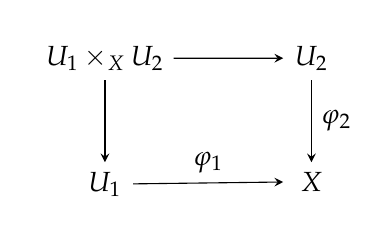
\begin{tikzpicture}
		\matrix (m) [matrix of math nodes,row sep=3em,column sep=4em,minimum width=2em]
		{
			U_1\times_X U_2 & U_2\\ 
			U_1 & X\\};
		\path[-stealth]
		(m-1-1) edge node [above] {} (m-1-2)
		(m-2-1) edge node [above]  {$\varphi_1$} (m-2-2)
		(m-1-1) edge node [right]  {} (m-2-1)
		(m-1-2) edge node [right] {$\varphi_2$} (m-2-2);
	\end{tikzpicture}
	\\
	having the obvious universal property. 
	
\end{definition}
\begin{definition}\label{site_defn}\cite{milne:lec}
	Let  $\mathscr C$  be a category. Suppose that  for each object $U$ of $\mathscr C$ there are  distinguished sets of families of morphisms $\left\{U_\iota \to U\right\}_{\iota\in I}$, called the \textit{coverings} of $U$, 
	satisfying the following axioms: 
	\begin{enumerate}
		\item[(a)] for any covering $\left\{U_\iota \to U\right\}_{\iota\in I}$ and any morphism $U \to V$ in $\mathscr C$, the fibre products 
		$U_\iota\times_U V$ exist, and $\left\{U_\iota\times_U V \to V\right\}_{\iota\in I}$ is a covering of $V$; 
		\item[(b)] if $\left\{U_\iota \to U \right\}_{\iota\in I}$ is a covering of $U$, and if for each $\iota \in I$, $\left\{V_{\iota j} \to U_\iota  \right\}_{j \in I_\iota}$	is a 
		covering of $U_\iota$, then the family $\left\{V_{\iota j }\to U\right\}_{\iota j}$ is a covering of $U$; 
		\item[(c)] for any $U$ in $\mathscr C$, the family $\left\{U\xrightarrow{\Id}U \right\}$ consisting of a single map is a covering of $U$. 
	\end{enumerate}
	The system of coverings is then called a \textit{Grothendieck topology}, and $\mathscr C$  together with 
	the topology is called a \textit{site}. If $\mathbf T$  
	is a site, then $\mathrm{Cat}\left( \mathbf T\right)\bydef \mathscr C$  denotes the underlying category. 
	
\end{definition}
\begin{example}\label{top_gro_exm}
	If $\sX$ is a topological space then one has a category of open subsets and their inclusions. If both $\sU_1, \sU_2 \subset \sX$ are open subsets then one can define a fibre product (cf. Definition \ref{pullback_defn}) by the following way
	$$
\sU_1\times_\sX \sU_2 \bydef \sU_1 \cap \sU_2.	
	$$
	If $\sU \subset \sX$ is an open subset then we assume that a family  $\left\{\sU_\iota \subset \sU\right\}_{\iota\in I}$, is a covering of $\sU$ (cf. Definition \ref{site_defn}) if and only if  $\sU = \cup_{\iota\in I}\sU_\iota$. This system of coverings is a specialization of Grothendieck topology. 
\end{example}
\begin{definition}\label{top_gro_definition}
In the situation of the Example \ref{top_gro_exm} one has a site $\mathbf T_{\sX}$ \textit{arising} from $\sX$.
\end{definition}

\begin{definition}\label{etale_presheaf_defn}\cite{milne:lec}
	A \textit{presheaf of sets} on a site $\mathbf T$ 
	is a contravariant functor $\mathscr F$ from $\mathrm{Cat}\left( \mathbf T\right)$ to the category of sets. Thus,  $\mathscr F$
	to each object $U$ in $\mathrm{Cat}\left( \mathbf T\right)$ 
	attaches a set $\mathscr F\left(U \right)$ , and to each morphism $\varphi: U \to V$
	in $\mathrm{Cat}\left( \mathbf T\right)$, a map $\mathscr F\left(\varphi\right):\mathscr F\left(V \right)\to \mathscr F\left(U \right)$. Note that the notion of a presheaf on $\mathbf T$ 
	does not depend on the 
	coverings. We sometimes denote $\mathscr F\left(\varphi\right)$ by $a \mapsto a|_U$.
	
\end{definition}
Similarly, a presheaf of (Abelian) groups or rings on $\mathbf T$ is a contravariant functor from
$\mathrm{Cat}\left( \mathbf T\right)$ to the category of (Abelian) groups or rings.
\begin{definition}\label{etale_sheaf_defn}\cite{milne:lec}
	A \textit{sheaf} on $\mathbf T$ 
	is a presheaf $\mathscr F$ 
	that satisfies the sheaf condition, that is a sequence 
	\be\label{etale_sheaf_eqn}
	\mathscr F \left(U\right) \to \prod_{\iota \in I} \mathscr F \left(U_\iota \right)\rightrightarrows  \prod_{\iota, j \in I\times I} \mathscr F \left(U_\iota \times_U U_j\right)
	\ee
	is exact for every covering $\left\{U_\iota \to U\right\}$. Thus $\mathscr F$ 
	is a sheaf if the map 
	$$
	f \mapsto \left\{f|_{U_\iota }\right\}:\mathscr F \left(U\right) \to \prod_{\iota \in I} \mathscr F \left(U_\iota \right)
	$$
	identifies $\mathscr F\left( U\right)$ with the subset of the product consisting of families $\left\{f_\iota\right\}$ such that 
	$$
	f_\iota|_{U_\iota \times_U U_j}= f_j|_{U_\iota \times_U U_j}
	$$
	for all $\iota, j \in I$. 
	When $\mathbf T$ 
	is the site arising from a topological space then these definitions coincide with the 
topological ones. 
	
\end{definition}
\begin{definition}\label{forget_sheaf_defn}
There are categories $\mathbf{PreSh}\left(\mathbf T \right)$, $ \mathbf{Sh}\left(\mathbf T\right)$ of presheaves an sheaves. Moreover there is a \textit{forgetful functor} $\mathfrak{Forget} : \mathbf{Sh}\left(\mathbf T \right)\to \mathbf{PreSh}\left(\mathbf T \right)$.
\end{definition}

\begin{statement}\label{site_sheaf_stmt}\cite{johnstone:topos}
	There is an adjoint $\mathfrak{Ass} : \mathbf{PreSh}\left(\mathbf T  \right)\to \mathbf{Sh}\left(\mathbf T \right)$ to the  forgetful functor $\mathfrak{Forget} : \mathbf{Sh}\left(\mathbf T  \right)\to \mathbf{PreSh}\left(\mathbf T \right)$ (cf. Definition \ref{forget_sheaf_defn}).
\end{statement}	
\begin{defn}\label{site_sheaf_ass_defn}\cite{johnstone:topos}
	The given by the Statement  \ref{site_sheaf_stmt} functor $\mathfrak{Ass} : \mathbf{PreSh}\left(\mathbf T  \right)\to \mathbf{Sh}\left(\mathbf T \right)$  is said to be an  \textit{associated sheaf functor}.
\end{defn}
\begin{statement}\label{site_enough_stmt}\cite{johnstone:topos}
	%8.13$
	If $\mathbf T$ is a site then a category $\mathbf {Ab}\left(\mathbf T \right)$ of sheaves of Abelian groups has enough injectives.
\end{statement}
\begin{empt}
	The notion of \textit{topos} is explained in \cite{johnstone:topos}. Any topos is a category. If $\mathbf T$ is a site then a category  $\mathbf{Sh}\left(\mathbf T  \right)$ of sheaves of sets is a topos.
\end{empt}


\begin{definition}\label{grothendiek_topos_defn}\cite{johnstone:topos}
	A topos $\mathscr E$ is said to be a \textit{Grothendieck topos} if there exist a site $\mathbf T$ such that $\mathscr E$ is equivalent to a category  $\mathbf{Sh}\left(\mathbf T  \right)$ of sheaves of sets on $\mathbf T$.
\end{definition}

\begin{definition}\label{geom_mor_defn}\cite{johnstone:topos}
	% 1.16 
	If both $\mathscr E$, $\mathscr F$ are toposes then \textit{geometric morphism} $\mathscr F\xrightarrow{f}\mathscr E$ consists of a pair of functors $\mathscr F\xrightarrow{f_*}\mathscr E$  and $\mathscr E\xrightarrow{f^*}\mathscr F$ (called the \textit{direct} and \textit{inverse images}) such that $f^*$ is left adjoint to $f_*$ and $f^*$ is left exact. 
\end{definition}
%\begin{rem}\label{geom_mor_g_rem}\cite{johnstone:topos}
% 1.16 Grothendieck
%If both $\mathscr E$, $\mathscr F$ are Grothendieck toposes and  $\mathscr F\xrightarrow{f}\mathscr E$ is {geometric morphism} then direct image $f^*$ is left exact. 
%\end{rem}
\begin{definition}\label{constant_presheaf_defn}\cite{johnstone:topos}
If $X$ is an object of $\mathrm{Cat}\left( \mathbf T\right)$ (cf. Definition \ref{site_defn} then for any set $F$ there is a \textit{constant presheaf} $\mathscr P$ such that $\mathscr P\left( U\right) \bydef F$ and $\mathscr P\left( f\right) \bydef \Id_F$ for all $\mathrm{Cat}\left( \mathbf T\right)/X$-morphism $f: U\to V$.
We use a following notation
	\be\label{constant_presheaf_eqn}
	F_X \bydef \mathscr P.
	\ee
\end{definition}


\subsection{Cohomology of sheaves}\label{grothendieck_cohomology_section}
\paragraph{}
Here I follow to \cite{milne:lec}. Let $\mathbf T$ be a site, and let $X$ be an object of $\mathrm{Cat}\left( \mathbf T\right)$. The functor
\bean
\Ga\left(X, \cdot \right) : \mathbf {Ab} \left(\mathbf T \right) \to \mathbf {Ab} ,\\
\mathscr F \mapsto \mathscr F\left(X \right) 
\eean
of global sections is left exact, and we define $H^r\left(X,~ \cdot ~\right)$ to be its $r^{\text{th}}$ right derived functor. Explicitly, for a sheaf $\mathscr F$, choose an injective resolution (cf. Statement \ref{site_enough_stmt})
$$
0 \to \mathscr F \to \mathscr I^0\to \mathscr I^1\to \mathscr I^2 \to ...
$$
and apply the functor $\Ga\left(X, \cdot \right)$ to obtain a complex
\be\label{complex_eqn}
0 \hookto\Ga\left(X,\ \mathscr I^0  \right) \xrightarrow{\dl_0} \Ga\left(X, \mathscr I^1  \right) \xrightarrow{\dl_1} \Ga\left(X, \mathscr I^2  \right) \to ... 
\ee
which is no longer exact (in general). For any $r\ge 0$ the complex \eqref{complex_eqn} yields the $r^{\text{th}}$ \textit{cohomology
group}  
\be\label{etale_coh_eqn}
H^r\left(X,\ \mathscr F \right)\bydef\begin{cases}
	\ker \dl^0 & r = 0\\
 \ker~ \dl_{r} / \im~ \dl_{r - 1}  & r > 0
\end{cases},
\ee
which does not depend on choice of injective resolution up to isomorphism.

\begin{proposition}\label{spectral_sequence_prop}\cite{johnstone:topos}
	%8.17 
	Let $\mathscr F \xrightarrow{f} \mathscr E$ be a geometric morphism (cf. Definition \ref{geom_mor_defn}) between Grothendieck toposes (cf. Definition \ref{grothendiek_topos_defn}). Then
%	\begin{enumerate}		\item [(i)] 
	if $A$ is an Abelian group in $\mathscr E$ then we have a homomorphism $H^q\left(\mathscr E, A \right) \xrightarrow{} H^q \left(\mathscr F, f^*A\right)$ for each $q$ which is functorial in $f$ and natural in $A$.
	%	\item [(ii)] If $B$ is an Abelian group in $\mathscr F$ then we have a spectral sequence (Leray spectral sequence) $H^p\left(\mathscr E, R^qf_*\left(B \right) \right)\Rightarrow H^{p + q}\left(\mathscr F, B \right)$ which is natural in $B$.
%	\end{enumerate}
\end{proposition}
\begin{notation}\label{const_shef_coh_not}
	If  $F$ is an Abelian group and $F_X$ is a {constant presheaf} (cf. Definition \ref{constant_presheaf_defn}) then we use the following notation
	\be\label{const_shef_coh_eqn}
	\forall r\ge 0\quad H^r\left(X, F \right) \bydef H^r\left(X, \mathfrak{Ass} \left( F_X\right)  \right).
	\ee
	where $\mathfrak{Ass}$ means the associated sheaf functor (cf. Definition \ref{site_sheaf_ass_defn}).
\end{notation}




\subsection{\v{C}ech cohomology}\label{presheaf_cohomology_sec}
\paragraph{} Here I follow to \cite{milne:lec}. Let $\mathbf T$ be a site, and let $X$ be an object of $\mathrm{Cat}\left( \mathbf T\right)$. Let $\mathscr U \bydef \left\{U_\iota \to X\right\}_{\iota \in I}$ be  covering of $X$, and let $\mathscr P$ be a presheaf of Abelian groups. Define
\be\label{cech_eqn}
C^r\left( \mathscr U, \mathscr P\right)\bydef \prod_{\left(\iota_0,.... \iota_r\right) \in I^{r+1}} \mathscr P\left(U_{\iota_0,.... \iota_r} \right)\quad \text{where} \quad U_{\iota_0,.... \iota_r} \bydef U_{\iota_0}\times_X...\times_XU_{\iota_r}. 
\ee
For $s \in C^r\left( \mathscr U, \mathscr P\right)$ define $d^rs \in C^{r+1}\left( \mathscr U, \mathscr P\right)$ by the rule
$$
d^rs_{\iota_0,..., \iota_{r + 1}}\bydef \sum_{j = 0}^{r + 1}\left(-1 \right) \mathrm{res}_j\left(s_{\iota_0,..., \iota_{j-1},...,\iota_{j+1},..., \iota_{r + 1}} \right)  
$$
$\mathrm{res}_j$ is the restriction map corresponding to the projection map
$$
U_{\iota_0,..., \iota_{r + 1}}\mapsto U_{\iota_0,..., \iota_{j-1},...,\iota_{j+1},.., \iota_{r + 1}}.
$$
As in the classical case, one verifies by a straightforward calculation that
$$
C^\bullet\left( \mathscr U, \mathscr P\right) \bydef C^0\left( \mathscr U, \mathscr P\right) \to C^r\left( \mathscr U, \mathscr P\right) \xrightarrow{d_r} C^r\left( \mathscr U, \mathscr P\right)\to ...
$$
is a complex. Define
\be\label{cech_coh_eqn}
\check{H}^r\left( \mathscr U, \mathscr P\right) \bydef H^r\left(C^\bullet\left( \mathscr U, \mathscr P\right)   \right)= \begin{cases}
\ker d_0 & r = 0\\
\ker d_r / \im d_{r-1} & r > 0
\end{cases}. 
\ee
It is called the $r^{\text{th}}$ \textit{\v{C}ech cohomology group} of $\mathscr P$ relative to the covering $\mathscr U$.
Note that
$$
\check{H}^0\left( \mathscr U, \mathscr P\right)= \ker\left(\prod \mathscr P_\iota \rightrightarrows \prod \mathscr P_{\iota,j} \right) 
$$
Therefore, for a sheaf $\mathscr F$ one has
$$
\check{H}^0\left( \mathscr U, \mathscr F\right)=\Ga\left( \mathscr U, \mathscr F\right).
$$
A second covering $\mathscr V \bydef \left\{V_j\to X \right\}_{j \in J}$ of $X$ is called a \textit{refinement} of $\mathscr U$ if there is a
map $\tau : J\to I$ such that $V_j \to X$ factors through $U_{\tau_j}\to X$ for all $j \in J$ . The choice of
a $\tau$ and $X$-morphisms $\varphi_{j}: V_j \to U_{\tau_j}$ for each $j$ determines a map of complexes
\bean
\tau^\bullet: C^\bullet\left( \mathscr U, \mathscr P\right)\to C^\bullet\left( \mathscr V, \mathscr P\right),\\
\left( \tau^r s_{j_0,..., j_{r}} \right) \bydef s_{\tau j_0,..., \tau j_{r}}.
\eean
As in the classical case, one verifies that the map on cohomology groups
$$
\rho \left(\mathscr U, \mathscr V \right): \check{H}^r\left( \mathscr U, \mathscr P\right)\to \check{H}^r \left( \mathscr V, \mathscr P\right)
$$
is independent of all choices. We may pass to the limit over all coverings, and so obtain limits
\be\label{chech_eqn}
\check{H}^r\left(X, \mathscr P\right)\bydef \varinjlim_{\mathscr U}\check{H}^r\left( \mathscr U, \mathscr P\right).
\ee

\begin{defn}\label{chech_defn}\cite{bryl:loop,milne:lec}
	The  \textit{\v{C}ech cohomology groups} are given by equation \eqref{chech_eqn}.
\end{defn}
These groups  have the following properties:
\begin{enumerate}
	\item [(a)] $\check{H}^0\left(X, \mathscr F\right)= \Ga\left( X, \mathscr F\right)$ for any sheaf $\mathscr F$ on $X$;
	\item[(b)] $\check{H}^r\left(X, \mathscr I\right)$, $r > 0$, for all injective sheaves $\mathscr I$
\end{enumerate}
(cf \cite{milne:lec} for details).
\begin{empt}
	For any Abelian group $F$ one can define a constant presheaf $F_X$ of Abelian groups (cf. Definition \ref{constant_presheaf_defn}). 
	We use a following notation
	\be\label{etale_hom_a_eqn}
	\check{H}^r\left(X, F\right)\bydef \check{H}^r\left(X, F_X\right).
	\ee
\end{empt}
\subsection{Grothendieck topology of $C^*$-algebras }
\paragraph*{}

If $A$ is a $C^*$-algebra then there is a category $\mathbf{Hered}/A$ such that:
\begin{itemize}
	\item $\mathbf{Hered}/A$-objects are hereditary $C^*$- subalgebras of $A$,
	\item $\mathbf{Hered}/A$-morphism  from $B' \subset A$ to $B'' \subset A$ is a natural inclusion $B'\subset B''$ such that a following diagram 
	\newline
	\begin{tikzpicture}
		\matrix (m) [matrix of math nodes,row sep=3em,column sep=4em,minimum width=2em]
		{
			B'  &  & B''\\ 
			& A &\\};
		\path[-stealth]
		(m-1-1) edge node [above] {$\subset$} (m-1-3)
		(m-1-1) edge node [above]  {} (m-2-2)
		(m-1-3) edge node [right]  {} (m-2-2);
	\end{tikzpicture}
	\\
	is commutative.
\end{itemize}
For any two $\mathbf{Hered}/A$-objects $B', B''$ we define their \textit{fibre product} (cf. Definition \ref{pullback_defn}) by the following way
$$
B'\times_A B'' \bydef B'\cap B''.
$$

\begin{definition}\label{hered_cov_defn}
	For any $\mathbf{Hered}/A$-object $B$ a distinguished set of families of inclusions $\left\{B_\iota \subset B\right\}_{\iota\in I}$, called a \textit{covering} of $B$ if $B$ is a generated by the union $\cup B_\iota$ hereditary $C^*$-subalgebra of $A$ (cf. Definition \ref{hered_gen_defn}).
\end{definition}

\begin{lemma}\label{grothendieck_ca_lem}
	A given by the Definition \ref{hered_cov_defn} system of coverings satisfies to  the Definition \ref{site_defn}, so one has a natural Grothendieck topology.
\end{lemma}
\begin{proof}
	If $A$ be a $C^*$-algebra, then one needs check that hereditary $C^*$-subalgebras of $A$ satisfy to axioms (a)-(c) of the Definition \ref{site_defn}.\\
	(a) Let $B, C\subset A$ be subalgebras. A covering of $B$ is a family $\left\{B_\iota\subset B\right\}_{\iota \in I}$ of subalgebras of $B$ such that $B$ is a generated by a union $\bigcup B_\iota$ hereditary $C^*$-subalgebra (cf. Definition \ref{hered_gen_defn}). If  $L\left( B\right)$, $L\left( C\right)$ and $L\left( B_\iota \right)$ are given by the equation \eqref{left_ideal_eqn} closed left ideals then $L\left(B\cap C \right) = L(B)\cap L(C)$, $~L\left(B_\iota \cap C \right)= L\left(B_\iota \right)\cap L\left( C \right)$ (cf. Lemma \ref{hered_ideal_lem}). Moreover $L\left(B\right)$ is the $C^*$-norm closure of an algebraic sum $\sum_\iota L\left( B_\iota\right)$. For any $\iota \in I$ one has $L\left(B_\iota\right)\cap L\left(C\right)\subset L\left(B\right)\cap L\left(C\right)$ it follows that $\sum_\iota \left( L\left(B_\iota\right)\cap L\left(C\right)\right) \subset L\left(B\right)\cap L\left(C\right)$. Since the left ideal  $L\left(B\right)\cap L\left(C\right)$ is $C^*$-norm closed the $C^*$-norm closure of an algebraic sum $\sum_\iota \left( L\left(B_\iota\right)\cap L\left(C\right)\right)$ is a subset of  the intersection $L\left(B\right)\cap L\left(C\right)$ i.e. a generated by a union $\cup_\iota \left( B_\iota\cup C\right)$ hereditary subalgebra is a subalgebra of the intersection $B\cap C$. If $\eps > 0$ and $ b\in L\left(C\right)\cap L\left(B\right)$ then from the from the Theorem \ref{left_ideal_thm} it follows that there is a positive $u \in L\left(C\right)$ such that 
	\bean
	\left\|u \right\| \le 1,\\
	\left\|b - b u\right\|< \frac{\eps}{2}.
	\eean 
	There is a sum $\sum_{k = 1}^n b_{k}$ such that
	\bean
	\forall k\in \{1,..., n\}\quad \exists \iota_k\in I \quad b_k \in L\left( B_{\iota_k}\right)  ,\\
	\left\|b - \sum_{k = 1}^n b_k \right\|< \frac{\eps}{2}.
	\eean
	Applying the triangle identity one has
	$$
	\left\|b -  \left( \sum_{k = 1}^n b_k\right)  u\right\|	\le 	\left\|\left( b -   \sum_{k = 1}^n b_k\right)  u\right\|+ \left\|b -   b  u\right\|< \left\| b -   \sum_{k = 1}^n b_k\right\|\left\|  u\right\|+ \frac{\eps}{2}< \eps.
	$$
	From the following circumstances:
	\begin{itemize}
		\item  the number $\eps$ is arbitrary small,
		\item $\left( \sum_{k = 1}^n b_k\right)  u\in \sum_\iota \left( L\left(B_\iota\right)\cap L\left(C\right)\right)$
	\end{itemize}
	we conclude that $b$ lies in the $C^*$-norm closure of $\sum_\iota \left( L\left(B_\iota\right)\cap L\left(C\right)\right)$. So $L\left(B\right)\cap L\left(C\right)$ equals to the $C^*$-norm closure of $\sum_\iota \left( L\left(B_\iota\right)\cap L\left(C\right)\right)$ and $B\cup C$ is a generated by $\cup_\iota \left(B_\iota\cap C \right)$ hereditary $C^*$-algebra. Thus 
	a family $\left\{B_\iota\cap C \subset B\cap C\right\}_{\iota\in I}$ is a {covering} of $B\cap C$ (cf. Definition \ref{hered_cov_defn}).
	\\
	(b) If a family $\left\{B_\iota\subset B\right\}_{\iota\in I}$ is a covering of $B$ and for all $\iota$ a family $\left\{C_{\iota j}\subset B_\iota \right\}_{j\in J_\iota}$ is a covering of $B_\iota$ then  one has:
	\begin{itemize}
		\item The given by the equation \eqref{left_ideal_eqn}  closed left ideal $L\left( B\right)$ is the $C^*$-norm closure of an algebraic sum  $\sum_\iota L\left( B_\iota \right)$ 
		\item for all $\iota\in I$ the left ideal  $L\left( B_\iota \right)$ is  the $C^*$-norm closure of an algebraic sum  $\sum_{j\in J_\iota} L\left( C_{\iota j} \right)$.
	\end{itemize}
	From $\sum_\iota L\left( B_\iota \right)\subset L\left(B \right)$ and $\sum_j L\left( C_{\iota_j} \right)\subset L\left(B_\iota \right)$ for any $\iota \in I$ it follows that $\sum_{\iota j} L\left( C_{\iota_j} \right)\subset L\left(B \right)$. However the ideal $ L\left(B \right)$ is $C^*$-norm closed so a $C^*$-norm closure of $\sum_{\iota j} L\left( C_{\iota_j} \right)$ is a subset of $ L\left(B \right)$. 
	For all $b \in L\left( B\right)$ and  $\eps > 0$	there is a sum $\sum_{k = 1}^n b_{k}$ such that
	\bean
	\forall k\in \{1,..., n\}\quad \exists \iota_k\in I \quad b_k \in L\left( B_{\iota_k}\right) ,\\
	\left\|b - \sum_{k = 1}^n b_k \right\|< \frac{\eps}{2}.
	\eean
	For all $k \in \{1,...,n\}$ there is a sum $\sum_{l = 1}^{m_k} c_{k l}$ such that
	\bean
	\forall l\in \{1,..., {m_k}\}\quad \exists j_l \in J_\iota  \quad c_l \in L\left( C_{\iota_k j_l}\right) ,\\
	\left\|b_k - \sum_{l = 1}^{m_k} c_{\iota l} \right\|< \frac{\eps}{2n}.
	\eean
	From these facts it follows that if
	$$
	b' \bydef \sum_{k = 1}^n \sum_{l = 1}^{m_k} c_{k l}
	$$
	then
	\bean
	b' \in \sum_{\iota j} L\left( C_{\iota j}\right) ,\\
	\left\|b - b' \right\| < \eps.
	\eean	
	The element $b$ lies in the $C^*$-norm closure of the algebraic sum $\sum_{\iota j}L\left(  C_{\iota j}\right) $ because the number $\eps$ is arbitrary small, so $L\left(B \right)$ is the $C^*$-norm closure of the algebraic sum $\sum_{\iota j}L\left(  C_{\iota j}\right)$. Taking into account  the Lemma \ref{hered_ideal_lem} one can deduce that $B$ is a generated by a union $\cup_{\iota j}  C_{\iota j}$ hereditary subalgebra (cf. Definition \ref{hered_gen_defn}), i.e. 
	a family $\left\{C_{\iota j} \subset B\right\}$ is a {covering} of $B$.
	\\
	(c) Evident.
\end{proof}



\begin{definition}\label{grothendieck_ca_defn}
	The given by the Lemma \ref{grothendieck_ca_lem} Grothendieck topology  is said to be an  $A$-\textit{topology}. A corresponding  site (cf. Definition \ref{site_defn}) $\mathbf{T}_A$ is said to be \textit{arising} from $A$ (cf. Definition \ref{top_gro_definition}).
\end{definition}
\begin{remark}
	For any locally compact Hausdorff space $\sX$ there is a one to one correspondence between open subsets of $\sX$ and hereditary subalgebras of $C_0\left(\sX\right)$, So an arising from $\sX$ site $\mathbf{T}_\sX$ (cf. Definition \ref{top_gro_definition}) is naturally equivalent to a site $\mathbf{T}_{C_0\left( \sX\right) }$ arising from $C_0\left( \sX\right)$ (cf. Definition \ref{grothendieck_ca_defn}). It follows that described here theory is a generalization of the theory of sheaves on topological spaces.
\end{remark}
\begin{lemma}\label{min_lem}
	Let $A$ be a $C^*$-algebra, and let $B$ be a hereditary $C^*$-subalgebra of $A$. If $B$ is generated by a family $\left\{B_\iota \subset A\right\}_{\iota \in I}$ of hereditary $C^*$-subalgebras then $L\left(B\right)$ is a minimal closed left ideal containing an algebraic sum $\sum_{\iota\in I} L\left(B_\iota \right)$ where $L\left(B\right)$ and  $L\left(B_\iota \right)$ are given by the equation \eqref{left_ideal_eqn}. Equivalently $L\left(B\right)$ is the intersection of all containing the sum $\sum_{\iota\in I} L\left(B_\iota \right)$  closed left ideals of $A$.
\end{lemma}
\begin{proof}
	From $L\left(B_\iota \right)\subset L\left(B\right)$ for all $\iota\in I$ it follows that $\sum_{\iota\in I} L\left(B_\iota \right)\subset L\left(B\right)$. Since $L\left(B\right)$ is $C^*$-norm closed the $C^*$-norm closure of $\sum_{\iota\in I} L\left(B_\iota \right)$ is a subset of $L\left(B\right)$. If a left $L$-ideal is $C^*$-norm closure of $\sum_{\iota\in I} L\left(B_\iota \right)$ and $L\subsetneqq L\left(B\right)$ then one has:
	\begin{itemize}
		\item an intersection  $L\cap L^*$ is a hereditary $C^*$-subalgebra of $A$ (cf. Lemma \ref{hered_ideal_lem}),
		\item $\cup_{\iota\in I}B_\iota\subset L\cap L^*$.
	\end{itemize}
	From these circumstances it follows that a generated by the union $\cup_{\iota\in I}B_\iota$ hereditary algebra is a subalgebra of $L\cap L^*$. This fact contradicts with $L\subsetneqq L\left(B\right)$, so $L\left(B\right)$ is a minimal closed left ideal containing an algebraic sum $\sum_{\iota\in I} L\left(B_\iota \right)$. From this fact it follows that $L\left(B\right)$ is the intersection of all containing the sum $\sum_{\iota\in I} L\left(B_\iota \right)$  closed left ideals of $A$.
\end{proof}
If $A$ is a  $C^*$-algebra $A$ the one has
\be\label{four_decompositon_eqn}
\forall a \in A\quad \exists a_1, a_2, a_3, a_4 \in A_+\quad a=a_1 - a_2 + ia_3 - ia_4
\ee
where $a_1, a_2, a_3, a_4$ are positive.
\begin{empt}\label{hered_repr_p_empt}
	Let $\rho: A\hookto B\left(\H \right)$ be a faithful nondegenerate representation (cf. Definitions \ref{faithful_repr_defn} and \ref{nondegenerate_repr_defn}).
	If $B$ is a hereditary subalgebra of $A$ (cf. Definition \ref{hered_defn}), and   $\left\{u_\la \right\}_{\la \in \La} \subset  B_+$ is an  approximate unit of $B$ (cf. Definition \ref{approximate_unit_defn}) then
	one has
	\be\label{hered_uau_eqn}
	\begin{split}
		%	\bt\text{-}\lim_\la u_\la = 1_{ M\left( B\right) },\\
		B = \left\{ a \in A \left|~\lim_{\la\in\La} \left\| a - u_\la a u_\la\right\|= 0 \right.\right\}.
	\end{split}
	\ee
	From the Lemma \ref{increasing_convergent_w_lem} it turns out that the net $\left\{\rho\left( u_\la\right)  \right\}$  is convergent  with respect to the strong topology of $B\left(\H \right)$ (cf. Definition \ref{strong_topology_defn}). If $p \bydef s$-$\lim\rho\left(  u_\la \right) \in B\left( \H\right)$ is a strong limit then from the proof of the Lemma \ref{hered_repr_lem}  it follows that $p$ is a projection onto the norm completion of $\rho\left(B\right)\H$.
	From \eqref{hered_uau_eqn} it turns out that 
	\be\label{hered_pap_eqn}
	B = \left\{ a \in A | p\rho\left( a\right) p = \rho \left( a\right)\right\}
	\ee
	and  there is a natural representation
	\be\label{hered_rep_eqn}
	B \hookto B\left(p \H \right) 
	\ee
\end{empt}
\begin{lemma}\label{hered_full_lem} 
	In the situation \ref{hered_repr_p_empt} the representation \eqref{hered_rep_eqn} is  faithful.
\end{lemma}
\begin{proof}
	For any $a \in B$ there is $\xi \in \H$ such that $\rho\left(a\right)\xi \neq 0$. From  \eqref{hered_rep_eqn} it follows that $\rho\left( a\right) \xi = p \rho\left( a\right) p\xi \neq 0$, so $\rho\left( a\right) p\xi \neq 0$. On the other hand $p\xi \in p\H$.
\end{proof}

\begin{lemma}\label{hered_nondegenerate_lem} 
	In the situation \ref{hered_repr_p_empt} the representation \eqref{hered_rep_eqn} is  nondegenerate.
\end{lemma}
\begin{proof}
	For any $\xi \in p\H\setminus\{0\}$ there is $a \in A$ such that $a \xi \neq 0$. From the equation \eqref{four_decompositon_eqn} we can suppose that $a$ is positive. If  $\left\{u_\la \right\}_{\la \in \La} \subset  B_+$ is an  approximate unit of $B$ (cf. Definition \ref{approximate_unit_defn}) then from $p=s$-$\lim u_\la$ one   has a norm limit $\lim_{\la \in \La}u_\la \xi = \xi$, it follows that  $\lim_{\la \in \La}a u_\la \xi = a\xi$. There is $\la_0\in \La$ such that $a u_{\la_0} \xi \neq 0$, so one has
	\bean
	\left(a u_{\la_0} \xi, a u_{\la_0} \xi \right) = \left(\xi , \left( u_{\la_0} a^*a u_{\la_0}\right) \xi  \right)\neq 0\quad \Rightarrow \quad \left(  u_{\la_0} a^*a u_{\la_0}\right) \xi	\neq 0.
	\eean
	However $ u_{\la_0} a^*a u_{\la_0}\in B$.
\end{proof}
\begin{lemma}\label{hered_repr_p_lem}
	In the situation \ref{hered_repr_p_empt} if $\pi: A\to B\left(\H \right)$ is an atomic  representation (cf. Definition \ref{atomic_repr_defn}) then the given by \eqref{hered_rep_eqn} representation $ B \hookto B\left(p \H \right)$ is atomic.
\end{lemma}
\begin{proof}
	One can prove this lemma by an application of the proof of the Lemma 
	\ref{hered_repr_lem}.
\end{proof}





\section{Topological presheaves and sheaves}
\subsection{General theory}
\paragraph{}
The explained below definitions are specializations of   \ref{etale_presheaf_defn} and  \ref{etale_sheaf_defn} ones (cf. Example \ref{top_gro_exm}).
\begin{definition}\label{presheaf_defn}\cite{hartshorne:ag}
	Let $\sX$ be a topological space. A \textit{presheaf} $\mathscr F$ of Abelian groups on  $\sX$ consists of the data:
	\begin{itemize}
		\item[(a)] for every open subset $\sU \subseteq \sX$, an Abelian group $\mathscr F\left(\sU\right)$, and 
		\item[(b)] for every inclusion $\sV \subseteq \sU$ of open subsets of $\sX$, a morphism of Abelian groups $\rho_{\sU \sV}:\mathscr F\left(\sU\right) \to \mathscr F\left(\sV\right)$,\\
		subject to conditions
		\begin{itemize}
			\item [(0)] $\mathscr F\left(\emptyset \right)= 0$, where $\emptyset$ is the empty set,
			\item[(1)] $\rho_{\sU \sU}$ is the identity map, and
			\item[(2)] if $\mathcal W \subseteq \sV \subseteq \sU$ are three open sets, then $\rho_{\sU \mathcal W} = \rho_{\sV \mathcal W }\circ \rho_{\sU \sV}$.
		\end{itemize}
	\end{itemize}
\end{definition}

\begin{definition}\label{sheaf_defn}\cite{hartshorne:ag}
	A \textit{presheaf} $\mathscr F$ on  
	a topological space $\sX$ is a \textit{sheaf}  if it satisfies the following supplementary conditions:
	\begin{itemize}
		\item[(3)] If $\sU$ is an open set, and if $\left\{\sV_{\a}\right\}$ is an open covering of $\sU$, and if $s \in \mathscr F\left(\sU\right)$ is an element such that $\left.s\right|_{\sV_{\a}}= 0$ for all $\a$, then $s = 0$;
		\item[(4)] If $\sU$ is an open set, if $\left\{\sV_{\a}\right\}$ is an open covering of $\sU$ (i.e. $\sU = \cup\sV_\a$), and we have elements $s_\a$ for each $\a$, with property that for each $\al, \bt, \left.s_\a\right|_{\sV_{\a}\cap \sV_{\bt}}= \left.s_\bt\right|_{\sV_{\a}\cap \sV_{\bt}}$, then there is an element $s \in \mathscr F\left(\sU\right)$ such that $\left.s\right|_{\sV_\a} = s_\a$ for each $\a$.
	\end{itemize}
	(Note condition (3) implies that $s$ is unique).
\end{definition}



%\begin{definition}
%	A presheaf \ref{top_x_sheaf_defn} satisfying (4) of the Definition \ref{sheaf_defn} is called \textit{conjunctive} (for $\sU$). (cf. \cite{bredon:sheaf})
%\end{definition}
\begin{definition}\label{stalk_defn}\cite{hartshorne:ag}
	If $\mathscr F$ is a {presheaf} on $\sX$, and if $x$ is a point of $\sX$ we define the \textit{stalk} or the \textit{germ} $\mathscr F_x$ of $\mathscr F$ at $x$ to be the direct limit of groups $\mathscr F\left(\sU\right)$ for all open sets $\sU$ containing $x$, via restriction maps $\rho$.
\end{definition}

\begin{prdf}\label{sheaf_prdf}\cite{hartshorne:ag}
	Given a presheaf $\mathscr F$, there is a sheaf  $\mathscr F^+$ and a morphism $\th: \mathscr F \to \mathscr F^+$, with the property that for any sheaf  $\mathscr G$, and any morphism $\varphi: \mathscr F \to \mathscr G$, there is a unique morphism $\psi:\mathscr F^+\to \mathscr G$ such that $\varphi = \psi \circ \th$. Furthermore the pair $\left(\mathscr F^+, \th\right)$ is unique up to unique isomorphism. $\mathscr F^+$ is called the $\mathrm{sheaf~associated}$ to the presheaf $\mathscr F$. 
\end{prdf}
\begin{remark}
	The above Proposition is a specialization of the Statement \ref{site_enough_stmt}.
\end{remark}

\begin{exercise}\label{sheaf_etale_exer}\cite{hartshorne:ag}
	%1.13. 
	\textit{
		\'Espace Etal\'e of a Presheaf}. %(This exercise is included only to establish the connection between our definition of a sheaf and another definition often found in the literature. See for example Godement [1, Ch. II, �1.2].)
	Given a presheaf $\mathscr F$ on $\sX$, we define a topological space $\mathrm{Sp\acute{e}}\left(\mathscr F \right)$ , called the \textit{
		\'espace etal\'e} of a presheaf of $\mathscr F$ as 
	follows. As a set, $\mathrm{Sp\acute{e}}\left(\mathscr F \right)= \bigcup_{x\in\sX} \mathscr F_x$. We define a projection map $p: \mathrm{Sp\acute{e}}\left(\mathscr F \right)\to \sX$
	by sending $s_x\in \mathscr F_x$ to $x$. For each open set $\sU\subset\sX$ and each section $s\in \mathscr F\left(\sU \right)$  we 
	obtain a map: $\overline{s}: \sU \to  \mathrm{Sp\acute{e}}\left(\mathscr F \right)$ by sending $x \mapsto s_x$, its stalk at $x$. This map has the property that 
	$p\circ \overline{s}= \Id_\sX$, in other words, it is a "section" of $p$ over $\sU$. We now 
	make $\mathrm{Sp\acute{e}}\left(\mathscr F \right)$ into a topological space by giving it the strongest topology such that 
	all the maps $\overline{s}: \sU \to  \mathrm{Sp\acute{e}}\left(\mathscr F \right)$ for all $\sU$ and all $s\in \mathscr F\left(\sU \right)$ , are continuous. Now 	show that the sheaf $\mathscr F^+$ associated to $\mathscr F$ can be described as follows: for any 
	open set $\sU\subset \mathscr F$, $\mathscr F\left(\sU \right)$ is the set of continuous sections of $\mathrm{Sp\acute{e}}\left(\mathscr F \right)$ over $\sU$. In 
	particular, the original presheaf $\mathscr F$ was a sheaf if and only if for each $\sU\subset \sX$,  $\mathscr F\left(\sU \right)$ is 
	equal to the set of all continuous sections of $\mathrm{Sp\acute{e}}\left(\mathscr F \right)$ over $\sU$. 
\end{exercise}	
\begin{exercise}\label{sheaf_etale_open_exer}

Let $s \in \mathscr F\left(\sU\right)$ be a section. Prove following statements.
\begin{enumerate}
	\item The set 
	\be\label{sheaf_u_s_eqn}
\mathscr U_s\bydef \left\{s_x\right\}_{x \in \sU}
	\ee
is open subset  of the \'espace etal\'e  of $\mathrm{Sp\acute{e}}\left(\mathscr F \right)$ of the presheaf $\mathscr F$.
	\item The family  of all given by the equation \eqref{sheaf_u_s_eqn} sets $\mathscr U_s$ is basis of the topology of  $\mathrm{Sp\acute{e}}\left(\mathscr F \right)$.
	\item The natural continuous map $\mathrm{Sp\acute{e}}\left(\mathscr F \right)\to\sX$ is local homeomorphism.
	\end{enumerate}
\end{exercise}

\begin{definition}\label{sheaf_inv_im_defn}\cite{hartshorne:ag}
	Let $f: \sX\to \sY$ be a continuous map of topological spaces. For any sheaf  $\mathscr F$ on $\sX$, we define the \textit{direct image} sheaf  $f_*\mathscr F$ on $\sY$ by $\left(f_*\mathscr F\right)\left(\sV\right)= \mathscr F\left(f^{-1}\left(\sV\right)\right)$ for any open set $\sV \subseteq \sY$. For any sheaf  $\mathscr G$ on $\sY$, we define the \textit{inverse image} sheaf  $f^{*}\mathscr G$ on $\sX$ be the sheaf  associated to the presheaf  $\sU \mapsto \lim_{\sV \supseteq f\left(\sU\right)} \mathscr G\left(\sV\right)$, where $\sU$ is any open set in $\sX$, and the limit is taken over all open sets $\sV$ of $\sV$ containing $f\left(\sU\right)$.
\end{definition}

\begin{remark}\label{geometric_morphism_rem}\cite{johnstone:topos}
	%1.17
	If $f : \sX \to \sY$ is a continuous map then a given by the Definition \ref{sheaf_inv_im_defn} pair  of functors $f_*$ and $f^{*}$ rise a geometric morphism (cf. Definition \ref{geom_mor_defn}) $\mathbf{Sh}\left(\sX\right)\to \mathbf{Sh}\left(\sY\right)$ between categories of sheaves. 
\end{remark}
\begin{exercise}\label{dir_image_exer}
	Let $f : \sX \to \sY$ be a continuous map, and let $F$ be a set. Prove that if  	both $F_\sX$ and $F_\sY$ are constant presheaves  (cf. Definition \ref{constant_presheaf_defn}) on $\sX$ and $\sY$ 
	then one has:
	\begin{enumerate}
		\item there is a natural isomorphism of sheaves
		\bean\label{dir_image_eqn}
		\mathfrak{Ass}\left( F_\sY\right) \cong f_*\mathfrak{Ass}\left( F_\sX\right)
		\eean
		where 
		$\mathfrak{Ass}$  means the associated sheaf functor (cf. Definition \ref{site_sheaf_ass_defn}) and 	
		$f_*$ means the direct image (cf. Definition \ref{sheaf_inv_im_defn}),
		\item if $f$ ia a local homeomorphism then there is a natural isomorphism of sheaves
		\be\label{inv_image_eqn}
		\mathfrak{Ass}\left( F_\sX\right) \cong f^*\mathfrak{Ass}\left( F_\sY\right)
		\ee
	where	$f^*$ means the  inverse image (cf. Definition \ref{sheaf_inv_im_defn}).
	\end{enumerate}
	

	
\end{exercise}
\subsection{Cohomology}
\paragraph{}
The described below theories are specializations of described in sections \ref{grothendieck_cohomology_section} and \ref{presheaf_cohomology_sec} ones (cf. Example \ref{top_gro_exm}).
%\begin{lemma}\cite{hartshorne:ag}
%	Let $\sX$ be a topological space, and $\mathscr U$ an open covering of $\sX$. Then for any sheaf $\mathscr U$ on $\sX$ and	for each $r \ge 0$ there is a natural map, functorial in $\mathscr F$.
%	$$
%	\check{H}^r\left(\mathscr U, \mathscr F \right) \to H^r\left( \sX, \mathscr F\right) 
%	$$
%	where both $\check{H}^r$ and $H^r$ are given by the equations \eqref{cech_coh_eqn} and \eqref{etale_coh_eqn} respectively.
%\end{lemma}
%\begin{remark}
%From the above lemma and the equation  \ref{chech_eqn} for each $r\ge 0$ one has a homomorphism
%$$
%\check{H}^r\left(\sX, \mathscr F \right) \to H^r\left( \sX, \mathscr F\right).
%$$
%\end{remark}
\begin{empt}
	If $f: \sX\to\sY$ is a continuous map  $\mathscr U = \left\{\sU_\iota\right\}_{\iota} \in I$ is a covering of $\sY$ (cf. Definition \ref{site_defn} and Example \ref{top_gro_exm}) then a family $f^{-1}\left(\mathscr U \right) \bydef \left\{f^{-1}\left( \sU_\iota\right) \right\}_{\iota} \in I$ is a covering of $\sX$. Let $F$ be a Abelian group, and let $F_\sX$, $F_\sY$ be a corresponding constant presheaves (cf. Definition \ref{constant_presheaf_defn}) on $\sX$ and $\sY$.  Following equation
	\be\label{top_cech_eqn}
	C^r\left( \mathscr U,  F_\sY\right)\bydef \prod_{\left(\iota_0,.... \iota_r\right) \in I^{r+1}}  F_\sY\left(\sU_{\iota_0,.... \iota_r} \right)\quad \text{where} \quad \sU_{\iota_0,.... \iota_r} \bydef \sU_{\iota_0}\cap...\cap \sU_{\iota_r}. 
	\ee
	is a specialization of \eqref{cech_eqn} one (cf. Example \ref{top_gro_exm}). For any $\left(\iota_0,.... \iota_r\right) \in I^{r+1}$ one has an isomorphism
	$$
	F_\sY\left(\sU_{\iota_0,.... \iota_r} \right)\cong F_\sX\left(f^{-1}\left( \sU_{\iota_0,.... \iota_r} \right)\right) \cong F.
	$$
	Above isomorphisms yield an isomorphism
	$$
	C^r\left( \mathscr U, F_\sY\right)\xrightarrow{\approx} C^r\left( f^{-1}\left( \mathscr U\right) , F_\sX\right)
	$$
    So there is an isomorphism
    $$
 \varinjlim_{\mathscr U}\check{H}^r\left( \mathscr U, F_\sY\right)\xrightarrow{\approx}\varinjlim_{\mathscr U}\check{H}^r\left(f^{-1}\left(  \mathscr U\right) , F_\sX\right).
    $$
On the other hand from   \eqref{chech_eqn}  it follows that there are homomorphisms
\bean
\check{H}^r\left(f^{-1}\left(  \mathscr U\right) , F_\sX\right)\to \check{H}^r\left(\sX , F_\sX\right),\\
\varinjlim_{\mathscr U} \check{H}^r\left(f^{-1}\left(  \mathscr U\right), F_\sX\right)\to \check{H}^r\left(\sX , F_\sX\right)
\eean
so one has a homomorphism
$$
\varinjlim_{\mathscr U} \check{H}^r\left(  \mathscr U, F_\sY\right)\to \check{H}^r\left(\sX , F_\sX\right)
$$
and applying \eqref{chech_eqn} one can obtain a natural homomorphism
	$$
	\check{H}^r\left(f\right):\check{H}^r\left(\sY, F_\sY \right)\to \check{H}^r\left(\sX, F_\sX \right)\quad r \ge 0.
	$$
	The details of the construction of the homomorphism $\check{H}^r\left(f\right)$  are explained in \cite{eust}. Using the Notation \ref{constant_presheaf_defn} one has homomorphisms
	\be\label{cech_hom_eqn}
	\begin{split}
		\check{H}^r\left(f\right):\check{H}^r\left(\sY, F \right)\to \check{H}^r\left(\sX, F \right)\quad r \ge 0,\\
		\check{H}^\bullet\left(f\right):\check{H}^\bullet\left(\sY, F \right)\to \check{H}^\bullet\left(\sX, F \right).
	\end{split}
	\ee
	If both $\sX \xrightarrow{f}\sY$ and $\sY \xrightarrow{g}\sZ$ are continuous maps then from this construction it turns out that
	\be\label{cech_hom_comp_eqn}
	\begin{split}
		\check{H}^\bullet\left(g\circ f\right)= \check{H}^\bullet\left( f\right)\circ \check{H}^\bullet\left(g\right):\check{H}^\bullet\left(\sZ, F \right)\to \check{H}^\bullet\left(\sX, F \right)
	\end{split}
	\ee
	
\end{empt}

\begin{empt}\label{tens_prop_c_empt}\cite{bryl:loop}
\v{C}ech cohomology has the advantage of allowing an easy and explicit construction of a \textit{cup}-\textit{product}
$$
\check{H}^p\left(\mathscr U,  \mathscr F\right) \otimes \check{H}^q\left(\mathscr U,  \mathscr G\right)\to \check{H}^p\left(\mathscr U,  \mathscr F\otimes \mathscr G\right).
$$
		Here $\mathscr F$ and $\mathscr G$ are sheaves of Abelian groups on $\sX$, and the \textit{tensor product}-\textit{sheaf}
	 $\mathscr F\otimes \mathscr G$ is the sheaf associated to the presheaf $\sU \mapsto \mathscr F(\sU)\otimes \mathscr G(\sU)$. The 
		stalk (cf. Definition \ref{stalk_defn}) at $x$ of $\mathscr F\otimes \mathscr G$ is $\mathscr F_x\otimes \mathscr G_x$. The cup-product will be defined from a 
		morphism of complexes. We first need the notion of tensor product $A^\bullet \otimes  B^\bullet$
		of two complexes; this is the total complex of the double complex $A^\bullet \otimes  B^\bullet$. 
		So the degree $n$-term of $A^\bullet \otimes  B^\bullet$ is $\oplus A^p\otimes B^{n-p}$. The differential in $A^\bullet \otimes  B^\bullet$  
		is 
		$$
	d \left(a \otimes b\right)	\bydef \left(da\right)\otimes b + \left(-1\right)^p a \otimes db
		$$
		
	for $a\in A^p$, $b \in B^q$. We have the obvious 
		map 
	$$
\otimes :H^p\left(A^\bullet\right)\otimes H^q\left(B^\bullet\right)\to H^q\left(A^\bullet\ox B^\bullet\right).	
	$$	
	We now return to the sheaves $\mathscr F$ and $\mathscr G$ of Abelian groups on $\sX$. We 
		have the complexes $C^\bullet\left(\mathscr U,  \mathscr F\right)$ and $C^\bullet\left(\mathscr U,  \mathscr G\right)$.  The interesting part is the 
		construction of a morphism of complexes 
	$$
\phi: C^\bullet\left(\mathscr U,  \mathscr F\right)\otimes C^\bullet\left(\mathscr U,  \mathscr G\right)\mapsto C^\bullet\left(\mathscr U,  \mathscr F\otimes  \mathscr G\right).
	$$
		For $\a \in C^\bullet\left(\mathscr U,  \mathscr F\right)$ and $\bt \in C^\bullet\left(\mathscr U,  \mathscr G\right)$, we put 
	$$
	\phi:\left( \a \otimes \bt \right)_{\iota_0,..., \iota_{p + q}} \bydef \a_{\iota_0,...,\iota_p}\otimes  \bt_{\iota_{p},..., \iota_{p+q}}.
	$$
			One checks easily that $\phi$ is indeed a morphism of complexes. The induced map on cohomology gives the cup-product on \v{C}ech 
			cohomology. For $\a$ degree $p$ \v{C}ech cocycle with coefficients in $\mathscr F$ and $\bt$
			degree $q$ \v{C}ech cocycle with coefficients in $\mathscr G$, we have 
			$$
		\left(\a \smile\bt \right)_{\iota_0,..., \iota_{p + q}}\bydef  \a_{\iota_0,...,\iota_p}\otimes  \bt_{\iota_{p},..., \iota_{p+q}}.
		$$
			The cup-product has the following properties. 
		\end{empt}
		\begin{proposition}\label{cup_ass_prop}\cite{bryl:loop} Following conditions hold.
		%	1.3.7. Proposition. 
		\begin{enumerate}
			\item[(i)] The cup-product is associative, i.e., for $\a \in \check{H}^p\left(\mathscr U,  \mathscr F\right)$,  $\bt \in \check{H}^q\left(\mathscr U,  \mathscr G\right)$, $\ga \in \check{H}^r\left(\mathscr U,  \mathscr H\right)$
	 we have 
	 $$
\a \smile \left( \bt \smile \ga\right) 	= \left( \a \smile \bt\right) \smile \ga. 
	 $$
	 	\item[(ii)]	 The \textit{cup}-\textit{product} is \textit{graded}-\textit{commutative}. If $\a \in \check{H}^p\left(\mathscr U,  \mathscr F\right)$,  $\bt \in \check{H}^q\left(\mathscr U,  \mathscr G\right)$, we have 
$$
\a \smile \bt =\left( -1\right)^p  \bt \smile \a.
$$			
			
		\end{enumerate}
			
	\end{proposition}
	\begin{empt}
		Let $\sX$ be a topological space. If $F$ be an Abelian group then there is, a corresponding constant presheaf  $F_\sX$ (cf. Definition \ref{constant_presheaf_defn}) on $\sX$. A  presheaf $F_\sX\otimes F_\sX$ on $\sX$ is a constant presheaf of a group $F\otimes_Z F$.  An isomorphism $A \otimes_\Z A \cong  A$ naturally yields an isomorphism $F_\sX\otimes F_\sX\cong  F_\sX$ of sheaves which induces an isomorphism
		$$
\phi: \check{H}^\bullet\left(\sX, F_\sX\otimes F_\sX \right)\cong \check{H}^\bullet\left(\sX, F_\sX \right).
		$$
		Using the cup product and homomorphism $\phi$ one has a map
	$$
	\check{H}^\bullet\left(\sX, F_\sX \right)\otimes \check{H}^\bullet\left(\sX, F_\sX \right) \to \check{H}^\bullet\left(\sX, F_\sX \right).
	$$
	So we have proved the following.	
	\end{empt}
	
	\begin{lem}
		Let $\sX$ be a topological space. If $F$ is an Abelian group then any isomorphism $F \otimes_\Z F \cong  F$ yields a product
		\bean
		\smile: \check{H}^\bullet\left(\sX, F \right)\otimes \check{H}^\bullet\left(\sX,F \right) \to \check{H}^\bullet\left(\sX,F \right)
		\eean
		where the notation \eqref{etale_hom_a_eqn} is used. So $\check{H}^\bullet\left(\sX, F\right)$ becomes an associative and graded-commutative ring.
	\end{lem}
	
	\begin{exercise}\label{ring_homo_exer}
	Let  $F$ be an Abelian group with a homomorphism $F \otimes_\Z F \cong F$. Prove that a given by \eqref{cech_hom_eqn} map $\check{H}^\bullet\left(f\right):\check{H}^\bullet\left(\sY, F \right)\to \check{H}^\bullet\left(\sX, F \right)$ is a homomorphism of rings.
	\end{exercise}

\section{$C^*$-algebras}
\paragraph*{}  A notion of $C^*$-algebra is explained in \cite{murphy, pedersen:ca_aut, rae:ctr_morita}.
\begin{definition}\label{top_net_defn}\cite{engelking:general_topology}
	A \textit{net in topological space} $\mathcal{ X}$ is an arbitrary function from a non-empty directed set $\La$  to the space $\mathcal{ X}$. Nets will be denoted by $S = \left\{x_\la \in \mathcal{ X}\right\}_{\la \in \La}$. 
\end{definition}




\subsection{Representations of $C^*$-algebras}
\begin{definition}\label{faithful_repr_defn}\cite{murphy}
	A representation $\rho : A\to B\left( \H\right)$ is called \textit{faithful} if the *-homomorphism $\rho$ is injective.
\end{definition}


\begin{definition}\label{nondegenerate_repr_defn}\cite{matro:hcm}
	A representation $\rho : A\to B\left( \H\right)$ is called \textit{nondegenerate} if for any $\xi \in \H$  there exists an element $a \in A$ such that $\rho\left(a \right)\xi \neq 0$. 
\end{definition}

\begin{theorem}\label{irred_thm}\cite{pedersen:ca_aut}
	Let $\pi: A \to B\left(\H \right)$ be a nonzero representation of $C^*$-algebra $A$. The following conditions are equivalent:
	\begin{enumerate}
		\item [(i)] there are no non-trivial $A$-subspaces for $\pi$,
		\item[(ii)] the commutant of $\pi\left(A \right)$ is the scalar multipliers of 1,
		\item[(iii)] $\pi\left(A \right)$ is strongly dense in   $B\left(\H \right)$,
		\item[(iv)] for any two vectors $\xi, \eta \in \H$ with $\xi \neq 0$ there is $a \in A$ such that $\pi\left(a \right)\xi = \eta$,
		\item[(v)] each nonzero vector in $\H$ is cyclic for  $\pi\left(A \right)$,
		\item[(vi)]  $A \to B\left(\H \right)$ is spatially equivalent to a cyclic representation associated with a pure state of $A$.
	\end{enumerate} 
\end{theorem}
\begin{definition}\label{irred_defn}\cite{pedersen:ca_aut}
	Let $A \to B\left(\H \right)$ be a nonzero representation of $C^*$-algebra $A$. The representation is said to be \textit{irreducible} if it satisfies to the Theorem \ref{irred_thm}.
\end{definition}




\begin{definition}\label{atomic_repr_defn}\cite{pedersen:ca_aut}
	Let $A$ be a $C^*$-algebra, and let  $\hat A$ be a set of all irreducible representations. For any $t \in \hat A$ there is a representation $\pi_t: A \to B\left(\H_t\right)$.
	The representation 
	\be
	\pi_a = \bigoplus_{t \in \hat A} \pi_t \quad \text{on the closure } \H_a \text{ of an algebraic direct sum}\quad  \bigoplus_{t \in \hat A} \H_t
	\ee
	is called the \textit{atomic representation} of $A$. Any two atomic representations are unitary equivalent and any atomic representation of $A$ is faithful and nondegenerate  (cf.  Definitions \ref{faithful_repr_defn}, \ref{nondegenerate_repr_defn} and \cite{pedersen:ca_aut}).
\end{definition}

\subsection{Hereditary $C^*$-subalgebras}

	\begin{definition}\label{hered_defn}\cite{pedersen:ca_aut}
	A cone $M$ in the positive part of $C^*$-algebra $A$ is said to be \textit{hereditary} if $0 \le x \le y$, $y \in M$ implies $x \in M$ for each $x \in A$. A $C^*$-subalgebra $B$ of $A$ is \textit{hereditary} if $B_+$ is hereditary in $A_+$.
\end{definition}
%\begin{lemma}\label{hered_lem}\cite{murphy}
%	Let $B$ be a $C^*$-subalgebra of $C^*$-algebra $A$. Then $B$ is hereditary in $A$ if and only if $bab' \in B$ for all $b, b' \in B$ and $a \in A$.
%\end{lemma}
\begin{lemma}\label{hered_ideal_lem}\cite{murphy}
	Let $A$ be a $C^*$-algebra.
	\begin{enumerate}
		\item[(i)] If $L$ is a closed left ideal in $A$ then $L\cap L^*$ is a hereditary $C^*$-subalgebra of $A$. The map $L \mapsto L\cap L^*$ is the bijection from the set of closed left ideals of $A$ onto the the set of hereditary $C^*$-subalgebras of $A$.
		\item[(ii)] If $L_1, L_2$ are closed left ideals, then $L_1 \subseteq L_2$ is and only if $L_1\cap L_1^* \subset L_2\cap L_2^*$.
		\item[(iii)] If $B$ is a hereditary $C^*$-subalgebra of $A$, then the set 
\be\label{left_ideal_eqn}
		L\left(B \right) = \left\{\left.a \in A~\right| a^*a \in B\right\}
\ee
		is the unique closed left ideal of $A$ corresponding to $B$.
	\end{enumerate}
\end{lemma}


\begin{remark}\label{hered_rem}\cite{murphy}
	Obviously, $0$ and
	$A$ are hereditary $C^*$-subalgebras of $A$, and any intersection of hereditary
	$C^*$-subalgebras is one also. 
	
\end{remark}
\begin{definition}\label{hered_gen_defn}\cite{murphy}
	The hereditary $C^*$-subalgebra \textit{generated} by a
	subset $S$ of $A$ is the smallest hereditary $C^*$-subalgebra of $A$ containing $S$.
\end{definition}
\subsection{Topologies of $C^*$-subalgebras}

	\begin{defn}\label{strict_topology_defn}\cite{pedersen:ca_aut}
	Let $A$ be a $C^*$-algebra.  The {\it strict topology} on the multiplier algebra $M(A)$ is the topology generated by seminorms 
	\be\label{strict_topology_norm_eqn}
	\vertiii{x}_a\bydef \|ax\| + \|xa\|,\quad a\in A.
	\ee
	If $\La$ is a directed set and $\left\{a_\la\in M\left( A\right) \right\}_{\la\in \La}$ is a net the we denote by $\bt\text{-}\lim_{\la\in\La }a_\la$ the limit of $\left\{a_\la \right\}$ with respect to the strict topology.
\end{defn}

	\begin{defn}
	\label{strong_topology_defn}\cite{pedersen:ca_aut} Let $\H$ be a Hilbert space. The {\it strong} topology on $B\left(\H\right)$ is the locally convex vector space topology associated with the family of seminorms of the form $x \mapsto \|x\xi\|$, $x \in B(\H)$, $\xi \in \H$.
\end{defn}
	\begin{lemma}\label{increasing_convergent_w_lem}\cite{pedersen:ca_aut} Let $\Lambda$ be an increasing in the partial ordering.  Let $\left\{x_\lambda \right\}_{\la \in \La}$ be an increasing of self-adjoint operators in $B\left(\H\right)$, i.e. $\la \le \mu$ implies $x_\la \le x_\mu$. If $\left\|x_\la\right\| \le \ga$ for some $\ga \in \mathbb{R}$ and all $\la$ then $\left\{x_\lambda \right\}$ is strongly convergent (cf. Definition \ref{strong_topology_defn}) to a self-adjoint element $x \in B\left(\H\right)$ with $\left\|x_\la\right\| \le \ga$.
	\end{lemma}


\begin{lemma}\label{hered_repr_lem}\cite{pedersen:ca_aut}
	%4.1.5. LEMMA. 
	Let $B$ be a hereditary $C^*$-subalgebra of $A$. For each irreducible 
	representation $\pi: A \to B\left( \H\right)$  such that $B \not\subset\ker\pi$ the map $\pi|_B: B \to \pi\left(B \right)\H$  is an irreducible 
	representation of $B$. 
	
\end{lemma}
\begin{proof}
	Let $\left\{u_\la\right\}$ be an approximate unit for $B$ and let $p$ be the projection on the 
	closure of $\pi\left(B \right)\H$ . Then $\left\{\pi\left( u_\la\right) \right\}$ is strongly convergent to $p$. For any pair of vectors $\xi, \eta\in p\H$ with $\xi \neq 0$ there is by  an element $x \in A$ with $\pi\left(x \right)\xi   = \eta$ (cf. Theorem \ref{irred_thm}). But $u_\la x u_\la \in B$ and 
	$$
	\left\|\pi\left(u_\la x u_\la \right) \xi - \eta \right\|\to \left\|p\pi\left( x  \right)p \xi - \eta \right\| = 0.
	$$
	Consequently $\pi\left( B\right)$  acts topologically irreducibly on $p\H$. But then it also acts 
	algebraically irreducibly, so there must be a $y$ in $B$ for which $\pi\left( y\right)\xi  = \eta$. In 
	particular,  $\pi\left( B\right)\H$  is closed and $\pi|_B: B \to \pi\left(B \right)\H$ is irreducible. 
\end{proof}



\subsection{Approximate units}


\begin{defn}\label{approximate_unit_defn} \cite{pedersen:ca_aut}
	Let $A$ be a $C^*$-algebra. A net $\left\{u_\la \right\}_{\la \in \La}$ in $A_+$ with $\left\|u_\la \right\| \le 1$ for all $\la \in \La$ is called an \textit{approximate unit} for $A$ if $\la < \mu$ implies $u_\la < u_\mu$ and if $\lim \left\|x- xu_\la \right\| = 0$ for each $x$ in $A$. Then, of course, $\lim \left\|x- u_\la x \right\| = 0$ as well.
\end{defn}
\begin{thm}\label{approximate_unit_thm} \cite{pedersen:ca_aut}
	Each $C^*$-algebra contains an \textit{approximate unit}.
\end{thm}
\begin{theorem}\label{left_ideal_thm}\cite{murphy}
	%3.1.2. Theorem.
	If $L$ is a closed left ideal in a $C^*$-algebra $A$, then there
	is an increasing net $\left\{u_\la\right\}_{\la\in\La}$ of positive elements in the closed unit ball of
	$L$ such that $a = \lim_{\la\in \La}au_\la $ for all $a\in L$.
\end{theorem}


\subsection{Continuous trace $C^*$-algebras}	
\begin{definition}\label{continuous_trace_c_alt_defn}\cite{rae:ctr_morita}
	%Definition 5.13. 
	A \textit{continuous-trace} $C^*$-\textit{algebra} is a $C^*$-algebra $A$ with Hausdorff
	spectrum $\sX$ such that, for each $x_0\in\sX$ there are a neighborhood $\sU$ of $x_0$ and $a\in A$ such that $\rho_{ x}\left( a\right) $ is a rank-one projection for all $x \in \sU$, where $\rho_{ x}: A \to B\left(\H_x\right)$ is a corresponding to $x$ irreducible representation.
\end{definition}

\begin{lemma}\label{ctr_rep_eq_lem}\cite{rae:ctr_morita}
	Suppose $A$ is a $C^*$-algebra with Hausdorff spectrum $\mathcal{X}$ and for all $x \in \sX$ $\pi_x : A \to B\left(\H_x \right)$ is a corresponding  to $x$ irreducible representation.
	\begin{itemize}
		\item [(a)] If $a, b \in A$ and $\pi_x\left(a \right)=  \pi_x\left(b \right)$ for every $x \in  \mathcal{X}$, then $a = b$.
		\item[(b)] For each $a \in A$ the function $x \mapsto \left\|\pi_x\left(a \right) \right\|$ is continuous on  $\mathcal{X}$, vanishes at infinity and has sup-norm equal to $\left\| a\right\|$. 
	\end{itemize}
\end{lemma}
\begin{prop}\label{ctr_hered_prop}\cite{pedersen:ca_aut}
	% 6.2.10. PROPOSITION. 
	Each hereditary $C^*$-subalgebra and each quotient of a 
	$C^*$-algebra which  has continuous trace has 
	continuous trace. 
\end{prop}
\begin{rem}\label{ctr_spe_rem}
	From the Lemma \ref{hered_repr_lem} it follows that if $A$ 	 has continuous trace and $\sX$ is a spectrum of $A$ then a spectrum $\sX_B$ of any hereditary subalgebra $B$ is an open subset of $\sX$ (cf.  \cite{pedersen:ca_aut} for details).
\end{rem}


\begin{proposition}\label{ctr_lt_prop}\cite{cuntz_meyer_ros:bivariant}
	%Proposition 9.3. 
	Let $\H$ be a Hilbert space, and let $\K \bydef \K\left(\H \right)$  be the algebra of
	compact operators on $\H$. Then every irreducible *-representation of $\K$ is unitary
	equivalent to the standard representation of $\K$ on $\sH$, and every $*$-automorphism
	of $\K$ is given by conjugation by a unitary operator on $\H$. The *-automorphism
	group of $\K$ can be identified with the topological group $PU\bydef U/\T$ the
	projective unitary group of $\H$, with the quotient topology from the strong operator
	topology on $U\left(\H\right)$.
\end{proposition}

\begin{proposition}\label{ctr_bundle_prop}\cite{cuntz_meyer_ros:bivariant}
	%Proposition 5.59. 
%Theorem 9.9 
(Dixmier�Douady). 
Any stable separable algebra A of continuous
trace over a second-countable locally compact Hausdorff space $\sX$ is isomorphic to
$\Ga_0\left( \sX, \sF\right)$ , the sections vanishing at infinity of a locally trivial bundle of algebras
over $\sX$, with fibres $\K$ and structure group $\Aut(\K) = PU = U/\T$. Classes of
such bundles are in natural bijection with the \v{C}ech cohomology group $\check{H}^3\left(\sX, \Z \right)$.
The 3-cohomology class $\dl\left( A\right)$  attached to (the stabilization of) a continuous-trace
algebra A is called its Dixmier�Douady class.
\end{proposition}
\begin{proof}
Principal $PU$-bundles over $\sU$ are thus classified by
$\left[\sX, BPU\right] = \left[\sX, K\left( \Z, 3\right) \right] = H^3\left(\sX, \Z \right)$. 
The details of the proof are presented in \cite{cuntz_meyer_ros:bivariant}.
\end{proof}

\begin{proposition}\label{ctr_d_prop}\cite{cuntz_meyer_ros:bivariant}
%Proposition 9.11 (P. Green [51,96,104]). 
Let $\sX$ be a second-countable locally compact
Hausdorff space, and let $A$ and $B$ be stable algebras of continuous trace over $\sX$.
Then $A \times_\sX B$ is also a stable continuous-trace algebra over $\sX$, and the Dixmier�Douady class $\dl \left(A \otimes_\sX B \right)$  of $A \times_\sX B$ is given by $\dl(A) + \dl(B)$. The Dixmier�Douady class of the opposite algebra $A^{\mathrm{op}}$ is given by $\dl\left( A^{\mathrm{op}}\right)=$ - $\dl\left( A\right)$ , so that
$A\times_\sX  A^{\mathrm{op}}= C_0\left(\sX, \K\right)$.
\end{proposition}
\begin{notation}\label{ctr_not}
	If $\sX$ is a locally compact Hausdorff space then we denote by $CT\left(\sX, \dl \right)$ the stable
	continuous-trace algebra  with Dixmier�Douady class $\delta \in \check{H}^3\left(\sX,\Z \right)$. From the Proposition \ref{ctr_d_prop} it follows that
	\be\label{bundle_prod_iso}
	CT\left(\sX, \dl \right)\times_\sX CT\left(\sX, \rho \right)\cong CT\left(\sX, \dl +\rho\right).
	\ee
\end{notation}
\begin{proposition}\label{ctr_cup_prop}\cite{cuntz_meyer_ros:bivariant}
%Proposition 9.17.
There are natural homomorphisms
\bea\label{ka_eqn}
K_\bullet\left( CT\left(\sX, \dl \right)\right)\otimes_\Z K_\bullet\left( CT\left(\sX, \rho \right)\right) \to K_\bullet\left( CT\left(\sX, \dl + \rho\right)\right),\\
\label{kx_eqn}
K_\bullet\left( CT\left(\sX, 0 \right)\right)\cong K^\bullet\left( \sX\right),
\eea
where $K_\bullet\left( CT\left(\sX, \dl \right)\right)$ means $K$-theoretic groups of $C^*$-algebra $ CT\left(\sX, \dl \right)$ and $K^\bullet\left( \sX\right)$ means $K$-theoretic groups of the space $\sX$.
\end{proposition}


\section{Groupoids foliations, pseudogroups and operator algebras}\label{foliations_sec}
\subsection{Groupoids}
\paragraph*{}
A groupoid is a small category with inverses, or more explicitly:
\begin{definition}\label{groupoid_defn}\cite{connes:ncg94}
	% 104
	A \textit{groupoid} consists of a set $\G$, a distinguished subset $\G^0\subset\G$, two maps
	$r, s : \G\to \G^0$ and a law of composition
	$$
	\circ: \G^2\bydef\left\{\left.\left(\ga_1,\ga_2 \right) \in \G\times\G~\right| s\left(\ga_1\right)= r\left(\ga_2\right)\right\}\to \G
	$$
	such that
	\begin{enumerate}
		\item $s\left(\ga_1\circ\ga_2\right)=s\left(\ga_2\right), \quad r\left(\ga_1\circ\ga_2\right)=r\left(\ga_1\right)\quad \forall\left(\ga_1, \ga_2 \right) \in \G$
		\item $s\left(x\right)=r\left(x\right)=x \quad\forall x\in\G^0$
		\item $\ga\circ s\left(\ga\right)= r\left(\ga\right)\circ\ga = \ga\quad \forall\ga\in\G$
		\item $\left( \ga_1\circ\ga_2\right) \circ\ga_3=\ga_1\circ\left( \ga_2\circ\ga_3\right) $
		\item Each $\ga \in\G$ has a two-sided inverse $\ga^{-1}$, with $\ga\circ\ga^{-1}=r\left(\ga\right)$, $\ga^{-1}\circ\ga=r\left(\ga\right)$.
	\end{enumerate}
	The maps $r$, $s$ are called the \textit{range} and \textit{source} maps.
\end{definition}
\begin{definition}\label{groupoid_sets_defn}
	If $A$ and $B$ are subsets of $\G$, one may form the following subsets o f $\G$ :
	\bean
	A^{-1} \bydef \left\{x \in \G \left| x^{-1}\in A\right.\right\},\\
	AB \bydef \left\{z \in \G | x \in A, ~y \in B \quad  z = x y \right\}.
	\eean
	A groupoid $\G$ is said to be \textit{principal} if the map $( r , s )$ from $\G$ into $\G^0\times \G^0$ is one-to-one, it is said to be \textit{transitive}  the map ( r , d ) is onto.
	For $u, v, \in \G^0$ , $G^u \bydef r^{-1}(u),\quad G_v \bydef s^{-1}(v), \quad G^u_v \bydef G^u\cap G_v $ and
	$G(u) = G^u_u$ which is a group, is called  the \textit{isotropy group} at $u$.
	The relation  $u \sim v$ if and only if $G^u\cap G_v \neq \emptyset$ is an equivalence relation on the unit space $\G^0$. its equivalence classes are called \textit{orbits} and the \textit{orbit} of  $u$ is denoted $[ u ]$ . 
	$G^0/G$
	denotes the \textit{orbit space}. A groupoid is transitive if and only if it has a single orbit.	
\end{definition} 
\begin{example}\cite{renault:gropoid_ca}
	The set $\G^2$ of composable elements may be given the following groupoid structure:
	$( x , y )$ and $( y ' , z )$ are composable if and only if  $y' = xy, ~ ( x , y ) ( x y , z ) = ( x , y z )$, and $( x , y )^{-1} =( x y , y ^{-1} )$.
	Then $r^2 ( x , y ) = ( x , r ( y ) ) = ( x , d ( x ) )$ and $d^2 ( x , y ) = ( x y , d ( x y ) )$. The map
	$x\mapsto ( x , d ( x ) )$ identified the unit space of $G^2$ with $G$. The groupoid $G^2$ is principal.
	One may notice that it  comes from the action of $\G$ G on itself. It is transitive if and only if $\G$  is a group.
\end{example}

\begin{definition}\label{groupoid_hom_defn}\cite{renault:gropoid_ca}
	Let $\G$ and $\mathcal H$ be groupoids a map $\phi: \G \to \H$ is \textit{homomorphism} if one has:
	\begin{itemize}
		\item
		\bean
		\left(x, y \right) \in \G^2 \quad \Rightarrow \quad \left(\phi\left( x\right), \phi\left(y\right)  \right) \in \H^2,\\
		\phi\left(\G^0 \right) \subset \H^0, 
		\eean
		\item the  map
		\bean
		\phi^2 : \G^2 \to \H^2,\\
		\left(x, y\right)\mapsto \left(\phi(x), \phi(y) \right) 
		\eean 
		is a homeomorphism. 
	\end{itemize}
	Two homomorphism are \textit{similar} (write $\phi\sim \psi$) if there exists a function $\th: \G^0 \to \H$ such that $\left(\th\circ r\right)(x)\phi\left(x\right)= \psi\left(x\right)\left( \th\circ s\right)(x)$. Groupoids $\G$ and $\H$ are called \textit{similar} (write $\G\sim \H$) if there exists homomorphisms $\phi: \G \to \H$ and $\psi : \H\to \G$  such that $\phi \circ \psi$ and $\psi \circ \phi$ are similar to identity isomorphisms. 
\end{definition}
\begin{definition}\label{groupoid_reduction_defn}\cite{renault:gropoid_ca}
	Let $\G$ be a groupoid, and let $E$ be a subset of $G^0$.
	A subgroupoid 
	$$
	\G^E_E \bydef \left\{x \in G | r(x), s(x)\in E\right\}
	$$
	with unit space $E$ is said to be  the \textit{reduction} 
	of $\G$ by $E$.
\end{definition}
\begin{prop}\label{groupoid_reduction_prop}\cite{renault:gropoid_ca}
	Let $\G$ be a groupoid, $E$ a subset of $\G^0$ which meets each orbit in $\G$; then  	$\G^E_E$ and $\G$ are similar (cf. Definition \ref{groupoid_hom_defn}).
\end{prop}
\begin{definition}\cite{renault:gropoid_ca}
	%1.6. D e f i n i t i o n : 
	Let $\G$ be a groupoid, $A$ a group and $c: \G\to A$ a homomorphism, the
	\textit{skew-product} $\G(c)$ is the groupoid $\G\times A$ where : $( x , a )$ and $(y,b)$ are composable if and only if  $x$ and $y$ are composable and $b = a c ( x )$, $( x , a ) ( y , a c ( x ) )\bydef ( x y , a )$, and $( x , a )^{-1} =
	\left(  x^{-1}  , a c ( x )\right)$; $\quad ( x , a )  \bydef( r ( x ) , a )$ , $\quad s ( x , a )\bydef ( d ( x ) , a c ( x ) )$ . Its unit space is $\G^0\times A$.
\end{definition}

\begin{definition}\cite{renault:gropoid_ca}
	%1.7. D e f i n i t i o n :
	Let $\G$ be a groupoid, let $A$ be a group and let $\a: A \to \Aut\left(\G\right)$ be a
	homomorphism. We write $x*a \bydef \left[\a\left(a^{-1}\right)\right]$ for $a\in A$ and $x\in \G$. The \textit{semi-direct product} $G\rtimes_\a A$ is the groupoid $G\times A$ where $( x , a )$ and $( z , b )$ are composable if and only if $z = y*a$ with  $x$ and $y$ composable,$ ( x , a ) ( y * a,b) = ( x y , a b )$ , and $(x,a)^{ -1}\bydef \left( x ^{-1} * a, a^{ - l} \right)$ .
	Then, $r ( x , a ) = ( r ( x ) , e )$ and $s ( x , a ) = (d(x) ? a , e )$ . The unit  space may be identified 
	with $\G^0$.
\end{definition}

\begin{proposition}\cite{renault:gropoid_ca}
	%1.8. P r o p o s i t i o n : 
	With above notation,
	\begin{enumerate}
		\item[(i)] $\G(c) \rtimes_\a A$  is similar to $\G$ and
		\item[(ii)] $\left( \G\rtimes_a A\right) (c)$ is similar to $\G$.
	\end{enumerate}
	
	.\end{proposition}
\begin{definition}\cite{renault:gropoid_ca}
	%1.9. D e f i n i t i o n :
	An \textit{inverse semi}-\textit{group} is a set $\mathscr G$  endowed with an associative binary operation , noted multiplication, and an inverse map
	\bean
	\mathscr G\to  \mathscr G,\\
	s \mapsto s^{-1}
	\eean
	such that the following relations  are satisfied  $ss^{-1}s = s$ and $s^{-1}ss^{-1}=s^{-1}$ .
\end{definition}
\begin{definition}\label{groupoid_gset_defn}\cite{renault:gropoid_ca}
	%1.10 . D e f i n i t i o n : 
	Let $\G$ be a groupoid. A subset $s$ of $\G$ will be called a $\G$-\textit{set} if 
	the restriction of $r$ and $s$ to it are one-to-one . Equivalently, $s$ is a $\G$-set if and only is $s^{-1}s$
	and $ss^{-1}$  are contained in $\G^0$.
	
\end{definition}


\begin{definition}\cite{renault:gropoid_ca}
	Suppose that $\mathscr C$ is some category. A map $p$ from a set $A$ onto a set $A^0$ such that
	each fiber $p^{-1} ( u )$ is an object of  $\mathscr C$ will be called a  $\mathscr C$-\textit{bundle} map and $A$ will be called  $\mathscr C$-bundle.  Let $A$ be
	a  $\mathscr C$ - bundle with the bundle map $p: A \to A_0$. Write $A_u \bydef p^{-1} ( u )$.
	$$
	\text{Iso}(A) = \left\{\text{isomorphisms }\phi_{u,v}| A_u\to A_v\quad u,v \in A^0\right\} 
	$$	
	has a natural structure of groupoid. %: #u,v and ~ v ' , ware composable i f f v' = v - then t h e i r product is ~u,v ?#v,w' and 4 -1 is the iso-' U~Vmorphism inverse of ~u,v" The b i j e c t i o n idu, u ~ u i d e n t i f i e s the u n i t space of Iso(A)and A O. Iso(A) is c a l l e d the isomorphism groupoid of the C-bundle A.
\end{definition}
\begin{definition}\label{groupoid_g_module_defn}\cite{renault:gropoid_ca}
	Let $\G$ be a groupoid. A $\G$-bundle $(A,L)$ is a $\mathscr C$ - bundle $A$ together
	with a homomorphism $L : G \to \text{Iso} (A)$ such that $L^0: \G^0\to A^0$ is a bijection . (We will often identify $\G^0$ and $A^0$). When  $\mathscr C$  is the category of Abelian groups, one speaks of a
	$\G$-\textit{module bundle}.
\end{definition}
\begin{empt}\cite{renault:gropoid_ca}
	Given a $\G$-module bundle $( A , L )$, one can form the following cochain complex. Let
	us first define $G^n$ for any $n\in\N$ The sets $\H^0$ , $G^1\bydef \G$ and $\G^2$ have already been defined. For $n> 2$, $\quad \G^n$ is the set of $n$-tuples $(x_0 . . . . . x_{n-1}) \in \G\times...\times \G$ such that for $
	j = 1 . . . . . n - l$ , $\quad x_j$ is composable with its left neighbor. A $n$-cochain is a function from $G^n$ to $A$ which satisfies the conditions
	\begin{enumerate}
		\item[(i)] $p\circ f(x_0 , . . . , x_{n-1}) = r(x_0)$ and
		\item[(ii)] if $n > 0$ and for some $j = 0, . . . , n - 1$ , $\quad x_0 \in \G^0$, then $f ( x_0, ..., x_j , ..., x_{n-1})\in A^0$.
	\end{enumerate}
	The set $C^n\left(\G, A\right)$ of $n$-cochains is an Abelian group under point-wise addition. The
	sequence 
	\bean
	0 \to C^0\left( \G, A\right)\to C^0\left( \G, A\right)\to C^1\left( \G, A\right)\to...\to  C^n\left( \G, A\right) \xrightarrow{\delta^n} C^{n + 1}\left( \G, A\right)\to ...
	\eean
	where 
	\bean
	\delta^0f(x)\bydef L(x)\quad  f\circ s(x) - f \circ r ( x ),\\
	\delta^n(f(x_0 ,..., x_n) = L ( x_0 ) f ( x_1,..., x_n) +\\+ \sum_{j=1}^n (-1)^j
	f ( x_0 ,..., x_{j-1},x_j . . . . . x_{n-1})+(-1)^{n-1} f ( x_0 , . . . , x_{n-1}) \quad  n > 0,
	\eean
	
	is a cochain complex.\end{empt}	
\begin{definition}\cite{renault:gropoid_ca}
	The group of $n$-cocycles of this complex will be denoted by $Z^n(\G,A)$,
	the group of $n$-coboundaries will be denoted by $B^n(\G,A)$ and the $n$-th cohomology group
	$Z^n(\G,A)/B^n(\G,A)$ will be denoted by $H^n(\G,A)$.
\end{definition}

\begin{definition}\label{groupoid_top_defn}\cite{renault:gropoid_ca}
	A \textit{topological groupoid} consists of a groupoid $\G$ and a topology compatible with the groupoid structure:
	\begin{enumerate}
		\item [(a)] $\G \to \G \quad x \mapsto x^{-1}$ is continuous,
		\item [(b)] $\G^2\to \G\quad \left(x,y\right)\mapsto xy$ is continuous where $\G^2$ has the induced topology from $\G \times \G$.
	\end{enumerate}
\end{definition}

\begin{remark}\cite{renault:gropoid_ca}
	One has:
	\begin{itemize}
		\item the map $x \mapsto x^{-1}$ is a homeomorphism,
		\item if $\G$ is Hausdorff then $\G^0$ is closed in $\G$,
		\item if $\G^0$ is Hausdorff then  $\G^2$ is closed in $\G \times \G$, $\G^0$ is both a subspace of $\G$ and a quotient of $\G$ (by the map $r$), the induced and the quotient topology coincide.
	\end{itemize}
\end{remark}
\begin{definition}\label{groupoid_haar_defn}\cite{renault:gropoid_ca}
	Let $\G$ be a locally compact groupoid. A \textit{left Haar system} for $\G$
	consists of measures $\left\{\la^u | u \in G^0\right\}$ on G such that
	\begin{enumerate}
		\item [(a)] the support $\supp\la^u$ of the measure $\la^u$ is $G^u$,
		\item [(b)]  (continuity) for any $f \in C_c\left(\G\right)$, $u \mapsto \la(f)(u) = \int f d\la^u$ is continuous, and
		\item [(c)]  (left invariance) for any $x\in \G$ and any $f \in  C_c(\G )$, $\int  f ( x y ) d\la^{s(x)}(y) =
		\int f(y)d\la^{r(x)}(y)$.
		
		
	\end{enumerate}
\end{definition}
\begin{definition}\cite{renault:gropoid_ca}
	Let $\G$  be a topological groupoid  If  $E$ is a subset o f the unit space $\G^0$, $[E]$ will denote its  saturation : $[E] \bydef  $r $s^{-1}\circ d\left(E \right)$. If $E = \left[E\right]$ we say that $E$ is \textit{invariant} (or \textit{invariant under} $\G$ i f there is any ambiguity). We will always assume
	that the range map $r: \G\to \G^0$ is open. A locally compact groupoids with
	a left Haar system have this property. Then, the saturation of an open subset of $\G^0$
	is open.
\end{definition}
\begin{definition}\cite{renault:gropoid_ca}
	Let $\G$  be a topological groupoid  If  $E$ is a subset o f the unit space $\G^0$, $[E]$ will denote its  saturation : $[E] \bydef  r\circ s^{-1}\left(E \right)$. If $E = \left[E\right]$ we say that $E$ is \textit{invariant} (or \textit{invariant under} $\G$ i f there is any ambiguity). We will always assume
	that the range map $r: \G\to \G^0$ is open. A locally compact groupoids with
	a left Haar system have this property. Then, the saturation of an open subset of $\G^0$
	is open.
\end{definition}
\begin{definition}\cite{renault:gropoid_ca}
	%4.1. D e f i n i t i o n : 
	Let $\G$ be a topological groupoid with open range map.
	\begin{enumerate}
		\item[(i)] $\G$ is \textit{minimal} if the only open
		invariant subsets of $\G^0$ are the empty $\emptyset$.
		\item[(ii)] $\G$ is \textit{irreducible} if every non-empty invariant open subset of $\G^0$ is dense.
	\end{enumerate}
\end{definition}
\begin{definition}\cite{renault:gropoid_ca}
	%4.1. D e f i n i t i o n : 
	Let $\G$ be a topological groupoid with open range map.
	\begin{enumerate}
		\item[(i)] $\G$ is \textit{minimal} if the only open
		invariant subsets of $\G^0$ are the empty $\emptyset$.
		\item[(ii)] $\G$ is \textit{irreducible} if every non-empty invariant open subset of $\G^0$ is dense.
	\end{enumerate}
\end{definition}
\begin{definition}\cite{renault:gropoid_ca}
	%4.3. D e f i n i t i o n : 
	Let $\G$ be a topological groupoid, $A$ a topological group and $c$ an
	element of $Z^1\left(\G, A\right)$.
	\begin{enumerate}
		\item [(i)]  The \text{range} $R(c)$  of $c$ is a closure of $c\left(\G\right)$.
		\item[(ii)] The \textit{asymptotic rang}e $R_\infty\left(c \right)$  of $c$ is given by $\cap R\left(c_U \right)$ , where the intersection is
		taken over all non-empty open subsets $U$ of $G^0$ and $c_U$ denotes the restriction of $c$ to
		$\G|_U$. Moreover, let $u$ be a unit  of $\G$.
		\item[(iii)] The \textit{range} $R^u\left( c\right)$  of $c$ at $u$ is a closure of $c(\G^u)$.
		\item[(iv)]
		The \textit{asymptotic range} $R^u_\infty$ of $c$ at $u$ is $\cap R^u\left(c_U\right)$ , where the intersec tion
		is taken over a base of neighborhoods of $u$.
	\end{enumerate}
\end{definition}
We use in the following definition  the character group $\hat A$ of a topological group
$A$; it is the group of continuous homomorphisms of $A$ into the circle group $\T\cong S^1$.
\begin{definition}\cite{renault:gropoid_ca}
	%4.4. D e f i n i t i o n : 
	Let $\G$ be a topological groupoid, $A$ a topological  group and $c$ an
	element of $Z^1\left(\G, A\right)$. The $\T$-set of $c$ is 
	$$
	\T(c) = \left\{x \in \hat A | x \circ c \in  B^1\left(\G, \T\right)\right\}
	$$
\end{definition}
\begin{definition}
	%4.7. D e f i n i t i o n : 
	Let $\G$ be a topological groupoid. A $\G$-set $s$ (cf. Definition \ref{groupoid_gset_defn}) will 
	be called a \textit{continuous} $\G$-set if the restriction of $r$ and $s$ to $s$ is a homeomorphism
	onto an open subset of $G^0$.
\end{definition}

\begin{empt}
	%2.14. 
	In the topological setting , we make the following adjustments to the cohomology
	theory.% given in the f i r s t section (see [79] p.24).
	\begin{enumerate}
		\item [(a)] In  the Definition \ref{groupoid_g_module_defn}, we require that  $A$ be a locally compact group bundle and we require
		that for any continuous section $u\mapsto a_u$ of $p : A \to A_0$, the function $x \mapsto L(x)a_{s(x)}$
		should be continuous.
		\item[(b)] We give to $G^n$ the topology induced from the product topology on $G \times ...\times G$ 
		$n$-times and consider continuous cochains only. It will be implicit  that $Z^n\left(\G, A \right)$ ,
		$B^n\left(\G, A \right)$ and $H^n\left(\G, A \right)$ refer to the continuous cohomology.
	\end{enumerate}
	
\end{empt}


\subsection{Groupoid $C^*$-algebras}

Let $\G$ be a locally compact groupoid with left Haar system $\left\{\la^u\right\}$ and let $\sigma$ be a continuous 2-cocycle in $Z^2\left(\G, \T\right)$. For $f ,g \in C_c(\G, \sigma )$, let us define
\be\label{groupoid_*_c_eqn}
\begin{split}
	f * g \left(x\right)\bydef 
	\int f ( x y ) g \left( y^{-1}\right)\sigma\left(xy, y^{-1} \right) d\la^{d(x)}(y),\\
	f^* ( x ) \bydef\overline{f ( x^{ -1})} 	
\end{split}
\ee	
In particular is $\sigma$ is trivial then one has a *-algebra
\be\label{groupoid_*_eqn}
\begin{split}
	f * g \left(x\right)\bydef 
	\int f ( x y ) g \left( y^{-1}\right) d\la^{d(x)}(y),\\
	f^* ( x ) \bydef\overline{f ( x^{ -1})} 	
\end{split}
\ee	

which is a specialization of \eqref{groupoid_*_c_eqn}

\begin{empt} % !!! DEFINE NORM !!!
	Let $\G$ be a locally compact groupoid with left Haar system $\left\{\la^u\right\}$  For $f$ and $g\in C_c\left(\G\right)$, let  us define
	\be\label{groupoid_*__defn}
	\begin{split}
		f * g \left(x\right)\bydef 
		\int  f ( x y ) g \left( y^{-1}\right) d\la^{d(x)}(y),\\
		f^* ( x ) \bydef\overline{f ( x^{ -1})} 	
	\end{split}
	\ee
	It is proven in \cite{renault:gropoid_ca} that the equations yield a *-algebra. We denote it by $C_c\left(\G\right)$. Denote by $C^*_r\left( \G\right)$ a completion of  $C_c\left(\G\right)$ with respect to the following $C^*$-norm
	$$
	\left\|a \right\| \bydef \sup_{\pi \in \text{Irr}\left(C_c\left(\G\right)\right)} \left\|\pi\left( a\right)  \right\| 
	$$
	where $\text{Irr}\left(C_c\left(\G\right)\right)$ is a set of all irreducible representations of $C_c\left(\G\right)$.
\end{empt}	
\subsection{Strong Morita equivalence of groupoid $C^*$-algebras}

\begin{empt}\cite{renault:gropoid_equiv}
	The definition of a $\G$-\textit{space} $\sX$ is a straightforward generalization of that for a group action. Here we require a continuous open map from the locally compact space $\sX$ onto $\G^0$, which we call $\rho$ or $\sigma$, according to the side on which $\G$ acts. For example a \textit{left} $G$-\textit{space} is given by a continuous map $\G*\sX\to\sX$ where $\G*\sX$ denotes the set of composable pairs $\left(\ga, x\right)$ with $s(\ga)=\rho(x)$. 
	
	We say that the action is \textit{free} id $\ga \cdot x = x$ only when $\ga$ is a unit. We say that the action is \textit{proper} if the map
	\bean
	\G*\sX \to \sX \times \sX,\\
	(\ga, x)\mapsto (\ga\cdot x, x)
	\eean 
	is proper.	 The space is a \textit{principal} $\G$-space if the action is both free and proper.
\end{empt}
\begin{definition}\label{groupoid_equiv_defn}\cite{renault:gropoid_equiv}
	Let $\G$ and $\H$ be locally compact groupoids. We say that a locally compact space $\sZ$ is a $(\G,\H)$-\textit{equivalence} if
	\begin{enumerate}
		\item [(a)] $\sZ$ is a left principal $\G$-space,
		\item [(b)] $\sZ$ is a right principal $\H$-space,
		\item [(c)] the $\G$ and $\H$ actions commute.
		\item [(d)] the map $\rho$ induces a bijection of $\sZ/\H$ onto $\G^0$, and
		\item [(e)]  the map $\sigma$ induces a bijection of $\G\backslash\sZ$ onto $\G^0$.
	\end{enumerate}
\end{definition}
\begin{example}\cite{renault:gropoid_equiv}
	Let $\G$ be locally compact Hausdorff groupoid and let $N$ be a closed subset of $\G^0$ that meets each orbit in $\G^0$. Then as easy to see, $\G_N$ is a principal left $\G$-space and a principal right $\G^N_N$-space. The maps $\sigma\bydef  s|_{\G_N}$ and $\rho\bydef  r|_{\G_N}$ satisfy to (d) and (e) of Definition \ref{groupoid_equiv_defn}, so if they are open then $\G_N$ is a $\left(\G,\G^N_N \right)$-equivalence.
\end{example}
\begin{theorem}\label{groupoid_morita_defn}\cite{renault:gropoid_equiv}
	Suppose that $(\G, \la)$ and $\left(\H, \bt\right)$ are second countable, locally compact groupoids with Haar systems $\la$ and $\bt$. Then for any $\left(\G, \H\right)$-equivalence $\sZ$, $C_c\left(\sZ\right)$ can naturally be completed into $C^*(\G, \la)$-$C^*\left(\H, \bt\right)$ imprimitivity bimodule. In particular $C^*(\G, \la)$ and $C^*\left(\H, \bt\right)$ are strongly Morita equivalent.
\end{theorem}	

\begin{lemma}\cite{renault:gropoid_equiv}
	Let $\Om$ be a principal left $\G$-space.
	\begin{enumerate}
		\item [(i)] If $F \in C_c\left(\Om\times \G\right)$ then
		$$
		\varphi\left(\om, u\right)	\bydef \int_{\G} F\left(\om, \ga \right)d\la^u\left(\ga\right)
		$$
		defines an element of $C_c\left(\Om\times \G^0\right)$.
		\item[(ii)] If $f \in C_c\left(\Om\right)$ then
		$$
		\la(f)\left(\left[\om\right]\right)\bydef \int_{\G} f\left(\la^{-1}\cdot \om\right)d\la^{\rho(\om)}(\ga)
		$$
		defines a surjection of $C_c(\Om)$ onto $C_c\left(\G\backslash\Om\right)$.
	\end{enumerate}
\end{lemma}
\begin{empt}
	There are two pre-$C^*$-algebras $A \bydef C_c(\G, \la)$ and $B \bydef C_c\left(\H, \bt\right)$. We define the left $A$-action and the right $B$-action as follows:
	\bean
	f \cdot \varphi(z)\bydef\int_{\G}f(\ga)\varphi\left(\ga^{-1}\cdot z\right)d\la^{\rho(z)}(\ga),\\
	\varphi \cdot g(z)\bydef\int_{\G}\varphi(z\cdot \eta)g \left(\eta^{-1}\right)d\bt^{\sigma(z)}(\eta)
	\eean
	where $\varphi \in C_c\left(\sZ\right)$, $\quad f\in A$, and $g \in B$. Also we define $B$ and $A$-valued inner products
	\bean
	\left\langle\varphi, \psi \right\rangle_B(\eta)\bydef \int_{\G} \overline{\varphi\left(\ga^{-1}\cdot z\right)}\psi\left(\ga^{-1}\cdot z\cdot \eta\right)\d^\la{\rho(z)}(\ga)\in B,\quad \sigma(z)=r(\eta);\\
	\left\langle\varphi, \psi \right\rangle_A(\ga)\bydef \int_{\G} \varphi\left(\ga^{-1}\cdot z\cdot \eta\right)\overline{\psi\left(\ga^{-1}\cdot \eta\right)}\d^\bt{\sigma(z)}(\eta)\in B,\quad \rho(z)=r(\ga);
	\eean 
\end{empt}
\begin{definition}\label{groupoid_discete_defn}\cite{renault:gropoid_ca}
	%2.6. D e f i n i t i o n : 
	A locally compact groupoid is $r$ - \textit{discrete} if its unit space is an
	open subset.
\end{definition}
\begin{lemma}\label{groupoid_discete_lem}\cite{renault:gropoid_ca}
	%2.7. Lemma :
	Let $\G$ be an $r$-discrete groupoid.
	\begin{enumerate}
		\item [(i)] For any $u\in \G^0$, both $\G^u$ and $G_u$ are discrete spaces.
		\item[(ii)] If a Haar system exists, it is essentially the counting measures system.
		\item[(iii)] If a Haar system exists, $s$ and $r$ are local homeomorphisms.	
	\end{enumerate}
	
\end{lemma}
\begin{empt}
	Let $\G$ be a groupoid. 
	Consider an involutive algebra $\C\left[\G \right]$ over $\C$ generated by $\G$ which satisfies to the following relations
	\be\label{groupoid_a_eqn}
	\begin{split}
		\left(a\cdot b\right)\left(\ga\right)= \sum_{\ga_1\circ\ga_2=\ga}a\left( \ga_1\right)a\left( \ga_1\right),\\
		a^*\left(\ga\right)= \overline{a\left(\ga^{-1}\right)}.
	\end{split}
	\ee
\end{empt}-
\begin{definition}\label{foli_groupoid_red_defn}
	If $\Pi$ is the set of irreducible representations of $\C\left[\G \right]$ then the completion of $\C\left[\G \right]$ with respect to $C^*$-norm
	$$
	\left\| a\right\| = \sup_{\pi\in \Pi}\left\|\pi\left( a\right)\right\| 
	$$
	is said to be the \textit{reduced algebra} of $\G$. It will be denoted by $C^*_r\left(\G\right)$.
\end{definition}

\subsection{Universal properties of groupoid $C^*$-algebras}
\paragraph{}

Let \(\sX\)
and~\(\sY\)
be locally compact, Hausdorff spaces and let \(f\colon \sX\to \sY\)
be a continuous map with a continuous family~\(\lambda\)
of measures~\(\lambda_y\)
along the fibres~\(f^{-1}(y)\)
of~\(f\)
(such families are called \emph{\(f\)-systems} in
\cite{Renault:Representations}*{Section~1}).  Thus
each~\(\lambda_y\)
is a positive Radon measure on~\(\sX\)
with \(\supp(\lambda_y)\subseteq f^{-1}(y)\).
The continuity of~\(\lambda\)
means that the integration map
\[
\lambda\colon C_c(\sX) \to C_c(\sY),\qquad
\lambda(\varphi)(y) = \int_X \varphi(x)\dd\lambda_y(x),
\]
takes values in~\(C_c(\sY)\).

\begin{definition}
	\label{def:corr_from_measures}
	We equip
	\(C_c(\sX)\) with the \(C_0(\sX)\)-\(C_0(\sY)\)-bimodule
	structure
	\[
	(\varphi_1\cdot \varphi_2\cdot \varphi_3)(x) \defeq
	\varphi_1(x)\varphi_2(x)\varphi_3(f(x))
	\]
	for \(\varphi_1\in C_0(\sX)\),
	\(\varphi_2\in C_c(\sX)\),
	\(\varphi_3\in C_0(\sY)\)
	and with the \(C_0(\sY)\)-valued
	inner product
	$\bracket{\xi}{\eta} \defeq \lambda \bigl(\overline{\xi}\cdot
	\eta\bigr)$, that is,
	\bean
	\braket{\xi}{\eta}(y)
	\defeq \int_{f^{-1}(y)} \overline{\xi(x)}\cdot \eta(x)
	\dd\lambda_y(x).
	\eean
	Then \(C_c(\sX)\)
	is a pre-Hilbert \(C_0(\sY)\)-module
	with a nondegenerate representation of~\(C_0(\sX)\)
	by adjointable operators.  Some nonzero \(\xi\in C_c(\sX)\)
	might have \(\braket{\xi}{\xi}=0\)
	unless we assume~\(\lambda_y\)
	to have full support.  Let \(\Lt^2(X,f,\lambda)\)
	be the Hausdorff completion of~\(C_c(\sX)\)
	for this inner product, which is a $C^*$-correspondence
	from~\(C_0(\sX)\)
	to~\(C_0(\sY)\).
	In diagrams, we often briefly denote this $C^*$-correspondence
	as
	\[
	C_0(\sX) \xrightarrow[\lambda]{f} C_0(\sY).
	\]
\end{definition}



\begin{definition}
	Let \(f\colon \sX\to \sY\) (``forward'') be a continuous map with a
	continuous family of measures~\(\lambda\) and let \(b\colon X\to Z\)
	(``backward'') be a continuous map.  We define a
	\(C_0(\sZ)\)-module structure on~\(C_c(\sX)\) by \((\varphi\cdot
	\psi)(x) \defeq \varphi(b(x))\cdot \psi(x)\) for
	\(\varphi\in C_0(\sZ)\), \(\psi_c(\sX)\).  This extends to a
	representation of~\(C_0(\sZ)\) on the Hilbert
	\(C_0(\sY)\)\-module \(\Lt^2(X,f,\lambda)\), turning it into
	a $C^*$-correspondence from~\(C_0(\sZ)\)
	to~\(C_0(\sY)\).  We denote it by \(b^*\Lt^2(X,f,\lambda)\).
	We call a pair of maps \(Z \xleftarrow{b} X
	\xrightarrow{f} Y\) with a continuous family of measures~\(\lambda\)
	along~\(f\) a \emph{topological correspondence} from~\(Z\)
	to~\(\sY\).
\end{definition}

In particular, the \(C_0(\sX)\)-\(C_0(\sY)\)-correspondence
\(\Lt^2(X,f,\lambda)\) built in
Definition~\ref{def:corr_from_measures} from a continuous family of
measures~\(\lambda\) along a continuous map \(f\colon X\to Y\) is
associated to the topological correspondence
\[
\sX\xleftarrow{\Id_\sX} \sX \xrightarrow[\lambda]{f} \sY.
\]

Topological correspondences are a mild generalization of the
topological quivers introduced by Muhly and
Tomforde~\cite{Muhly-Tomforde:Quivers}: a topological quiver is a
topological correspondence with the same source and target space.
Basic results about topological quivers such as
\cite{Muhly-Tomforde:Quivers}*{Lemmas 6.1--4} have obvious
generalisations to topological correspondences.  We also get the
notion of a topological correspondence if we specialize the
topological correspondences between locally compact, Hausdorff
groupoids introduced in~\cite{Holkar:Thesis} to locally compact
spaces.  % (see Section~\ref{sec:correspondences}).

Topological correspondences may be composed by a fibre product
construction, and this composition and the interior tensor product of
$C^*$-correspondences
are compatible up to a canonical isomorphism, see
\cite{Muhly-Tomforde:Quivers}*{Lemmas 6.1--4} or~\cite{Holkar:Thesis}.
We give more details.  Let \(\sX\),
\(\sY\)
and~\(Z\)
be locally compact spaces.  Let \((V,b_V,f_V,\lambda)\)
and \((W,b_W,f_W,\mu)\)
be topological correspondences from~\(\sX\)
to~\(\sY\)
and from~\(\sY\)
to~\(Z\),
respectively.  Their composite topological correspondence is
the fibre product
\[
V\times_{f_V,Y,b_W}W\defeq \{(v,w)\in V\times W: f_V(v)=b_W(w)\}
\]
with the maps \(b\defeq b_V\circ \mathrm{pr}_1\)
and \(f\defeq f_W\circ\mathrm{pr}_2\),
respectively, where~\(\mathrm{pr}_i\)
is the projection from \(V\times_{f_V,Y,b_W}W\)
to the \(i\)th
factor; the family of measures \(\lambda\times\mu\)
on \(V\times_{f_V,Y,b_W}W\) is defined by
\[
\int_{V\times_{f_V,Y,b_W}W} \varphi \dd(\lambda\times\mu)_z
\defeq \int_{f_W^{-1}(z)}\int_{f_V^{-1}(b_W(w))}
\varphi(v,w) \dd\lambda_{b_W(w)}(v) \dd\mu_z(w)
\]
for \(\varphi\in C_c(V\times_{f_V,Y,b_W}W)\) and \(z\in Z\).

\begin{proposition}
	\label{prop:functoriality-of-corr}
	The canonical map
	\[
	\gamma\colon C_c(V)\odot C_c(W)\to C_c(V\times_{f_V,Y,b_W}W),
	\qquad
	\gamma(\varphi\otimes \psi)(v,w)\defeq \varphi(v)\psi(w),
	\]
	extends to an isomorphism
	\[
	b_V^* \Lt^2(V,f_V,\lambda)\otimes_{C_0(\sY)}
	b_W^* \Lt^2(W,f_W,\mu) \cong
	b^* \Lt^2(V\times_{f_V,Y,b_W}W,f,\lambda\times\mu)
	\]
	of $C^*$--correspondences from \(C_0(\sX)\) to \(C_0(\sZ)\).
\end{proposition}

\begin{proof}
	A direct computation shows that~\(\gamma\)
	is a bimodule map.  To see that~\(\gamma\)
	preserves the inner products, take
	\(\varphi_1,\varphi_2\in C_c(V)\)
	and \(\psi_1,\psi_2\in C_c(W)\).  Then
	\begin{align*}
		\braket{\varphi_1\otimes\psi_1}{\varphi_2\otimes\psi_2}(z)
		&= \braket{\psi_1}{\braket{\varphi_1}{\varphi_2}\cdot\psi_2}(z)
		\\&= \int_{f_W^{-1}(z)}\int_{f_V^{-1}(b_W(w))}
		\overline{\psi_1(w)}\overline{\varphi_1(v)}
		\varphi_2(v)\psi_2(w)\dd\lambda_{b_W(w)}(v)\dd\mu_z(w)
		\\&=\braket{\gamma(\varphi_1\otimes\psi_1)}
		{\gamma(\varphi_2\otimes\psi_2)}(z).
	\end{align*}
	Thus~\(\gamma\)
	is an isometric bimodule map.  The subspace of \(C_c(V\times W)\)
	spanned by functions of the form \((v,w)\mapsto \varphi(v)\psi(w)\)
	is dense in the inductive limit topology.  Hence restrictions of
	such functions to \(V\times_{f_V,Y,b_W}W\)
	are linearly dense in \(C_c(V\times_{f_V,Y,b_W}W)\),
	which is dense in
	\(\Lt^2(V\times_{f_V,Y,b_W}W,f,\lambda\times\mu)\).
	Thus~\(\gamma\) is surjective.
\end{proof}

An \emph{isomorphism} between two topological correspondences
\[
\sX\xleftarrow{b_i} \sZ_i\xrightarrow[\lambda_i]{f_i} \sY,\qquad
i=1,2,
\]
is a homeomorphism \(\Phi\colon \sZ_1\cong \sZ_2\) that
satisfies \(f_2\circ\Phi=f_1\), \(b_2\circ\Phi=b_1\) with a
continuous function \(\delta\colon\sZ_2 \to \R_{>0}\) such that
\(\lambda_2 = \delta\cdot \Phi_*(\lambda_1)\), that is,
\(\lambda_{2,y} = \delta\cdot \Phi_*(\lambda_1)_y\) for all \(y\in
Y\).  We call~\(\delta\) an \emph{equivalence} from
\(\Phi_*(\lambda_1)\) to \(\lambda_2\).  The restriction
of~\(\delta\) to a fibre \(f_2^{-1}(y)\subseteq\sZ_2\) is a
Radon--Nikodym derivative for the measures \(\lambda_{2,y}\)
and~\(\Phi_*(\lambda_1)_y\).  This is unique up to equality
almost everywhere.  Therefore, if \(\lambda_1\) and~\(\lambda_2\)
have full support and a function~\(\delta\) as above exists, then
it is unique.  An isomorphism as above induces a unitary
\(C_0(\sX)\)-\(C_0(\sY)\)-bimodule isomorphism
\[
\Phi_*\colon C_c(\sZ_1)\to C_c(\sZ_2),\qquad
\Phi_*(g)(z) \defeq
g\circ \Phi^{-1}(z)\, \delta(z)^{-1/2}.
\]
It extends to an isomorphism of $C^*$--correspondences
\[
\Phi_*\colon b_1^* \Lt^2(\sY,f_1,\lambda_1)\cong
b_2^* \Lt^2(\sY,f_2,\lambda_2).
\]

\begin{remark}
	We may weaken the continuity assumptions on \(\Phi^{\pm1}\)
	and~\(\delta\).  For instance, if~\(\sY\) is just a point, then it
	suffices to assume~\(\Phi^{\pm1}\) to be measurable.  Then we
	take~\(\delta\) to be the Radon--Nikodym derivative as above,
	which is automatically measurable.  In general, we need
	\(\Phi^{\pm1}\) and~\(\delta\) to be measurable in the fibre
	directions and continuous along the base~\(\sY\).  We do not try
	to make this precise here because we shall only use continuous
	isomorphisms as defined above.
\end{remark}



\subsection{Groupoids and $C^*$-algebras}
\paragraph*{}
Here I follow to \cite{brown:proper_groupoids}.
\begin{subsection}{$C_0\left(\sX\right)$-algebras}
	\paragraph*{}
	Groupoids must act on fibred objects, so to construct an appropriate notion of a groupoid dynamical system we need to have fibred $C^*$-algebras.  To that end, given a locally compact Hausdorff space $\sX$, a \emph{$C_0\left(\sX\right)$-algebra} is a $C^*$-algebra $A$ together with a nondegenerate homomorphism of $C_0\left(\sX\right)$ into the center  $Z(M(A))$ of $M\left(A\right)$. $C_0\left(\sX\right)$-algebras are well studied objects in their own right, but for our needs it is enough to know that they have an associated fibred structure.  Specifically, if $C_{0,x}\left(\sX\right)$ is the set of functions in $C_0\left(\sX\right)$ vanishing at $x\in \sX$, then $I_x\bydef\overline{C_{0,x}\left(\sX\right)\cdot A}$ is an ideal in $A$ and $A(x)\bydef A/I_x$ is called the fibre of $A$ over $x$.  The image of $a$ in $A(x)$ is denoted by $a(x)$, and the set $\{A(x):x\in \sX\}$ gives rise to an \emph{upper semi-continuous $C^*$-bundle} $\A$ over $\sX$ \cite[Theorem C.26]{TFB2}. 
	
	\begin{defn}Let $\sX$ be a locally compact Hausdorff space, an {\emph{upper semi-continuous $C^*$-bundle}} over $\sX$ is a topological space $\A$ together with a continuous open surjection $p=p_{\A}:\A\rightarrow \sX$ such that  each fibre $A(x)\bydef p^{-1}(\{x\})$ \index{$A(x)$} is a $C^*$-algebra and $\A$ satisfies the following axioms:
		\begin{enumerate}
			\item[B1] The map $a\mapsto \|a\|$ is upper semicontinuous from $\A$ to $\R^+$  (That is, for all $\epsilon>0$, $\{a\in \A: \|a\|<\epsilon\}$ is open),
			\item[B2] The maps $(a,b)\mapsto a+b$ and $(a,b)\mapsto ab$ are continuous from $\A\times\A$ to $\A$,
			\item[B3] For each $k\in\C$, the maps $a\mapsto ka$ and $a\mapsto a^*$ are continuous from $\A$ to $\A$, and 
			\item[B4] If $\{a_i\}$ is a net in $\A$ such that $p(a_i)\rightarrow x$ and $\|a_i\|\rightarrow 0$, then $a_i\rightarrow 0_x$ (where $0_x$ is the zero element of $A(x)$).
		\end{enumerate}
		\label{defn usccb}\end{defn}
	
	The point is if we let $A=\Ga_0\left(\sX, \A\right)$ be the $C^*$-algebra of continuous sections of $\A$ vanishing at infinity then $A$ is a $C_0\left(\sX\right)$-algebra.  Throughout this paper we will denote bundles by script letters $\A$ and the corresponding section algebras by the corresponding Roman letter $A$.  For a more detailed discussion of $C_0\left(\sX\right)$-algebras the reader is encouraged to see \cite[Appendix C]{TFB2}.  
\end{subsection}
\begin{subsection}{The Reduced Crossed Product}\label{sec red cross}
	\begin{defn}\label{def dyn sys}Suppose that $G$ is a second countable locally compact groupoid  with Haar system $\haars$ and $\A$ is an upper semicontinuous $C^*$-bundle over $\units$. Suppose  the associated $C_0\left(\sX\right)$-algebra, $A=\Ga_0\left(G^0, \A\right)$ is separable. An action $\alpha$ of $G$ on $A$ is a family of $*$-isomorphisms $\{\alpha_{\gamma}\}_{\gamma\in G}$ such that 
		\begin{enumerate}
			\item\label{dyn sys rs} for each $\gamma\in G$, $\alpha_{\gamma}:A(s(\gamma))\rightarrow A(r(\gamma))$,
			\item\label{dyn sys alg}for all $(\gamma,\eta)\in G^2$, $\alpha_{\gamma\eta}=\alpha_{\gamma}\circ\alpha_{\eta}$,
			\item\label{dyn sys cts}the map $(\gamma, a)\mapsto \alpha_{\gamma}(a)$ is a continuous map from $G\times\A$ to $\A$.
		\end{enumerate}
		The triple $(\A,G,\alpha)$ is called a (groupoid) dynamical system.\end{defn}
	
	The point is that given a dynamical system, we can construct a convolution algebra which we then complete to obtain the reduced crossed product.  The remainder of this section is devoted to a sketch of this construction.  First we need the following definition.
	\begin{defn}Let $(\A, G,\alpha)$ be a groupoid dynamical system, we define the pullback bundle of $\A$ to be
		\begin{equation}\label{r*A}r^*\A\bydef\{(\gamma,a):r(\gamma)=p_{\A}(a)\}.\end{equation}\end{defn}
	
	\begin{prop}[{\cite[Proposition 4.4]{MW08}}]Let $G$ be a groupoid with Haar system $\haars$, if we define $\Gamma_c(G,r^*\A)$ to be the set of continuous compactly supported sections of $r^*\A$, then  $\Gamma_c(G,r^*\A)$ is a $*$-algebra with respect to the operations
		\begin{equation*}f*g(\gamma)\bydef\int_Gf(\eta)\alpha_{\eta}\left(g(\eta^{-1}\gamma)\right)d\haarv{}{r(\gamma)}(\eta) \text{~and~}f^*(\gamma)=\alpha_{\gamma}\left(f(\gamma^{-1})^*\right).\end{equation*}\label{eq conv struc}\end{prop}
	
	The goal is to complete this convolution algebra in the norm induced by regular representations. Since we use regular representations extensively in the sequel we will sketch their construction here.  To continue we need the notion of a Borel Hilbert bundle.  For our purposes a Borel Hilbert bundle $X*\mathfrak{H}$ over $\sX$ is bundle of Hilbert spaces $X*\mathfrak{H}=\{\mathcal{H}(x)\}_{x\in X}$ along with a Borel structure satisfying some technical conditions (see \cite[Definition F.1]{TFB2}). Given a measure $\mu$ on $\sX$ we can form the Hilbert space $L^2(X*\mathfrak{H}, \mu)$ in the obvious way.  This Hilbert space is just the direct integral $\int_X^{\oplus}\mathcal{H}(x)d\mu(x)$ and gives us the notion of a fibred Hilbert space that we need for groupoid representations. 
	
	Suppose $\pi$ is a (separable) $C_0(\units)$-linear representation of $A$ on $\mathcal{H}_{\pi}$.  Then by \cite[Proposition F.26]{TFB2} there exists a Borel Hilbert bundle $\units*\mathfrak{H}$, a measure $\mu_{\pi}=\mu$ on $\units$ (note: $\mu$ need not be quasi invariant) and a Borel family of representations $\{\pi_u\}_{u\in\units}$ of $A$ on $\mathcal{H}(u)$ such that $\pi$ is unitarily equivalent to the representation 
	\begin{equation}\rho=\int_{\units}^{\oplus}\pi_u d\mu(u) \quad\text{given by}\quad\rho(a)h(u)=\pi_u(a)h(u).  \label{eq dir int}\end{equation}
	It is not hard to see from the proof of \cite[Proposition F.26]{TFB2} that $I_u\subset\ker(\pi_u)$ $\mu$-almost everywhere so that $\pi_u$ descends to a well defined representation on $A(u)$.
	Therefore
	\begin{equation}\pi_u(a)h(u)=\pi_u(a(u))h(u) \quad\mu\text{-almost everywhere}.\label{eq piu well def}\end{equation}
	We can then form the pull-back Hilbert bundle $s^*(\units*\mathfrak{H})=:G*_s\mathfrak{H}$ and  define the measure $\nu^{-1}=\int_{\units}\haarv{u}{}d\mu$ to form a new Hilbert space $L^2(G*_s\mathfrak{H},\nu^{-1})$.  Note that functions $h\in L^2(G*_s\mathfrak{H},\nu^{-1})$ have the property that $h(\gamma)\in \mathcal{H}(s(\gamma))$.  So that, 
	\begin{equation}\label{eq def indpi}\Ind{}{}\pi(f)h(\gamma)=\int_G \pi_{s(\gamma)}\left(\alpha_{\gamma}^{-1}(f(\eta))\right)h(\eta^{-1}\gamma)\haarv{}{r(\gamma)}(\eta)\end{equation}
	defines a representation of  $\Gamma_c(G, r^*\A)$ induced by $\pi$  on $L^2(G*_s\mathfrak{H},\nu^{-1})$.
	We call these representations \emph{regular} and define the reduced norm on $\Gamma_c(G,r^*\A)$ to be 
	\begin{equation}\|f\|_r\bydef\sup\{\|\Ind\pi(f)\|:
		\pi \text{~is a $C_0(\units)$-linear representation of $A$}\}.\label{eq red norm}\end{equation}
	
	%	\begin{rem}This definition agrees with those given in \cite{Mcoord} and \cite{Ren80}, but is \emph{a priori} different from that given in \cite{AR00}.  We suspect that all of these definitions agree, but have yet to prove it.  But the set of regular representations used in \cite{AR00} is the subset of the regular representations defined above such that $\mu_{\pi}$ is a point mass measure. Thus $\|\cdot\|_r$ is greater than or equal to the norm $\|\cdot\|_{\text{red}}$ considered in \cite{AR00} which is enough for our purposes.\end{rem}
	
	As usual we can  define the reduced crossed product of a dynamical system $(\A,G, \alpha)$, denoted $\A\rtimes_{\alpha,r}G$, to be the completion of $\Gamma_c(G,r^*\A)$ in the norm $\|\cdot\|_r$.
	
	In this paper we will also use the $I$-norm on $\Gamma_c(G,r^*\A)$ given by 
	$$\|f\|_I\bydef\max\left\{\sup\left\{\int\|f\|d\lambda_u\right\},\sup\left\{\int\|f\|d\lambda^u\right\}\right\}.$$
	We denote the completion of $\Gamma_c(G,r^*\A)$ in this norm by $L^I(G,r^*\A)$.
\end{subsection}







\subsection{Foliations and pseudogroups}
%\paragraph{}
% Here I follow to \cite{connes:ncg94}
\begin{definition}\cite{connes:ncg94}		
	Let $M$ be a smooth manifold and $TM$ its tangent bundle, so that
	for each $x \in M$, $T_x M$ is the tangent space of $M$ at $x$. A
	smooth subbundle $\mathcal{F}$ of $TM$ is called {\it integrable} if and only if one of
	the following equivalent conditions is satisfied:
	
	\smallskip
	
	\begin{enumerate}
		
		\item[(a)] Every $x \in M$ is contained in a submanifold $W$ of $M$ such that
		$$
		T_y (W) = \mathcal{F}_y \qquad \forall \, y \in W \, ,
		$$
		
		\smallskip
		
		\item[(b)] Every $x \in M$ is in the domain $U \subset M$ of a
		submersion $p : U \to {\mathbb R}^q$ ($q = {\rm codim} \, \mathcal{F}$) with
		$$
		\mathcal{F}_y = {\rm Ker} (p_*)_y \qquad \forall \, y \in U \, ,
		$$
		
		\smallskip
		\item[(c)] $C^{\infty} \left( \mathcal{F}\right)  = \{ X \in C^{\infty} \left(TM\right) \, , \ X_x \in
		\mathcal{F}_x \quad \forall \, x \in M \}$ is a Lie algebra,
		
		\smallskip
		
		\item[(d)] The ideal $J\left( \mathcal{F}\right) $ of smooth exterior differential forms which
		vanish on $\mathcal{F}$ is stable by exterior differentiation.
	\end{enumerate}
	
\end{definition}


\begin{empt}\label{foli_leaf_empt}\cite{connes:ncg94}
	A foliation of $M$ is given by an integrable subbundle $\mathcal{F}$ of $TM$.
	The \textit{leaves} of the foliation $\left(M , \mathcal F\right)$ are the maximal connected
	submanifolds $L$ of $M$ with $T_x (L) = \mathcal{F}_x $, $\forall \, x \in L$,
	and the partition of $M$ in leaves $$M = \cup
	L_{\alpha}\,,\quad\alpha \in X$$ is characterized geometrically by
	its ``local triviality'': every point $x \in M$ has a neighborhood
	$\mathcal U$ and a system of local coordinates
	$(x^j)_{j = 1 , \ldots , \dim V}$ called
	{\it foliation charts}, so
	that the partition of $\mathcal U$ in connected components of
	leaves corresponds to the partition of 
	\begin{equation*}
		{\mathbb
			R}^{\dim M} = {\mathbb R}^{\dim \mathcal F} \times {\mathbb R}^{\text{codim}
			\, \mathcal F}
	\end{equation*}
	in the parallel affine subspaces 
	$
	{\mathbb R}^{\dim \mathcal F}
	\times {\rm pt}$.
	The corresponding foliation will be denoted by
	\begin{equation}\label{fol_chart_eqn}
		\left(\R^n, \mathcal{F}_p \right) 
	\end{equation}
	where $p = \dim   \mathcal{F}_p$.
	To each foliation $\left(M, \mathcal{F}\right)$ is canonically associated a $C^*$- algebra
	$C^*_r (M, ~\mathcal{F})$ which encodes the topology of the space of leaves.  To
	take this into account one first constructs a manifold $\mathcal G$, $\dim
	\, \mathcal G = \dim \,M + \dim \,\mathcal F$. 
\end{empt}
\begin{definition}\label{foli_trans_defn}\cite{candel:foliI}
	Let $N \subset M$ be a smooth submanifold. We say that $\sF$ is \textit{transverse} to $N$ (and write $\sF\pitchfork N$) if, for each leaf $L$ of $\sF$ and each point $x \in L\cap N$, $T_x\left(L \right)$ ans $T_x\left(N \right)$ together span $T_x\left( M\right)$. At the other extreme At the other extreme, we say that $\sF$ is tangent to $N$ if, for each leaf $L$ of $\sF$, either $L \cap N = \emptyset$ or $L \subset N$.
\end{definition}
The symbol $\mathbb{F}^p$ denotes either the full Euclidean space $\R^p$ or Euclidean half space $\mathbb{H}^p = \left\{\left.\left(x_1,..., x_n \right) \in \mathbb{R}^p\right| x_1 \le 0 \right\}$.
\begin{definition}\label{foli_rect_defn}\cite{candel:foliI}
	A rectangular neighborhood in $\mathbb{F}^n$ is an open subset of the form $B = J_1\times...\times J_n$, where each $J_j$ is a (possibly unbounded) relatively open interval in the $j^{\text{th}}$ coordinate axis. If $J_1$ is of the form $\left( a,0\right]$, we say that $B$ has boundary $\partial B\left\{\left(0, x_2,..., x_n \right)\right\}\subset B$.	%In the following, we will consider coordinate charts that have values in F" x F", allowing the possibility of manifolds with boundary and (convex) COI'Ile1'S.
\end{definition}
\begin{definition}\label{foli_chart_defn}\cite{candel:foliI}
	% 	Definition 1.1.17 \\
	Let $M$ be an $n$-manifold. A \textit{foliated chart} on $M$ of codimension $q$ is a pair $\left(\sU, \varphi)\right)$, where $\sU\subset M$ is open and $\varphi : \sU \xrightarrow{\approx} B_\tau\times B_\pitchfork$ is a diffeomorphism, $B_\pitchfork$ being a rectangular neighborhood in $\mathbb{F}^q$ and $B_\tau$ a rectangular neighborhood in $\mathbb{F}^{n-q}$. The set $P_y = \varphi^{-1}\left(B_\tau \times \left\{y\right\} \right)$ , where $y \in B_\pitchfork$, is called a \textit{plaque} of this foliated chart. For each $x \in B_\tau$, the set  $S_x=\varphi^{-1}\left(\left\{x\right\} \times B_\pitchfork \right)$  is called a \textit{transversal} of the foliated chart. The set $\partial_{\tau}\sU = \varphi^{-1}\left(B_\tau \times \left(\partial B_\pitchfork \right)  \right)$ is called the \textit{tangential boundary} of $\sU$ and $\partial_{\pitchfork}\sU = \varphi^{-1}\left(\partial \left( B_\tau\right)  \times \partial B_\pitchfork \right)$ is called the \textit{transverse boundary} of $\sU$.
\end{definition}

\begin{definition}\label{foli_defn}
	Let $M$ be an $n$-manifold, possibly with boundary and corners, and let $\sF= \left\{L_\la\right\}_{\la \in \La}$ be a decomposition  of $M$ into connected, topologically immersed submanifolds of dimension $k=n-q$. Suppose that $M$ admits an atlas $\left\{\sU_\a \right\}_{\a \in \mathfrak A}$ of foliated charts of codimension $q$ such that, for each $\a \in \mathscr A$ and each $\la \in \La$, $L_\la \cap \sU_\a$ is a union of plaques. Then $\sF$ is said to be a \textit{foliation} of $M$ of codimension $q$ (and dimension $k$) and $\left\{\sU_\a \right\}_{\a \in \mathscr A}$ l is called a \textit{foliated atlas} associated to $\sF$. Each $L_x$ is called a leaf of the foliation and the pair $\left(M, \sF \right)$  is called a \textit{foliated manifold}. If the foliated atlas is of class $C^r$ ($0 \le r \le \infty$ or $r=\om$), then the foliation $\sF$ and the foliated manifold $\left(M, \sF \right)$. is said to be \textit{of class} $C^r$.
\end{definition}
\begin{definition}\label{fol_res_defn}
	If $\left(M,\mathcal F \right)$ is a foliation and $\mathcal{U} \subset M$ be an open subset $\mathcal F|_{\mathcal{U}}$ is the restriction of $\mathcal F$ on ${\mathcal{U}}$ then we say that  $\left(\mathcal{U},\mathcal F|_{\mathcal{U}}\right) $ is the \textit{restriction}   of $\left(M,\mathcal F \right)$ \textit{to}  $\mathcal{U}$. (cf. \cite{connes:ncg94})
\end{definition}
\begin{definition}\label{foli_atlas_defn}
	A \textit{foliated atlas} of codimension $q$ and class $C^r$ on the $n$-manifold $M$ is a $C^r$-atlas $\mathfrak{A}\bydef\left\{\sU_\a \right\}_{\a \in \mathscr A}$  of foliated charts of codimension $q$ which are \textit{coherently foliated} in the sense that, whenever $P$ and $Q$ are plaques in distinct charts of $\mathfrak{A}$, then $P\cap Q$ is open both in $P$ and $Q$. 
\end{definition}
\begin{definition}\label{foli_coh_atlas_defn}
	Two foliated atlases lt and $\mathfrak{A}$ on $\mathfrak{A}'$ of the same codimension and smoothness class $C^r$ are \textit{coherent} ($\mathfrak{A}\approx\mathfrak{A}'$) if $\mathfrak{A}\cup\mathfrak{A}'$ is a foliated $C^*$-atlas.
\end{definition}
\begin{lemma}\label{foli_coh_atlas_eq_lem}
	Coherence of foliated atlases is an equivalence relation.
\end{lemma}
\begin{lemma}\label{foli_coh_atlas_ass_lem}
	Let  $\mathfrak{A}$ and $\mathfrak{A}'$ be foliated atlases on $M$ and suppose that $\mathfrak{A}$ is associated to a foliation $\sF$. Then $\mathfrak{A}$ and $\mathfrak{A}'$ are coherent if and only if $\mathfrak{A}'$ is also associated to $\sF$.
\end{lemma}
\begin{definition}\label{foli_reg_atlas_defn}
	A foliated atlas $\mathfrak{A}\bydef\left\{\sU_\a \right\}_{\a \in \mathscr A}$ of class $C^r$ is said to be \textit{regular} if
	\begin{enumerate}
		\item [(a)] For each $\al \in \mathscr A$, the closure $\overline{\sU}_\al$ of $\sU_\al$ is a compact subset of a foliated chart  $\left\{\sV_\a \right\}$ and $\varphi_\a = \psi|_{\sU_\a }$.
		\item[(b)] The cover $\left\{\sU_\a \right\}$ is locally finite.
		\item[(c)] if $\sU_\a$ and $\sU_\bt$ are elements of $\mathfrak{A}$, then the interior of each closed plaque $P \in \overline \sU_\a$ meets at most one plaque in $\overline \sU_\bt$.
	\end{enumerate}
\end{definition}
\begin{lemma}\label{foli_reg_atlas_ref_lem}
	Every foliated atlas has a coherent refinement that is regular.
\end{lemma}
\begin{thm}\label{foli_thm}
	The correspondence between foliations on $M$ and their associated foliated atlases induces a one-to-one correspondence between the set of foliations on $M$.
\end{thm}

We now have an alternative definition of the term "foliation". 
\begin{defn}\label{foli_alt_defn}
	A \textit{foliation} $\sF$ of codimension $q$ and class $C^r$ on $M$ is a coherence class of foliated atlases of codimension $q$ and class $C^r$ on $M$.
\end{defn}
By Zorn's lemma, it is obvious that every coherence class of foliated atlases contains a unique maximal foliated atlas. 
\begin{defn}\label{foli_max_defn}
	A \textit{foliation of codimension} $q$ and class $C^r$ on $M$ is a maximal foliated $C^r$-atlas of codimension $q$ on $M$.
\end{defn}

\begin{empt}\label{foli_graph_empt}
	Let  $\Pi\left( M,\sF\right)$ be the space of paths on leaves, that is, maps $\a : [0,1] \to M$ that are continuous with respect to the leaf topology on $M$. For such a path  let $s\left(\a \right) = \a\left( 0\right)$  be its source or initial point and let  $r\left(\a \right) = \a\left( 1\right)$ be its range or terminal point. The space $\Pi\left( M,\sF\right)$ has a partially defined multiplication: the product $\a\cdot \bt$ of two elements $\a$ and $\bt$ is defined if the terminal point of $\bt$ is the initial point of $\a$, and the result is the path $\bt$ followed by the path $\a$. (Note that this is the opposite to the usual composition of paths  $\al\#\bt = \bt \cdot \a$ used in defining the fundamental group of a space.)
\end{empt}
\begin{definition}\label{foli_path_space_defn}
	In the situation of \ref{foli_graph_empt} we say that the topological space $\Pi\left( M,\sF\right)$ is the \textit{space of path on leaves}.
\end{definition}
\begin{definition}\label{foli_groupoid_defn}\cite{candel:foliI}
	%Definition 2.3.3.
	A groupoid $\G$ on a set $\sX$ is a category with inverses, having $\sX$ as its set of objects. For $y,z \in \sX$ the set of morphisms of $\G$ from $y$ to $z$ is denoted by $\G^z_y$.
\end{definition}
\begin{defn}\label{foli_graph_defn}\cite{candel:foliII}
	%	Definition 1.3.1
	The \textit{graph}, or \textit{my groupoid}, of the foliated space $\left( M,\sF\right)$  is the quotient space of $\Pi\left( M,\sF\right)$ by the equivalence relation that identifies two paths $\a$ and $\bt$ if they have the same initial and terminal points, and the loop $\a \cdot \bt$ has trivial germinal holonomy.
	The graph of $\left( M,\sF\right)$ will be denoted by $\G\left(M, \sF\right)$, or simply by  $\G\left( M\right)$ or by $\G$ when all other variables are understood.
\end{defn}
\begin{remark}
	There is the natural surjective continuous map
	\be\label{foli_cov_map_eqn}
	\Phi : \Pi\left( M,\sF\right)\to \G\left( M,\sF\right)
	\ee
	from the space of path on leaves to the foliation graph.
\end{remark}
\begin{proposition}\label{foli_chart_prop}
	%	Proposition 1.3.14. \\
	Let $\mathfrak{A}= \left\{\sU_\iota\right\}$ be a regular foliated atlas of $M$. For each finite sequence of indices $\left\{\a_0 ,...,\a_k\right\}$, the product
	\be	\label{foli_chart_eqn}
	\sV_{   \a} =	 \G\left(\sU_{\iota_0} \right)~...~\G\left(\sU_{\iota_k} \right) \in \G\left(M, \sF\right) \quad \a = \left({\iota_0},...,{\iota_k}\right)
	\ee
	is either empty or a foliated chart for the graph $\G$. The collection of all such finite products is a covering of $\G$ by foliated charts. 
\end{proposition}
\begin{theorem}\label{foli_graph_thm}
	The graph $\G$ of $\left( M,\sF\right)$ is a groupoid with unit space $\G_0 = M$, and this algebraic structure is compatible with a foliated structure on $\G$ and $M$. Furthermore, the following properties hold.
	\begin{enumerate}
		\item [(i)] The range and source maps $r, s : \G \to M$ are topological submersions. 
		\item[(ii)] The inclusion of the unit space $M \to\G$ is a smooth map. 
		\item[(iii)] The product map $\G\times_M \G \to G$, given by $\left( \ga_1 , \ga_2\right) \mapsto\ga_1 \cdot \ga_2$, is smooth.
		\item[(iv)]  There is an involution $j: \G \to \G$, given by $j\left( \ga\right) = \ga^{-1}$, which is a diffeomorphism of $\G$, sends each leaf to itself, and exchanges the foliations given by the range. 
	\end{enumerate}
	
\end{theorem}

Above definitions refines the equivalence relation coming from
the partition of $M$ in leaves $M = \cup L_{\alpha}$. 
An element $\gamma$ of $\mathcal G$ is given by two points $x = s(\gamma)$,
$y = r(\gamma)$ of $M$ together with an equivalence class of smooth
paths: $\gamma (t)\in M$, $t \in [0,1]$; $\gamma (0) = x$, $\gamma
(1) = y$, tangent to the bundle $\mathcal{F}$ ( i.e. with $\dot\gamma (t)
\in \mathcal{F}_{\gamma (t)}$, $\forall \, t \in {\mathbb R}$) up to the
following equivalence: $\gamma_1$ and $\gamma_2$ are equivalent if and only if
the {\it my} of the path $\gamma_2 \circ \gamma_1^{-1}$ at the
point $x$ is the {\it identity}. The graph $\mathcal G$ has an obvious
composition law. For $\gamma , \gamma' \in G$, the composition
$\gamma \circ \gamma'$ makes sense if $s(\gamma) = r(\gamma')$. If
the leaf $L$ which contains both $x$ and $y$ has no my, then
the class in $\mathcal G$ of the path $\gamma (t)$ only depends on the pair
$(y,x)$. In general, if one fixes $x = s(\gamma)$, the map from $\mathcal G_x
= \{ \gamma , s(\gamma) = x \}$ to the leaf $L$ through $x$, given
by $\gamma \in \mathcal G_x \mapsto y = r(\gamma)$, is the my covering
of $L$.
Both maps $r$ and $s$ from the manifold $\mathcal G$ to $M$ are smooth
submersions and the map $(r,s)$ to $M \times M$ is an immersion
whose image in $M \times M$ is the (often singular) subset
\begin{equation*}\label{subset}
	\{ (y,x)\in M \times M: \, \text{ $y$ and $x$ are on the same leaf}\}.
\end{equation*}
% We assume, for notational convenience, that the manifold $\mathcal G$ is Hausdorff, but as this fails to be the case in very interesting examples I shall refer to \cite{connes:foli_survey} for the removal of this hypothesis.  
For
$x\in M$ one lets $\Omega_x^{1/2}$ be the one dimensional complex
vector space of maps from the exterior power $\wedge^k \,  \mathcal{F}_x$, $k =
\dim F$, to ${\mathbb C}$ such that
$$
\rho \, (\lambda \, v) = \vert \lambda \vert^{1/2} \, \rho \, (v)
\qquad \forall \, v \in \wedge^k \,  \mathcal{F}_x \, , \quad \forall \,
\lambda \in {\mathbb R} \, .
$$
Then, for $\gamma \in\mathcal G$, one can identify $\Omega_{\gamma}^{1/2}$ with the one
dimensional complex vector space $\Omega_y^{1/2} \otimes
\Omega_x^{1/2}$, where $\gamma : x \to y$. In other words
\be\label{foli_om_g_eqn}
\Omega_{\mathcal G}^{1/2}=\, r^*(\Omega_M^{1/2})\otimes s^*(\Omega_M^{1/2})\,.
\ee

%\begin{empt}\cite{candel:foliI}
%	Page 57.
%The fact that the regular foliated atlas $\mathfrak A$ is locally finite, together with the 2nd countability of $M$, implies that $\mathfrak A$ is at most countably infinite. Thus, the disjoint union 
%\be
%S = \bigsqcup_{\iota \in \I} S_\iota
%\ee	
%is a q-manifold that imbeds as a submanifold $S \hookto M$ is  transverse to $\sF$.
%\end{empt}
%\begin{prdf}\label{foli_preudo_grp_prdf} \cite{candel:foliI}
%	Proposition 2.2.6. I \\
%	Let $\mathfrak{A}$ be a regular foliated atlas of class $C^r$ and let $\ga = \left\{\ga_{\a, \b}\right\}_{\a, \b \in \mathfrak{A}}$ be its my cocycle. Then the set $\Ga_{\mathfrak{A}}$ of my transformations is the $C^r$ pseudogroup on $S$ generated by $\ga$, called the $\mathrm{my~pseudogroup}$ of $\mathfrak{A}$.
%\end{prdf}

\begin{empt}\label{foli_sc_haus_empt}\cite{candel:foliII}
	The  groupoid of a foliated space all leaves of which are simply connected is Hausdorff.
\end{empt}

\begin{exercise}\label{foli_haus_exer}\cite{candel:foliII}
	%: Exercise 1.3.8. 
	Prove or decide the following.
	\begin{enumerate}
		\item The graph of a foliated space all leaves of which are simply connected is Hausdorff.
		\item The graph of a foliated space all leaves of which have trivial holo nomy is Hausdorff.
	\end{enumerate}	
	%	 (1) The graph of a foliated space all leaves of which are simply connected is Hausdorff. (2) The graph of a foliated space all leaves of which have trivial holo nomy is Hausdorff. (3) The graph of the Reeb foliation of the three-sphere is not Hausdorff. (4) True or false: The graph of a codimension one foliated three manifold containing a Reeb component is not Hausdorff.
\end{exercise}



%	\begin{definition}\label{foli_graph_defn1}
	%		The  manifold $\mathcal G$ called the \textit{graph} (or \textit{my groupoid})
	%		of the foliation  $\left(M, \mathcal{F}\right)$  Denote by $\mathcal G\left(M, \mathcal{F}\right)$ the graph of  $\left(M, \mathcal{F}\right)$.
	%	\end{definition}
\begin{definition}\label{foli_pseudo_defn}\cite{candel:foliI}.
	%	Definition 2.2.4. I \\
	Let $N$ be a $q$-manifold. A $C^r$ pseudogroup $\Ga$ on $N$ is a collection of $C^r$ diffeomorphisms $h : D(h) \xrightarrow{\approx} R(h)$ between open subsets of $N$ satisfying the following axioms. 
	\begin{enumerate}
		\item  If $g, h \in \Ga$  and $R(h) \subset G(g)$, then $g \circ h \in \Ga$
		\item	 If $h \in \Ga$, then $h^{-1} \in \Ga$. 
		\item $\Id_N \in \Ga$. 
		\item If $h \in \Ga$ and $W \subset  D(h)$ is an open subset, then $\left.h\right|_W \in \Ga$. 
		\item If $h:D(h) \xrightarrow{\approx} R(h)$ is a $C^r$ diffeomorphism between open subsets of $N$ and if, for each $w \in  D(h)$, there is a neighborhood $W$ of $w\in  D(h)$ such that $\left.h\right|_W \in \Ga$, then $h \in \Ga$. 
	\end{enumerate}
	If $\Ga' \subset \Ga$ is also a pseudogroup, it is called a subpseudogroup of $\Ga$.
\end{definition}

\begin{remark}
	Any pseudogroup is a groupoid (cf. Definition \ref{groupoid_defn}).
\end{remark}
\begin{remark}\cite{candel:foliI}\label{foli_pseudo_rem}
	In the case of general foliations, the total my group of a foliated bun dle must be replaced by a local analogue called the \textit{my pseudogroup}.
\end{remark}
\begin{remark}\label{foli_groupoid_n_red_defn}
	If $\left(M, \sF\right)$ is a foliated manifold and $N$ is a tranversal then
	\be\label{foli_gnn_eqn}
	\G^N_N \bydef \left\{\left. \ga \in \G\left(M, \sF\right)\right| s\left(\ga\right), r\left(\ga\right)\in N\right\}
	\ee
	is	a pseudogroup. 
	
	
\end{remark}
\begin{definition}
	In the above situation we say that $\G^N_N$ is a \textit{reduced groupoid}.
\end{definition}

\subsection{Operator algebras of foliations}\label{foli_alg_subsec}
\paragraph*{}
Here I follow to \cite{candel:foliII,connes:ncg94}.  Since the bundle $\Om^{1/2}$ is trivial (because $\G\left(M, \sF\right)$ admits partitions of unity), a choice of an everywhere positive density $\nu$ allows us to identify $\Ga_c\left(\G\left(M, \sF\right),\Om^{1/2}  \right)$  with $\Coo_c\left( \G\left(M, \sF\right)\right)$. 
The definition of foliated space makes sense even when the underlying topological space fails to satisfy the Hausdorff separation axiom. Non-Hausdorff spaces appear naturally in the theory of foliations. In a graph of a foliated space is not necessary Hausdorff. It will be necessary to use functions with compact support on such spaces. However, a non-Hausdorff space may not have sufficiently many such functions, the basic reason being that compact subsets of a Hausdorff space are not necessarily closed. The non-Hausdorff spaces that will appear here have a particularly simple local structure, and even when it is possible to construct appropriate functions using this local structure, the standard operation of ?extension by 0� of local objects to the full space does not pro duce continuous functions. M. Crainic and I. Moerdijk \cite{cra_moe:nhaus} proposed a very natural way of dealing with this problem, and this preliminary section describes it. (That paper develops an extended sheaf  theory for non-Hausdorff manifolds (cf. Appendix \ref{sheaves_nh_sec})).
Here $\sX$ will denote a separable topological space having the structure of a foliated space, but it is not required that the topology be Hausdorff. It is only required that $\sX$ can be covered by countably many open sets homeomorphic to a product $\D \times \mathcal Z$, where $D$ is an open ball in Euclidean $n$-space and $\mathcal Z$ is a separable locally compact Hausdorff space. Let $\mathcal C\infty$ denote the structure sheaf  of the foliated space $\sX$, that is, the sheaf  of smooth functions on $\sX$. Let $\A$ be a sheaf of $\mathcal C\infty$-modules over $\sX$, for instance, the sheaf  of differential forms or other sheaves of smooth sections of foliated vector bundles. For such a sheaf  $\A$ over $\sX$, let $\A$ denote its Godement resolution: $A'\left(\sU\right)$ is the set of all sections (continuous or not) of $\A$ over $\sU\subset\sX$. For a Hausdorff open subset $\mathcal W$ of $\sX$, let $\Ga_c\left( \mathcal W, \A\right) $ denote the set of continuous compactly supported sections of $\A$ over $\mathcal W$. If $\mathcal W\subset\sU$, then ?extension by 0� induces a well defined homomorphism $\Ga_c\left( \mathcal W, \A\right)\to \A'\left(\sU \right)$. For an open subset $\sU$ of $\sX$, let $\Ga_c\left( \mathcal U, \A\right)$ denote the image of the homomorphism $\oplus \Ga_c\left( \mathcal W, \A\right)\to \A'\left(\sU\right)$ (cf. Definition \ref{nh_csoft_gc_defn}). From the equation \eqref{sheaf_inc_eqn} it follows that there is the inclusion
\be\label{foli_incc_eqn}
\Ga_c\left(\mathcal W, \A \right) \hookto \Ga_c\left(\mathcal U, \A \right).
\ee
Let $\G\bydef \G\left(M, \sF \right)$ be a foliation chart. 	The bundle $\Omega_M^{1/2}$ is trivial on $M$, and we
could choose once and for all  a trivialisation $\nu$ turning
elements of $\Ga_c \left(\mathcal G , \Omega_{\mathcal G}^{1/2}\right)$ into functions.
Let us
however stress that the usage of half densities makes all the
construction completely canonical.
For $f,g \in \Ga_c \left(\mathcal G , \Omega_{\mathcal G}^{1/2}\right)$, the convolution
product $f * g$ is defined by the equality
\be\label{foli_prod_eqn}
(f * g) (\gamma) = \int_{\gamma_1 \circ \gamma_2 = \gamma}
f(\gamma_1) \, g(\gamma_2) \, .
\ee
This makes sense because, for fixed $\gamma : x \to y$ and fixing $v_x
\in \wedge^k \,  \mathcal{F}_x$ and $v_y \in \wedge^k \,  \mathcal{F}_y$, the product
$f(\gamma_1) \, g(\gamma_1^{-1} \gamma)$ defines a $1$-density on
$G^y = \{ \gamma_1 \in G , \, r (\gamma_1) = y \}$, which is smooth
with compact support (it vanishes if $\gamma_1 \notin\supp f$),
and hence can be integrated over $G^y$ to give a scalar, namely $(f * g)
(\gamma)$ evaluated on $v_x , v_y$.
The $*$ operation is defined by $f^* (\gamma) =
\overline{f(\gamma^{-1})}$,  i.e. if $\gamma : x \to y$ and
$v_x \in \wedge^k \, \mathcal{F}_x$, $v_y \in \wedge^k \, \mathcal{F}_y$ then $f^*
(\gamma)$ evaluated on $v_x , v_y$ is equal to
$\overline{f(\gamma^{-1})}$ evaluated on $v_y , v_x$. We thus get a
$*$-algebra $\Ga_c \left(\mathcal G , \Omega_{\mathcal G}^{1/2}\right)$. 
where $\xi$ is a square integrable half density on $\mathcal G_x$. 
For each leaf $L$ of
$\left(M, \mathcal{F}\right)$ one has a natural representation of this $*$-algebra on the
$L^2$ space of the my covering $\tilde L$ of $L$. Fixing a
base point $x \in L$, one identifies $\tilde L$ with $\mathcal G_x = \{
\gamma , s(\gamma) = x \}$ and defines
\begin{equation}\label{foli_repr_eqn}
	(\rho_x (f) \, \xi) \, (\gamma) = \int_{\gamma_1 \circ \gamma_2 =
		\gamma} f(\gamma_1) \, \xi (\gamma_2) \qquad \forall \, \xi \in L^2
	(\mathcal G_x),\
\end{equation}


Given
$\gamma : x \to y$ one has a natural isometry of $L^2 (\mathcal G_x)$ on $L^2
(G_y)$ which transforms the representation $\rho_x$ in $\rho_y$.
\begin{lemma}
	%	Lemma 1.4.1. \\
	If $f_1 \in \Ga_c\left(\sU_{   \a_1},\Om^{1/2} \right)$ and $f_2 \in \Ga_c\left(\sU_{   \a_2},\Om^{1/2} \right)$ then their convolution is a well-defined element $f_1*f_2 \in \Ga_c\left(\sU_{   \a_1}\cdot\sU_{   \a_2},\Om^{1/2} \right)$
\end{lemma}
%page 24.
%Let $\Ga_c\left( \G,\Om^{1/2}\right)$  be the space of compactly supported smooth sections of $\Om^{1/2}$ over $\G$; its elements are the compactly supported half-densities on G. When G is not Hausdorff, the meaning of c (G,D1/2) is that which was described in Section 1.2. This space will now be given the structure of an algebra with involution. This structure is first described when G is Hausdorff, and the details will then be given when G is arbitrary.

\begin{proposition}\label{foli_repr_prop}
	%Proposition 1.4.5. \\
	If $\sV \subset \G$ is a foliated chart for the graph of $\left(M, \sF\right)$ and $f \in \Ga_c\left(\sV, \Om^{1/2}\right)$ , then $\rho_x\left( f\right)$, given by \eqref{foli_repr_eqn}, is a bounded integral operator on $L^2\left(\G_x \right)$.
\end{proposition}
\begin{empt}
	The space of compactly supported half-densities on $\G$ is taken as given by the exact sequence 
	\be\label{foli_ga_p_eqn}
	\bigoplus_{\a_0\a_1}\Ga_c\left(\sU_{   \a_0\a_1}, \Om^{1/2} \right) \to \bigoplus_{\a_0}\Ga_c\left(\sU_{   \a_0},\Om^{1/2} \right) \xrightarrow{\Ga_\oplus}  \Ga_c\left(\G,\Om^{1/2}\right) 
	\ee
	associated to a regular cover for $\left((M, \sF)\right)$ as above. The first step for defining a convolution is to do it at the level of $\bigoplus_{\a_0}\Ga_c\left(\sU_{   \a_0}\Om^{1/2} \right)$, as the following lemma indicates. 
\end{empt}




\begin{defn}\label{foli_red_defn}
	% 	Definition 1.4.7.\\
	The \textit{reduced} $C^*$-algebra of the foliated space $\left(M,\sF\right)$ is the completion of $\Ga_c\left( \G,\Om^{1/2}\right)$ with respect to the pseudonorm \be\label{foli_pseudo_norm_eqn}
	\left\|f \right\| =\sup_{x \in M}\left\|  \rho_x\left(f\right)\right\|
	\ee where $\rho_x$ is given by  \eqref{foli_repr_eqn}.
	This $C^*$-algebra is denoted by $C^*_r\left(M,\sF\right)$.
\end{defn} 
An obvious consequence of the construction of 
$C^*_r\left(M,\sF\right)$ is the following. 

\begin{cor}\label{foli_cov_alg_cor}
	%	Corollary 1.4.8.
	Let $M$ be a foliated space and let $\mathfrak{A}$ be a regular cover by foliated charts. Then the algebra generated by the convolution algebras $\Ga_c\left( \G\left(\sU \right), \Om^{1/2}\right)$, $~\sU\in\mathfrak{A}$ is dense in  $C^*_r\left(M,\sF\right)$.
\end{cor}
\begin{empt}\label{foli_res_inc_empt}
	%	page 29-30.
	Let $\left(M,\sF\right)$ be an arbitrary foliated space and let $\sU\subset  M$ be an open subset.  Then $\left(\sU,\sF|_\sU\right)$ is a foliated space and the inclusion  $\sU\hookto  M$ induces a homomorphism of groupoids $\G\left(\sU \right)\hookto \G$ , hence a mapping
	\be\label{foli_inc_gc_eqn}
	j_\sU : \Ga_c\left(  \G\left(\sU \right) ,\Om^{1/2}\right)  \hookto \Ga_c\left( \G\left( M\right) ,\Om^{1/2}\right)
	\ee
	that is an injective homomorphism of involutive algebras. 
	%	It is proven in \cite{candel:foliII,connes:foli_survey} that any restriction of foliation induces an injective *-homomorphism 
	%	\begin{equation}\label{fol_res_hom_eqn}
		%	C^*_r\left(\mathcal{U},\mathcal F|_{\mathcal{U}} \right)\hookto C^*_r\left(M,\mathcal F \right).
		%	\end{equation}
\end{empt}
\begin{prop}\label{foli_res_inc_prop} %	Proposition 1.5.5. 
	Let $\sU$ be an open subset of the foliated space $M$. Then the inclusion $\sU \hookto M$ induces an isometry of $C^*_r\left(\sU,\sF|_\sU\right)$  into $C^*_r\left(M,\sF\right)$.
\end{prop}
\begin{lemma}\label{foli_leaf_lem}
	%Lemma 1.4.9. 
	Each element $\ga \in \G$ induces a unitary operator $\rho_\ga : L^2\left(s\left( \ga\right)\right)   \xrightarrow{\approx}  L^2\left(r\left( \ga\right)\right) $   that conjugates the operators $\rho_{s\left(\ga \right)} \left(f \right) $ and $\rho_{r\left(\ga \right)} \left(f \right)$. In particular, the norm of $\rho_x\left(f \right)$  is independent of the point in the leaf through $x$.
\end{lemma}

\begin{lem}\label{foli_point_lem}
	%Lemma 1.4.10. 
	If $f \in \Ga^\infty_c\left(\G, \Om^{1/2}\right)$ does not evaluate to zero at each $\ga \in \G$, then there exists a point $x$ in $M$ such that $\rho_x\left( f\right)  \neq  0$.
\end{lem}
%\begin{defn} \label{foli_full_defn} NECESSARY
%  Definition 1.4.12. The full $C^*$-algebra of the foliated space $\left(M, \sF\right)$ denoted by $C^*_r\left(M, \sF\right)$, is the completion of %c(G,D1/2) with respect to the pseudonorm f=f= sup?(f), where runs through all the involutive representations of c (G,D1/2) on a separable Hilbert space whose restrictions to the graph G(U) of each foliated chart U for (M,F) are weakly continuous for the inductive limit ... Because each Rx, x  M, is an involutive representation of the convolution 
%\end{defn}
\begin{definition}\label{foli_fibration_defn}\cite{candel:foliI}
	A foliated space $\left(M, \sF\right)$ is a \textit{fibration} if for any $x$ there is an open transversal $N$ such that $x\in N$ and for every  leaf $L$ of $\left(M, \sF\right)$ the intersection $L\cap  N$ contains no more then one point.
\end{definition}
\begin{prop}\label{foli_one_leaf_prop}
	% Proposition 1.5.1. 
	The reduced $C^*$-algebra of a foliated space $M$ consisting of exactly one leaf is the algebra $\K\left( L^2\left(M \right) \right)$  of compact operators on $L^2\left(M \right)$.
\end{prop}


\begin{prop}\label{foli_tens_comp_prop}\cite{candel:foliII}
	% Proposition 1.5.4. \\
	The reduced  $C^*$-algebra $C^*_r\left(\mathcal N\times \mathcal Z \right)$ of the trivial foliated space $\mathcal N \times \mathcal Z$ is the tensor product $\K\otimes C_0\left(\mathcal Z\right)$, where $\K$ is the algebra of compact operators on $L^2\left(\mathcal N \right)$  and $ C_0\left(\mathcal Z\right)$ is the space of continuous functions on $\mathcal Z$ that vanish at infinity.
\end{prop}
\begin{thm}\label{foli_tens_comp_thm}\cite{candel:foliII}
	%	Theorem 1.5.12. 
	Assume that $\left(M, \sF\right)$ is given by the fibers of a fibration $p : M \to B$ with fiber $F$. Then $\left(M, \sF\right)$ is isomorphic to $C_0\left(B\right)\otimes \K\left(L^2\left(N\right)\right)$.
\end{thm}
\begin{remark}\label{foli_x_state_rem}
	It is proven in \cite{candel:foliII} (See Claim 2, page 56) that for any $x \in M$ the given by \eqref{foli_repr_eqn} representation $\rho_x: C^*_r\left(M, \sF \right)\to B\left( L^2\left(\G_x \right)\right)$   corresponds to a state $\tau_x : C^*_r\left(M, \sF \right)\to \C$.
\end{remark}



%\begin{definition}\label{foli_pseudo_a_defn}\cite{candel:foliII}
%Definition 1.3.6.\\ 
%The my pseudogroup of a foliated space is \textit{pseudo analytic} if the following holds. If $h: Z\to Z'$ is a my transformation between two transversals $Z$ and $Z'$, with $Z\subset Z'$, and $W \subset Z$ is an open subset such that $\left.h\right|_W = \Id$, and if $x \in \overline{W}$ is such that $h(x) = x$, then $h = \Id$ on a neighborhood of x. 
%\end{definition}

%\begin{proposition}\label{foli_pseudo_a_prop}\cite{candel:foliII}
%Proposition 1.3.7. \\
%Let M be a foliated space. Then the graph of M is Hausdorff if and only if the my pseudogroup of M is pseudo-analytic.
%\end{proposition}
\begin{theorem}\label{foli_irred_hol_thm}\cite{candel:foliII}
	%Theorem 1.4.11. 
	Let $(M,\sF)$ be a foliated space and let $x \in M$. Then the representation $\rho_x$ is irreducible if and only if the leaf through $x$ has no holonomy.
\end{theorem}
\begin{empt}\label{foli_pseudo_empt}\cite{connes:ncg94}
	%Page 126 
	If $\G^N_N$ is a  given by \eqref{foli_gnn_eqn} pseudogroup then $\G^N_N$ is a manifold.  One can define a structure of $*$-algebra on $\Coo_c\left( \G^N_N\right)$ such that for any $a, b \in \Coo_c\left( \G^N_N\right)$ one has:
	\be\label{foli_pseudo_eqn}
	\begin{split}
		\left(a\cdot b\right)\left(\ga\right)= \sum_{\ga_1\circ\ga_2=\ga}a\left( \ga_1\right)a\left( \ga_1\right),\\
		a^*\left(\ga\right)= \overline{a\left(\ga^{-1}\right)} 
	\end{split}
	\ee
	Denote by $C^*_r\left(	\G^N_N \right)$ the reduced algebra of $\G^N_N$ (cf. Definition \ref{foli_groupoid_red_defn}). The equation \eqref{foli_pseudo_eqn} is a specialization of the \eqref{groupoid_a_eqn} one. 
\end{empt} 	

\begin{theorem}\label{foli_mor_thm}\cite{candel:foliII}
	%Theorem 1.5.16. 
	Let $(M,\F)$ be a foliated space and let $(Z, \mathscr H)$ be the holonomy pseudogroup associated to a complete transversal $Z$. Then the foliation $C^*$-algebra is Morita equivalent to the pseudogroup $C^*$-algebra.
\end{theorem}
\begin{remark}\label{foli_comp_trans_rem}
	A transversal is \textit{complete} if it meets any leaf.
\end{remark}
\begin{remark}\label{foli_pseudo_alg_rem}
	A pseudogroup $C^*$-algebra is $C^*_r\left(	\G^N_N \right)$.
\end{remark}


%\begin{lemma}
%	Il existe un recouvrement distingu�  localement  	fini de $V$ par des ouverts trivialisants $\Om_j$, $j \in \left\{1, 2,. . . , n, . . .\right\}$ et  	des transversales $T_j$, dans $\Om_j$ tels que les adh�rences $\overline T_j$, dans $V$ des  	$T_j$ soient deux ? deux disjointes. 
%	\end{lemma}
The following  lemma is a more strong version of the Theorem \ref{foli_mor_thm}.
\begin{lemma}\label{foli_stab_lem}\cite{hilsum_scandalis:stab}
Si $N$ est une transversale fid�le de $M$
on a: $C^*_r\left(M, \sF \right)\cong C^*_r\left(\G^N_N \right)\otimes \K$.
\end{lemma}
\begin{remark}\label{foli_stab_rem}
The English translation of the Theorem \ref{foli_stab_lem} is "if $N$ is a complete transversal then $C^*_r\left(M, \sF \right)\cong C^*_r\left(\G^N_N \right)\otimes \K$".
\end{remark}
\begin{empt}\label{foli_stab_empt}
Besides the Lemma \ref{foli_stab_lem} we need some details of its proof. If $N$ is a complete transversal and
$$
E^M_N \bydef \Ga_c\left(r^{-1}\left(M \right), s^*\left(\Om^{1/2} \right)   \right) 
$$
then there is a $\Ga_c\left(\G, \Om \right)$-valued product  on $E^M_N$ given by
$$
\left\langle \xi, \eta \right\rangle\left( \ga\right) = \sum_{\substack{ s\left(\ga\right)=s\left(\ga'\right)\\r\left(\ga'\right)\in N}}\overline\xi\left(\ga'\circ\ga^{-1}\right)\eta\left(\ga'\right), \quad %\forall \xi,\eta\in \Ga_c\left(r^{-1}\left(M \right), s^*\left(\Om^{1/2} \right).
$$
If $\E^M_N$ is a completion of $E^M_N$ with respect to the norm $\left\| \xi\right|  \bydef \sqrt{\left\langle \xi, \xi \right\rangle}$ then $\E^M_N$ is $C^*_r\left(M,\sF\right)$-$C^*_r\left(\G^N_N\right)$-imprimitivity bimodule. (cf. Definition \ref{strong_morita_defn}). It follows that
\be\label{foli_k1_eqn}
C^*_r\left(M,\sF\right)\cong \K\left(\E^M_N\right).
\ee
On the other hand in \cite{hilsum_scandalis:stab} it is proven that there is an isomorphism 
\be\label{foli_k2_eqn}
\E^M_N\cong\ell^2\left(C^*_r\left(\G^N_N\right) \right)\cong C^*_r\left(\G^N_N\right)\otimes \ell^2\left( \N\right).  
\ee
The combination of equations \eqref{foli_k1_eqn}, \eqref{foli_k2_eqn} yields the Lemma  \ref{foli_stab_lem}.
Below we briefly remind  the idea described in \cite{hilsum_scandalis:stab} proof of the equation  \ref{foli_k2_eqn}. There is a tubular neighborhood $V_N$ of $N$ which is homeomorphic to $N \times [0,1]^q$. This neighborhood yields the isomorphism
\be\label{foli_e_sum_eqn}
\E^M_N\cong C^*_r\left(\G^N_N\right)\otimes L^2\left( [0,1]^q\right) \oplus  \E^W_N
\ee
where $\E^W_N$ is a countably generated Hilbert $C^*_r\left(\G^N_N\right)$-module.
From $ L^2\left( [0,1]^q\right)\cong\ell^2\left(\N\right)$ and the Kasparov stabilization theorem \ref{kasparov_stab_thm}, it follows that\\ $\E^M_N\cong\ell^2\left(C^*_r\left(\G^N_N\right) \right)$. If we  select any
\be\label{foli_vec_eqn}
\xi \in L^2\left( [0,1]^q\right)
\ee
such that $\left\|\xi\right\|= 1$ then  is an orthogonal basis
\be\label{foli_basis_eqn}
\left\{\eta_j\right\}_{j\in \N}\subset \ell^2\left(\N \right), \quad\eta_1\bydef\xi
\ee
In this basis the element  $a\otimes \xi\left\rangle \right\langle \xi\in C^*_r\left(\G^N_N\right)\otimes \K$ is represented by the following matrix
\be\label{foli_mat_eqn}
a\otimes \xi\left\rangle \right\langle \xi  =  	\begin{pmatrix}
	a& 0 &\ldots \\
	0& 0 &\ldots \\
	\vdots& \vdots &\ddots\\
\end{pmatrix}.
\ee

\end{empt}
\begin{theorem}\cite{candel:foliII}
%	Theorem 1.5.16. 


Let $(M, \sF)$ be a foliated space and let $\left(Z, \mathcal H\right)$ be the holonomy
pseudogroup associated to a complete transversal $Z$. Then the foliation
$C^*$-algebra is Morita equivalent to the pseudogroup $C^*$-algebra.
\end{theorem}	
\begin{example}\label{fol_tor_exm}\emph{Linear foliation on torus.} Here I follow to \cite{connes:ncg94}.
Consider a vector field $\tilde{X}$ on $\R^2$ given by
\[
\tilde{X}=\alpha\frac{\partial}{\partial
	x}+\beta\frac{\partial}{\partial y}
\]
with constant $\alpha$ and $\beta $. Since $\tilde{X}$ is
invariant under all translations, it determines a vector field $X$
on the two-dimensional torus ${\T}^2={\R}^2/{\Z}^2$. The vector
field $X$ determines a foliation $\mathcal{F}$ on ${\T}^2$. The leaves of
$\mathcal{F}$ are the images of the parallel lines
$\tilde{L}=\{(x_0+t\alpha, y_0+t\beta): t\in\R\}$ with the slope
$\theta=\beta/\alpha $ under the projection $\R^2\to \T^2$.
In the case when $\theta$ is rational, all leaves of $\mathcal{F}$ are
closed and are circles, and the foliation $\mathcal{F}$ is determined by
the fibers of a fibration $\T^2\to S^1$. In the case when $\theta$
is irrational, all leaves of $\mathcal{F}$ are everywhere dense in $\T^2$. We say that  $\left(\T^2, \mathcal{F}_\th \right)$ is  the \textit{Kronecker foliation} $dy = \th dx$ of the 2-torus $ \T^2 \bydef \R^2/\Z^2$ 
with natural coordinates $\left((x, y \right)\in \R^2$. Here $\th\in (0,1)$ is an irrational number.
The graph $\G$ of this foliation is the manifold $\G \cong \T\times \R$ with range and source maps  $\G \to \T^2$ given by
\bean
r((x, y), t) = (x + t, y + \th t).\\
s((x, y), t) = (x, y)
\eean
and with composition given by $((x, y), t)((x_0, y_0), t_0) = ((x_0, y_0), t + t_0)$ for any pair of	composable elements.
Every closed geodesic of the at torus $\T^2$ yields a compact transversal. More precisely,
for each pair $(p, q)$ of relatively prime integers we let $N_{p,q}$ be the submanifold of $\T^2$
given by
$$
N_{p,q} = \left\{(ps, qs) | s\in \R/\Z\right\}
$$
The graph $\G$ reduced by $N = N_{p,q}$, i.e. $\G^N_N \bydef \left\{\left.\ga \in \G \right| r(\ga)\in N, \quad s(\ga)\in N\right\}$
the manifold $\G^N_N=\T\times \Z$ with range and source maps given by:
\bean
r(x, n) = x + n\th' ;\\
s(x, n) = x
\eean
where $\th'$ is determined uniquely by any pair $(p_0, q_0)$ of integers such that $pq_0 - p_0q= 1$, $\quad \th' = \frac{p'\th - q'}{p\th - q}$
%	The $C^*$-algebra $C^*_{r,N}\left( \T^2, F\right)$ 
%	is the crossed product of $C(\T)$ by the rotation of angle $\th'$,
%	i.e. it is the irrational rotation $C^*$-algebra $C\left(\T_{\th'}\right)$, generated by two unitaries $U$
%	and $V$ such that:
%	$$
%	VU = e^{2\pi i\th' } UV,
%	$$
%	Since $N = N_{p,q}$ meets every leaf 
%	of the foliation, it follows that $C^*_r (V, F)$ is strongly
%	Morita equivalent to $C\left(\T_{\th'}\right)$ for any relatively prime pair $(p, q)$. In particular for $p = 0,~
%	q = 1$ we get $C\left(\T_{\th}\right)$, and, by transitivity of strong Morita equivalence
If $N = N_{0,1}$ then 
\bean
r(x, n) = x + n\th ;\\
s(x, n) = x
\eean
Let $U$ be an element of $C\left(\T\right)$ which comes from
\bean
U:\R \to \C,\\
t \mapsto e^{2\pi i t}.
\eean
If both  $u, v\in C^\infty_c\left(\G^N_N \right)$ are such that
\be\label{foli_uv_eqn}
\begin{split}
	u\left(x, n \right) = \begin{cases}
		U\left(x \right) & n = 0\\
		0 & n\neq 0
	\end{cases};\\
	v\left(x, n \right) = \begin{cases}
		1 & n = 1\\
		0 & n\neq 1
	\end{cases},\\
\end{split}
\ee
then from  the equations \eqref{foli_pseudo_eqn}
one has
\bean
u^*=u^{-1},\\
v^*=v^{-1},\\
vu = e^{2\pi i\th } uv.
\eean
Indeed above equations describe a noncommutative 2-torus $C\left(\T^2_\th\right)$ (cf Definition \ref{nt_defn}). Using this fact one deduce that 
\be\label{foli_nt_eqn}
C^*_r\left( \G^N_N\right) \cong C\left(\T^2_\th\right).
\ee
\end{example}



\subsection{Restriction of foliation}


\begin{lemma}\label{fol_res_lem}\cite{connes:ncg94}
If $\sU \subset M$ is an open set and  $\left(\mathcal{U},\mathcal F|_{\mathcal{U}}\right) $ is the {restriction}   of $\left(M,\mathcal F \right)$ {to}  $\mathcal{U}$ then the graph 
$\G\left(\mathcal{U},\mathcal F|_{\mathcal{U}}\right)$ is an open set in the graph $\G\left(M,\mathcal F \right)$, and the inclusion
$$
\Coo\left(\mathcal{U},\mathcal F|_{\mathcal{U}}\right)\hookto\Coo\left(M,\mathcal F \right)
$$
extends to an isometric *-homomorphism of $C^*$-algebras
$$
C^*_r\left(\mathcal{U},\mathcal F|_{\mathcal{U}}\right)\hookto C^*_r\left(M,\mathcal F \right).
$$
\end{lemma}

\begin{remark}\label{fol_res_rem}\cite{connes:ncg94}
This lemma, which is still valid in the non-Hausdorff case \cite{connes:foli_survey}, allows one to reflect
algebraically the local triviality of the foliation.
Thus one can cover the manifold $M$ by
open sets $\sU_\la$ such that $\sF$ restricted to $\sU_\la$ has a Hausdorff space of leaves, $\sV_{\la} = \sU_\la/\sF$. and hence such that the C*-algebras $C^*_r\left(\mathcal{U}_\la,\mathcal F|_{\mathcal{U}_\la}\right)$  are strongly Morita equivalent to the commutative $C^*$-algebras $C_0\left( B_\la\right)$. These subalgebras $C^*$-algebras $C^*_r\left(\mathcal{U}_\la,\mathcal F|_{\mathcal{U}_\la}\right)$ generate $ C^*_r\left(M,\mathcal F \right)$. 
but of course they fit together in a very complicated way which is related to the global
properties of the foliation.
\end{remark}

\subsection{Lifts of foliations}
\paragraph*{}
Let $M$ be a smooth manifold and let
is an  $\mathcal F\subset TM$ be an integrable subbundle.
If $p:\widetilde M \to M$ is a covering and $\widetilde{ \mathcal F} \subset T\widetilde M$ is the lift of $\mathcal F$ given by a following diagram
\newline
\newline
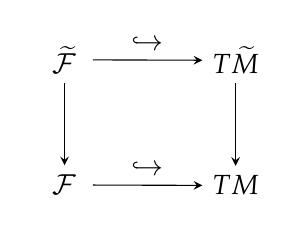
\begin{tikzpicture}
\matrix (m) [matrix of math nodes,row sep=3em,column sep=4em,minimum width=2em]
{
	\widetilde{\mathcal F} &    T\widetilde{M} \\
	\mathcal F	& TM    \\};
\path[-stealth]
(m-1-1) edge node [above] {$\hookto$} (m-1-2)
(m-1-1) edge node [right] {} (m-2-1)
(m-1-2) edge node [right] {} (m-2-2)
(m-2-1) edge node [above] {$\hookto$}  (m-2-2);

\end{tikzpicture}
\newline
then $\widetilde{\mathcal F}$ is integrable.

\begin{definition}\label{fol_cov_defn}
In the above situation we say that a foliation $\left(\widetilde{M},~ \widetilde{\mathcal F} \right)$ is the \textit{induced by} $p$ \textit{covering} of $\left(M,\mathcal F \right)$ or the $p$-\textit{lift} of $\left(M,\mathcal F \right)$. 
\end{definition}
\begin{remark}
The $p$-lift of a foliation is described in  \cite{ouchi:cov_fol, xiaolu:foli_cov}.
\end{remark}
\begin{empt}
If $\gamma: \left[0,1\right]\to M$ is a path which corresponds to an element of the holonomy groupoid then we denote by $\left[\gamma\right]$ its equivalence class, i.e. element of groupoid.
There is the space of half densities $\Omega_{\widetilde{M}}^{1/2}$ on $\widetilde{M}$ which is a lift  the space of half densities $\Omega_{M}^{1/2}$ on $M$. If $L$ is a leaf of $\left(M,\mathcal F \right)$, $L'=\pi^{-1}\left( L\right)$   then a space $\widetilde{L}$ of holonomy covering of  $L$ coincides with the space of the holonomy covering of $L'$. It turns out that $L^2\left( \widetilde{\mathcal G}_{\widetilde{x}}\right)\approx L^2\left(\mathcal G_{ \pi\left(\widetilde{x}\right)} \right)$ for any $\widetilde{x} \in \widetilde{M}$.
If $\mathcal G$ (resp. $\widetilde{\mathcal G}$) is a holonomy groupoid of $\left(M,\mathcal F \right)$ (resp. $\left(\widetilde{M},~ \widetilde{\mathcal F} \right)$) then there is the surjective map $p_{\mathcal G}:\widetilde{\mathcal G} \to \mathcal G$ given by
\begin{equation*}
	\begin{split}
		\left[\widetilde{\gamma}\right] \mapsto \left[p \circ\widetilde{\gamma}\right].
	\end{split}
\end{equation*}
If the covering is finite-fold then the map $p_{\mathcal G}:\widetilde{\mathcal G} \to \mathcal G$ induces 
a natural involutive homomorphism
\begin{equation*}
	\begin{split}
		\Coo_c\left(\mathcal G,  \Omega_{M}^{1/2}\right) \hookto  \Coo_c\left(\widetilde{\mathcal G},  \Omega_{\widetilde{M}}^{1/2}\right).
	\end{split}
\end{equation*}	
Completions of $\Coo_c\left(\mathcal G,  \Omega_{M}^{1/2}\right)$ and $\Coo_c\left(\widetilde{\mathcal G},  \Omega_{\widetilde{M}}^{1/2}\right)$ with respect to given by \eqref{foli_pseudo_norm_eqn} norms gives an injective *- homomorphism 
\be\label{foli_inc_eqn}
\pi: C^*_r\left( M,\mathcal F\right) \hookto C^*_r\left(\widetilde{M},~ \widetilde{\mathcal F} \right)
\ee
of $C^*$-algebras. The action of the group $G\left( \left.\widetilde{M}~\right|M\right)$ of covering transformations on $\widetilde{M}$ naturally induces an action of $G\left( \left.\widetilde{M}~\right|M\right)$ on $\left(\widetilde{M},~ \widetilde{\mathcal F} \right)$.  It follows that there is the natural action   $C^*_r\left(\widetilde{M},~ \widetilde{\mathcal F} \right)$ such that 
\be\label{foli_exp_g_eqn}
C^*_r\left( M, \mathcal{F}\right)   = C^*_r\left(\widetilde{M},~ \widetilde{\mathcal F} \right)^{G\left( \left.\widetilde{M}~\right|M\right)}
\ee
\end{empt}

Let $\G\left({M},~ {\mathcal F} \right)$ and $\G\left(\widetilde{M},~ \widetilde{\mathcal F} \right)$ be the holonomy groupoids of $\left({M},~ {\mathcal F} \right)$ and $\left(\widetilde{M},~ \widetilde{\mathcal F} \right)$ respectively. The natural surjective map $\G\left(\widetilde{M},~ \widetilde{\mathcal F} \right)\to\G\left({M},~ {\mathcal F} \right)$ induces the injective *-homomorphism $C_r^*\left(\widetilde{M},~ \widetilde{\mathcal F} \right)\hookto C^*_r\left(\widetilde{M},~ \widetilde{\mathcal F} \right)$.
Assume both $\G\left({M},~ {\mathcal F} \right)$ and $\G\left(\widetilde{M},~ \widetilde{\mathcal F} \right)$ are Hausdorff. Let $G\left( \left.\widetilde{M}~\right|M\right)$  be the covering 	group of  $p:\widetilde M \to M$ . The $G\left( \left.\widetilde{M}~\right|M\right)$-action on $\widetilde{M}$ can be naturally extended to $\G\left(\widetilde{M},~ \widetilde{\mathcal F} \right)$ by sending $\widetilde{\ga}$ to $g\widetilde{\ga}$ for a representative path $\widetilde{\ga}$ in $ \widetilde{M}$ and $g \in G\left( \left.\widetilde{M}~\right|M\right)$. %Therefore we have a transformation groupoid $G\left( \left.\widetilde{M}~\right|M\right)\times \G\left(\widetilde{M},~ \widetilde{\mathcal F} \right)$, with the composition law $\left(g',g\widetilde{\ga} \right)\left(g, \widetilde{\ga}\right) =  \left(g'g, \widetilde{\ga}\right)$.  	 Let $G = \G\left({M},~ {\mathcal F} \right)$, $H = G\left( \left.\widetilde{M}~\right|M\right)\times \G\left(\widetilde{M},~ \widetilde{\mathcal F} \right)$, and $Z = \G\left(\widetilde{M},~ \widetilde{\mathcal F} \right)$. Clearly, the  		unit spaces are $G^0 = M$ and $H^0 = M$. Define $\rho: Z \to G^0$ and $\sigma: Z \to H^0$ by $\rho\left(\widetilde{\ga}\right)= p\left(r\left(\widetilde{\ga} \right)  \right)$  $\sigma\left( \widetilde{\ga}\right) = p\left(r\left( \widetilde{\ga}\right)  \right)$. Both are continuous open maps. The space $Z$ is
\begin{lemma}\cite{xiaolu:foli_cov}
Let $p:\widetilde M \to M$ be a regular covering manifold with covering group $G\left( \left.\widetilde{M}~\right|M\right)$
$N\subset M$ a connected submanifold, and $\widetilde N$ a connected component of $p^{-1}\left( N\right) $
Then the restriction $p_{\widetilde N}$ of $p$ to $N$ is also regular, with the covering group $G\left( \left.\widetilde{N}~\right|N\right)$ being a  	subgroup  $G\left( \left.\widetilde{M}~\right|M\right)$.
\end{lemma}
In particular, if $L_{\widetilde x}$ is the leave in $\left(\widetilde{M},~ \widetilde{\mathcal F} \right)$ containing $\widetilde x \in p^{-1}\left( x\right)$ , where $x \in M$,
then $L_{\widetilde x}$ is a regular cover of $L_x$. We denote the covering group by $G\left( \left.\widetilde{M}~\right|M\right)_x$. On the  other hand, for each $x \in M$, there is a holonomy group $\G^x_x$, and we have the holonomy group bundle $\left\{\G^x_x\right\}$ over $M$. If $x_1$, $x_2$ are on the same leaf, then any path $\ga$  connecting $x_1$ and $x_2$ induces an isomorphism $\ga^*: \G^{x_1}_{x_1}\xrightarrow{\cong}\G^{x_2}_{x_2}$  by mapping $\left[\ga_1\right]$ to $\left[\ga\ga_1\ga^{-1}\right]$.
As a local homeomorphism, the covering map $p$ induces an embedding $\overline{p} : \G^{\widetilde x}_{\widetilde x}\to \G^x_x$ for each $\widetilde x \in p^{-1}\left( x\right)$.
\begin{lemma}\cite{xiaolu:foli_cov}
The group $\overline{p}^*_x\left(\G^{\widetilde x}_{\widetilde x}\right)$ is a normal subgroup of $G^x_x$. Equivalently,
$\overline{p}^*_x\left( \G^{\widetilde x_1}_{\widetilde x_1}\right) =\overline{p}^*_x\left( \G^{\widetilde x_2}_{\widetilde x_2}\right)$ for $\widetilde x_1, \widetilde x_2 \in p^{-1}\left(x\right)$ if $L_{\widetilde x_1}=L_{\widetilde x_2}$,
\end{lemma}
Thus we may form the quotient holonomy group bundle $\left\{\G^{\widetilde x}_{\widetilde x}\right\}$ over $M$. There is an obvious group homomorphism $\phi_x: G\left( \left.\widetilde{M}~\right|M\right)_x \to \G^{ x}_{ x}/\G^{\widetilde x}_{\widetilde x}$ defined as follows. An element $g\in G\left( \left.\widetilde{M}~\right|M\right)_x$ corresponds to a point $x_g \in p^{-1}\left( x\right)\cap L_{\widetilde x}$ if we fix $\widetilde x$ corresponding
to the unit $e$. A path $\ga_g$ starting at  $\widetilde x$ and ending at $g \widetilde x$ gives a loop $\pi\left(\widetilde \ga_g \right)$  in $M$ representing an element $\phi_x\left(g \right)$  in $G_x$, whose class in $\G^{ x}_{ x}/\G^{\widetilde x}_{\widetilde x}$ is uniquely defined
by $g$. Given any $\left[\ga\right]$ in $\G^{ x}_{ x}$ there is a preimage $\widetilde \ga$ in $L_{\widetilde x}$ starting at $\widetilde x$. The point $r\left( \widetilde \ga\right) \in p^{-1}\left( x\right)\cap  L_{\widetilde x}$ corresponding to some $g\in G\left( \left.\widetilde{M}~\right|M\right)_x$. So $\phi_x$ is onto.
\begin{definition}\cite{xiaolu:foli_cov}\label{foli_reg_cov_defn}
The covering map $p:\left(\widetilde{M},~ \widetilde{\mathcal F} \right)\to\left({M},~ {\mathcal F} \right)$ of foliations is said to be \textit{regular} if the map $\phi$ is an isomorphism from the leaf covering group bundle to the quotient holonomy group bundle.
\end{definition}

\begin{remark}\label{foli_action_rem}
Every regular covering map $p:\left(\widetilde{M},~ \widetilde{\mathcal F} \right)\to\left({M},~ {\mathcal F} \right)$ of foliations induces nontrivial action of $G\left( \left.\widetilde{M}~\right|M\right)$ on $C^*_r\left(\widetilde{M},~ \widetilde{\mathcal F}  \right)$ such that $$C^*_r\left(\widetilde{M},~ \widetilde{\mathcal F}  \right)^{ G\left( \left.\widetilde{M}~\right|M\right)}\cong C^*_r\left(\widetilde{M},~ \widetilde{\mathcal F}  \right).$$
\end{remark}
\begin{remark}\label{foli_trans_rem}
If a map $p:\left(\widetilde{M},~ \widetilde{\mathcal F} \right)\to\left({M},~ {\mathcal F} \right)$ is regular covering of foliations  and a leaf $\widetilde L \in \widetilde M$ has no holonomy then  $g\widetilde L \neq \widetilde L$ for all nontrivial $g \in G\left( \left.\widetilde{M}~\right|M\right)$, i.e. $G\left( \left.\widetilde{M}~\right|M\right)$ transitively acts on leaves having no holonomy.
\end{remark}

	\end{appendices}
			
%\section*{Acknowledgment}


%\paragraph*{}
% I am grateful to my grandfather Petr who forested my mind and my grandson Petr who  watched my work.
 

 
 \begin{thebibliography}{10}
 	


%\bibitem{godement:sheaf} Roger Godement, \textit{Topologie Alg�brique et Th�orie des Faisceaux}. Actualit�s Sci. Ind. No. 1252. Publ. Math. Univ. Strasbourg. No. 13 Hermann, Paris. 1958.

%\bibitem{goldblatt:topoi} Robert Goldblatt. \textit{Topoi: The Categorial Analysis of Logic}. Revised edition of XLVII 445. Studies in logic and the foundations of mathematics, vol. 98. North-Holland, Amsterdam, New York, and Oxford, 1984, xvi + 551 pp. 1984.
\bibitem{bryl:loop}Jean-Luc Brylinski. \textit{Loop Spaces, Characteristic Classes and Geometric Quantization}. Springer Science \& Business Media, Nov 15, 2007.

\bibitem{cuntz_meyer_ros:bivariant} Joachim Cuntz, Ralf Meyer, Jonathan M. Rosenberg.
\textit{Topological and Bivariant K-Theory}. (Oberwolfach Seminars, 36, Band 36) 2010.
\bibitem{eust} Samuel Eilenberg, Norman E. Steenrod \textit{Foundations of Algebraic Topology}. Published by Princeton University Press 1952.
%\bibitem{dimca:sheaves} Alexandru Dimca. \textit{Sheaves in Topology} Springer Science \& Business Media, Mar 12, 2004. 

\bibitem{engelking:general_topology} Ryszard Engelking. \textit{General topology}, PWN, Warsaw. 1977.

%\bibitem{gelfand_manin} Sergei I. Gelfand, Yuri I. Manin. \textit{Methods of Homological Algebra},  Springer Monographs in Mathematics (SMM), 1996.

\bibitem{hartshorne:ag} Robin Hartshorne. {\it Algebraic Geometry.} Graduate Texts in Mathematics, Volume 52, 1977.

\bibitem{matro:hcm} Manuilov V.M., Troitsky E.V. \textit{Hilbert $C^*$-modules}. % Publication Year: 2005. ISBN-10: 0-8218-3810-5 ISBN-13: 978-0-8218-3810-5 
Translations of Mathematical Monographs, vol. 226, 2005.

\bibitem{milne:lec} J.S. Milne. \textit{Lectures on \'Etale Cohomology}. Version 2.21 March 22, 2013.

\bibitem{murphy}G.J. Murphy. {\it $C^*$-Algebras and Operator Theory.} Academic Press 1990.



\bibitem{johnstone:topos}P.T. Johnstone. \textit{Topos Theory}, L. M. S. Monographs no. 10, Academic Press 1977.

\bibitem{pedersen:ca_aut}Gert Kj�rg�rd Pedersen. {\it $C^*$-algebras and their automorphism groups}. London ; New York : Academic Press, 1979.

\bibitem{rae:ctr_morita} Iain Raeburn, Dana P. Williams. \textit{Morita Equivalence and Continuous-trace $C^*$-algebras}. American Mathematical Soc., 1998.





\end{thebibliography}




 \end{document}


